\documentclass[oneside]{book}
\usepackage[bookmarks=true, colorlinks, linkcolor=gray]{hyperref}
\usepackage[top=1in, bottom=1in, left=1.25in, right=1.25in]{geometry}
\usepackage{cite}
\usepackage{graphicx}
\usepackage{float}
\usepackage{listings}
\usepackage{color}

% Packages required by doxygen
\usepackage{fixltx2e}
\usepackage{calc}
\usepackage{doxygen}
\usepackage[export]{adjustbox} % also loads graphicx
\usepackage{graphicx}
\usepackage[utf8]{inputenc}
\usepackage{makeidx}
\usepackage{multicol}
\usepackage{multirow}
\PassOptionsToPackage{warn}{textcomp}
\usepackage{textcomp}
\usepackage[nointegrals]{wasysym}
\usepackage[table]{xcolor}


% \renewcommand\thesection{\arabic{section}}

\definecolor{mygreen}{rgb}{0,0.6,0}
\definecolor{mygray}{rgb}{0.5,0.5,0.5}
\definecolor{mymauve}{rgb}{0.58,0,0.82}

\lstset{ %
  backgroundcolor=\color{white},   % choose the background color; you must add \usepackage{color} or \usepackage{xcolor}
  basicstyle=\footnotesize\ttfamily,        % the size of the fonts that are used for the code
  breakatwhitespace=false,         % sets if automatic breaks should only happen at whitespace
  breaklines=true,                 % sets automatic line breaking
  captionpos=b,                    % sets the caption-position to bottom
  commentstyle=\color{mygreen}\ttfamily,    % comment style
  frame=single,	                   % adds a frame around the code
  keepspaces=true,                 % keeps spaces in text, useful for keeping indentation of code (possibly needs columns=flexible)
  keywordstyle=\color{blue},       % keyword style
  language=C++,                    % the language of the code
  rulecolor=\color{black},         % if not set, the frame-color may be changed on line-breaks within not-black text (e.g. comments (green here))
  showspaces=false,                % show spaces everywhere adding particular underscores; it overrides 'showstringspaces'
  showstringspaces=false,          % underline spaces within strings only
  showtabs=false,                  % show tabs within strings adding particular underscores
  stepnumber=2,                    % the step between two line-numbers. If it's 1, each line will be numbered
  stringstyle=\color{mymauve},     % string literal style
  tabsize=2,	                   % sets default tabsize to 2 spaces
}

\usepackage{caption}
\captionsetup{labelsep=space,justification=centering,font={bf},singlelinecheck=off,skip=4pt,position=top}

% Add search path
\makeatletter
\providecommand*\input@path{}
\newcommand*\addinputpath[1]{%
  \expandafter\def\expandafter\input@path
  \expandafter{\input@path#1}}%
\addinputpath{{doxygen/}}
\makeatother

\graphicspath{{doxygen/}{UML/}{interface/}}

% �½ڲ���ҳ
\usepackage{xpatch}
\makeatletter
\xpatchcmd{\chapter}
  {\if@openright\cleardoublepage\else\clearpage\fi}{\par\relax}
  {}{}
\makeatother

\makeatletter
\xpatchcmd{\part}
  {\if@openright\cleardoublepage\else\clearpage\fi}{\par\relax}
  {}{}
\makeatother

\title{\textbf{Individual Project 2\\ Constructing Minimum Spanning Trees\\ Software Design Document}}
\author{Zhang Huimeng, 2015011280}

\begin{document}

\maketitle
\author
\clearpage

\tableofcontents
\clearpage


\part{Introduction}

    \chapter{Purpose}

        This software design document describes the architecture and system design of project ComputeMST. This is a homework of Fundamentals of Object-Oriented Programming class, Spring 2016. The homework requirement is as follows:

         (II) Project: On Constructing Minimum Spanning Trees (Difficulty: 1.1)

        Requirements and TIPS:

        (1) Implement the MST algorithm based on Voronoi diagram for computing Euclidean minimum spanning trees in 2D plane.

        (2) Please refer to \href{http://www.cs.princeton.edu/courses/archive/spr07/cos226/lectures/mst.pdf}{the following link} for MST construction algorithms. Either Prim's or Kruskal's algorithm is ok. Please refer to Page 39 for the idea of using Voronoi for MST computation.

        (3) Use the \href{http://www.cgal.org/}{CGAL Library} for constructing the Voronoi diagram and Delaunay triangulation.

        (4) Randomly generate 5 different testcases with more than 5000 points without duplicates to test the implemented method.

        (5) It is suggested that a validity checking function be implemented to verify the experimental results are correct. For example, you may directly apply Prim's or Kruskal's MST algorithm on the testcase to verify that the MST trees are correct.

        (6) Report the statistics of the experimental results, e.g., total runtime, total number of points, total length of the MST edges, etc. Figures and tables on the experimental results are welcome.

        (7) [This is not mandatory to finish, but it is a challenging topic] Again, can you compute the top K ($1 <= K <= 20$) minimum spanning trees?

    \chapter{Scope}

        I implemented the first six requirements of the homework, mainly using CGAL and Kruskal's MST algorithm. The program can load input from file or randomly generate input for itself; it has a GUI interface and can print results of the MST computation to file.

\clearpage
\part{System Overview}

    The program can compute Delaunay triangulation (via CGAL library) and MST for up to 10000 points in a 2-dimensional plane in 1 or 2 seconds. It can output the result to file. Also, it has a interface written with Freeglut.

\clearpage
\part{System Architecture}

    \chapter{Architectural Design} % ������ϵͳ����Ϊ����ģ�飬����ÿ��ģ��֮��Ĺ��ܺ��໥��ϵ

        The program can be divided into three parts: the Basics part, the Computational part and the Display part.

        \begin{center}
        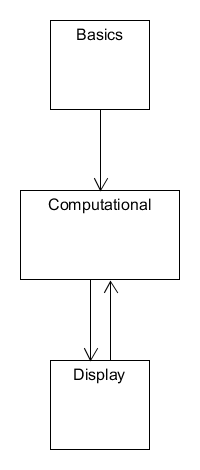
\includegraphics[width=\linewidth / 3]{main.png}
        \end{center}

        The basics part provides some useful tools for the Computational part, like statistics and timer.

        The computational part does the computation, and interacts with the Display part to provide a workable interface.

        The display part deals with the interface and user input.

    \chapter{Decomposition Description}

        \section{Basics}

            The \hyperlink{classcmst_1_1_stat}{Stat} class deals with statistics. It receives data in the form of floating-point number and can work continuously. It calculates the mean, maximum, minimum and standard deviation of the data.

            \begin{center}
            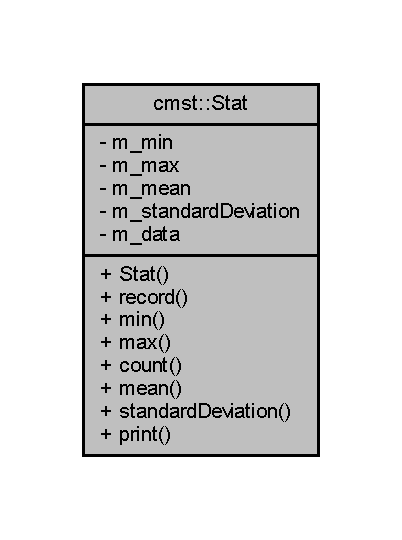
\includegraphics[width=\linewidth / 3]{classcmst_1_1_stat__coll__graph}
            \end{center}

            The \hyperlink{classcmst_1_1_timer}{Timer} class deals with timing. It uses the clock() function.

            \begin{center}
            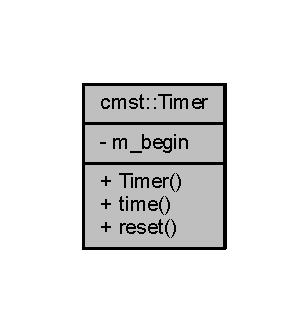
\includegraphics[width=\linewidth / 3]{classcmst_1_1_timer__coll__graph}
            \end{center}

        \section{Computational}

            The \hyperlink{classcmst_1_1_point2_d}{Point2D}, \hyperlink{classcmst_1_1_edge2_d}{Edge2D} and \hyperlink{classcmst_1_1_index_edge2_d}{IndexEdge2D} classes are the basic 2-dimensional computational geometry classes.

            \begin{center}
            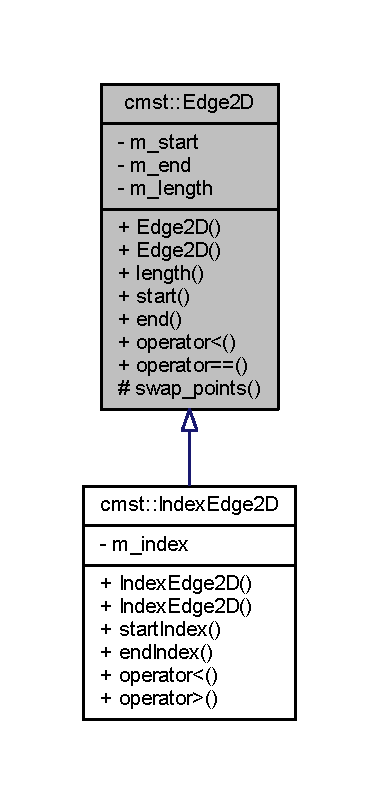
\includegraphics[width=\linewidth / 3]{classcmst_1_1_edge2_d__inherit__graph}
            \end{center}

            \begin{center}
            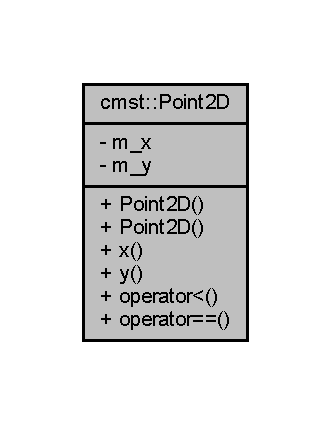
\includegraphics[width=\linewidth / 3]{classcmst_1_1_point2_d__coll__graph}
            \end{center}

            The \hyperlink{classcmst_1_1_graph2_d}{Graph2D} class deals with all the computations. The Delaunay triangulation and MST are computed in the constructor. This class also provides drawing functions that draw the graph by Freeglut.

            \begin{center}
            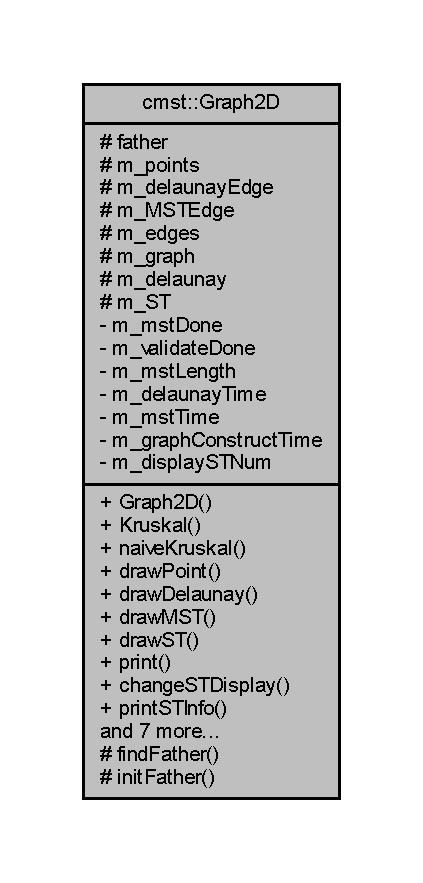
\includegraphics[width=\linewidth / 3]{classcmst_1_1_graph2_d__coll__graph}
            \end{center}

            It also contains a nested struct, \hyperlink{structcmst_1_1_graph2_d_1_1_s_t}{Graph2D::ST} that stores spanning trees of the graph. If I had time, I would have implemented the k-top spanning tree calculation.

        \section{Display}

            The Display part contains the Freeglut window and pop-up menu management functions, as well as the \hyperlink{classcmst_1_1_window}{Window} class that manages the window. Here is the UML diagram of this class:

            \begin{center}
            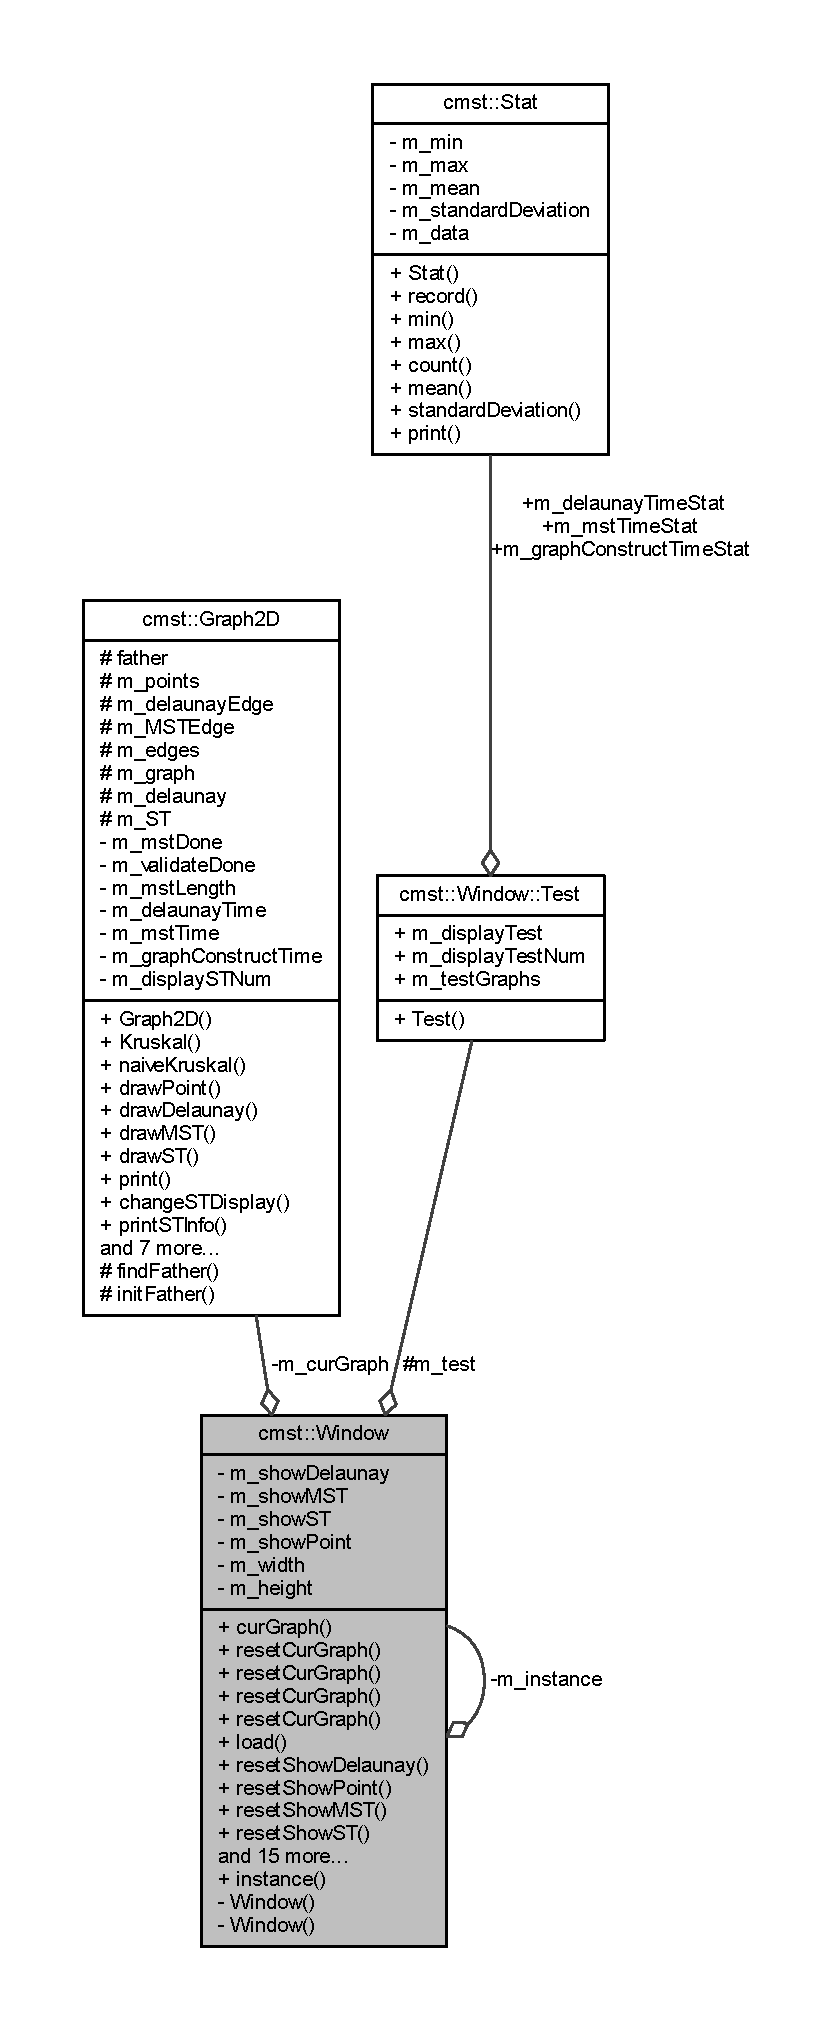
\includegraphics[width=\linewidth / 2]{classcmst_1_1_window__coll__graph}
            \end{center}


\clearpage
\part{Data Design}

    \chapter{Data Description} % data structure, data storage, process and organization

        The program uses very simple ways of managing data: most data is stored in vectors and arrays.

\clearpage
\part{Human Interface Design}

    \chapter{Overview of Human Interface}

        Here is a screen shot of the main screen:

        \begin{center}
        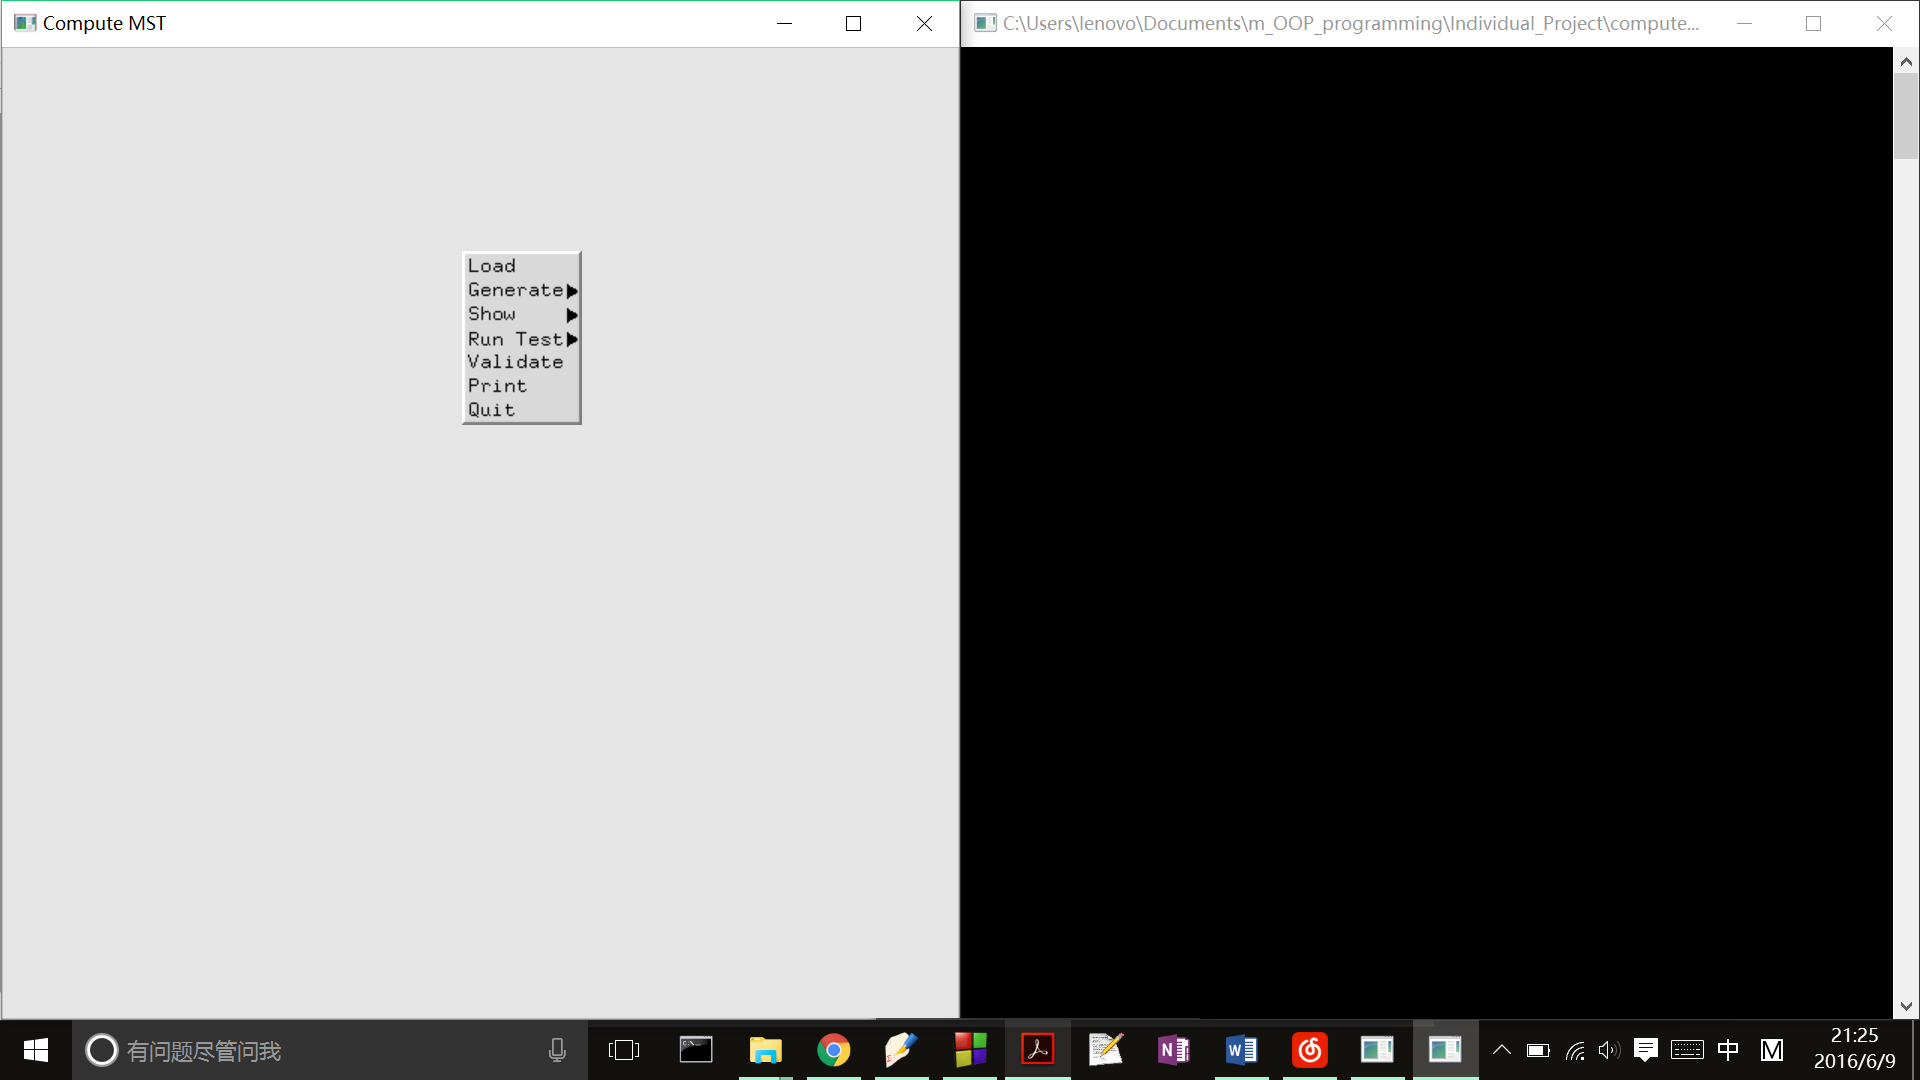
\includegraphics[width=\linewidth]{main_interface.png}
        \end{center}

        On the left is the Freeglut window, and the console is on the right. If you right-click on the glut window, a pop-up window will appear, as in the screenshot above. The console prints information about graphs and MSTs being displayed in the window.

        \section{Main Menu}

            \begin{center}
            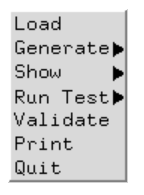
\includegraphics[width=\linewidth / 3]{main_menu.png}
            \end{center}

            As can be seen from the screenshot above, main menu has 7 menu entries:
            \begin{description}
              \item[Load] This option loads point information from a file to construct the graph. There are some requirements of the input. You have to provide the full path to the input file.
              \item[Generate] See \ref{'Generate' sub-Menu}.
              \item[Show] See \ref{'Show' sub-Menu}.
              \item[Run Test] See \ref{'Run Test' sub-Menu}.
              \item[Validate] Run the validating naive MST algorithm for the graph.
              \item[Print] Print information to graph.txt.
              \item[Quit] Exit the program.
            \end{description}

        \section{'Generate' sub-Menu}
        \label{'Generate' sub-Menu}

            \begin{center}
            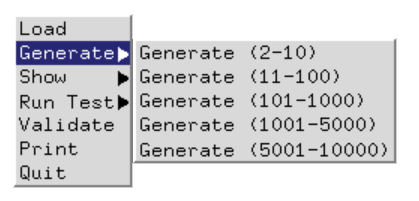
\includegraphics[width=\linewidth / 3]{generate_menu.png}
            \end{center}

            This sub-menu has 5 menu entries:
            \begin{description}
              \item[Generate(2-10)] Generate 2-10 points.
              \item[Generate(11-100)] Generate 11-100 points.
              \item[Generate(101-1000)] Generate 101-1000 points.
              \item[Generate(1001-5000)] Generate 1001-5000 points.
              \item[Generate(5001-10000)] Generate 5001-10000 points.
            \end{description}

        \section{'Show' sub-Menu}
        \label{'Show' sub-Menu}

            \begin{center}
            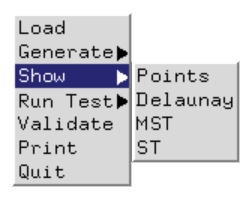
\includegraphics[width=\linewidth / 3]{show_menu.png}
            \end{center}

            This sub-menu has 4 menu entries:
            \begin{description}
              \item[Points] Whether the points are drawn.
              \item[Delaunay] Whether the Delaunay triangulation is drawn.
              \item[MST] Whether the MST is draw.
              \item[ST] Whether the STs are drawn. These include the MST calculated in validating and other spanning trees.
            \end{description}

        \section{'Run Test' sub-Menu}
        \label{'Run Test' sub-Menu}

            \begin{center}
            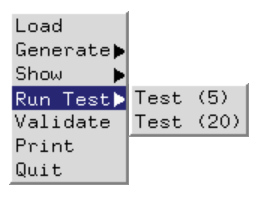
\includegraphics[width=\linewidth / 3]{test_menu.png}
            \end{center}

            This sub-menu has 2 menu entries:
            \begin{description}
              \item[Test(5)] Run a test of 5 graphs, each having 10000 points.
              \item[Test(20)] Run a test of 20 graphs, each having 10000 points.
            \end{description}

            After a test is run, you can use left and right arrow keys to move through test graphs.

    \chapter{Screen Images}

        \begin{figure}[H]
          \centering
          % Requires \usepackage{graphicx}
          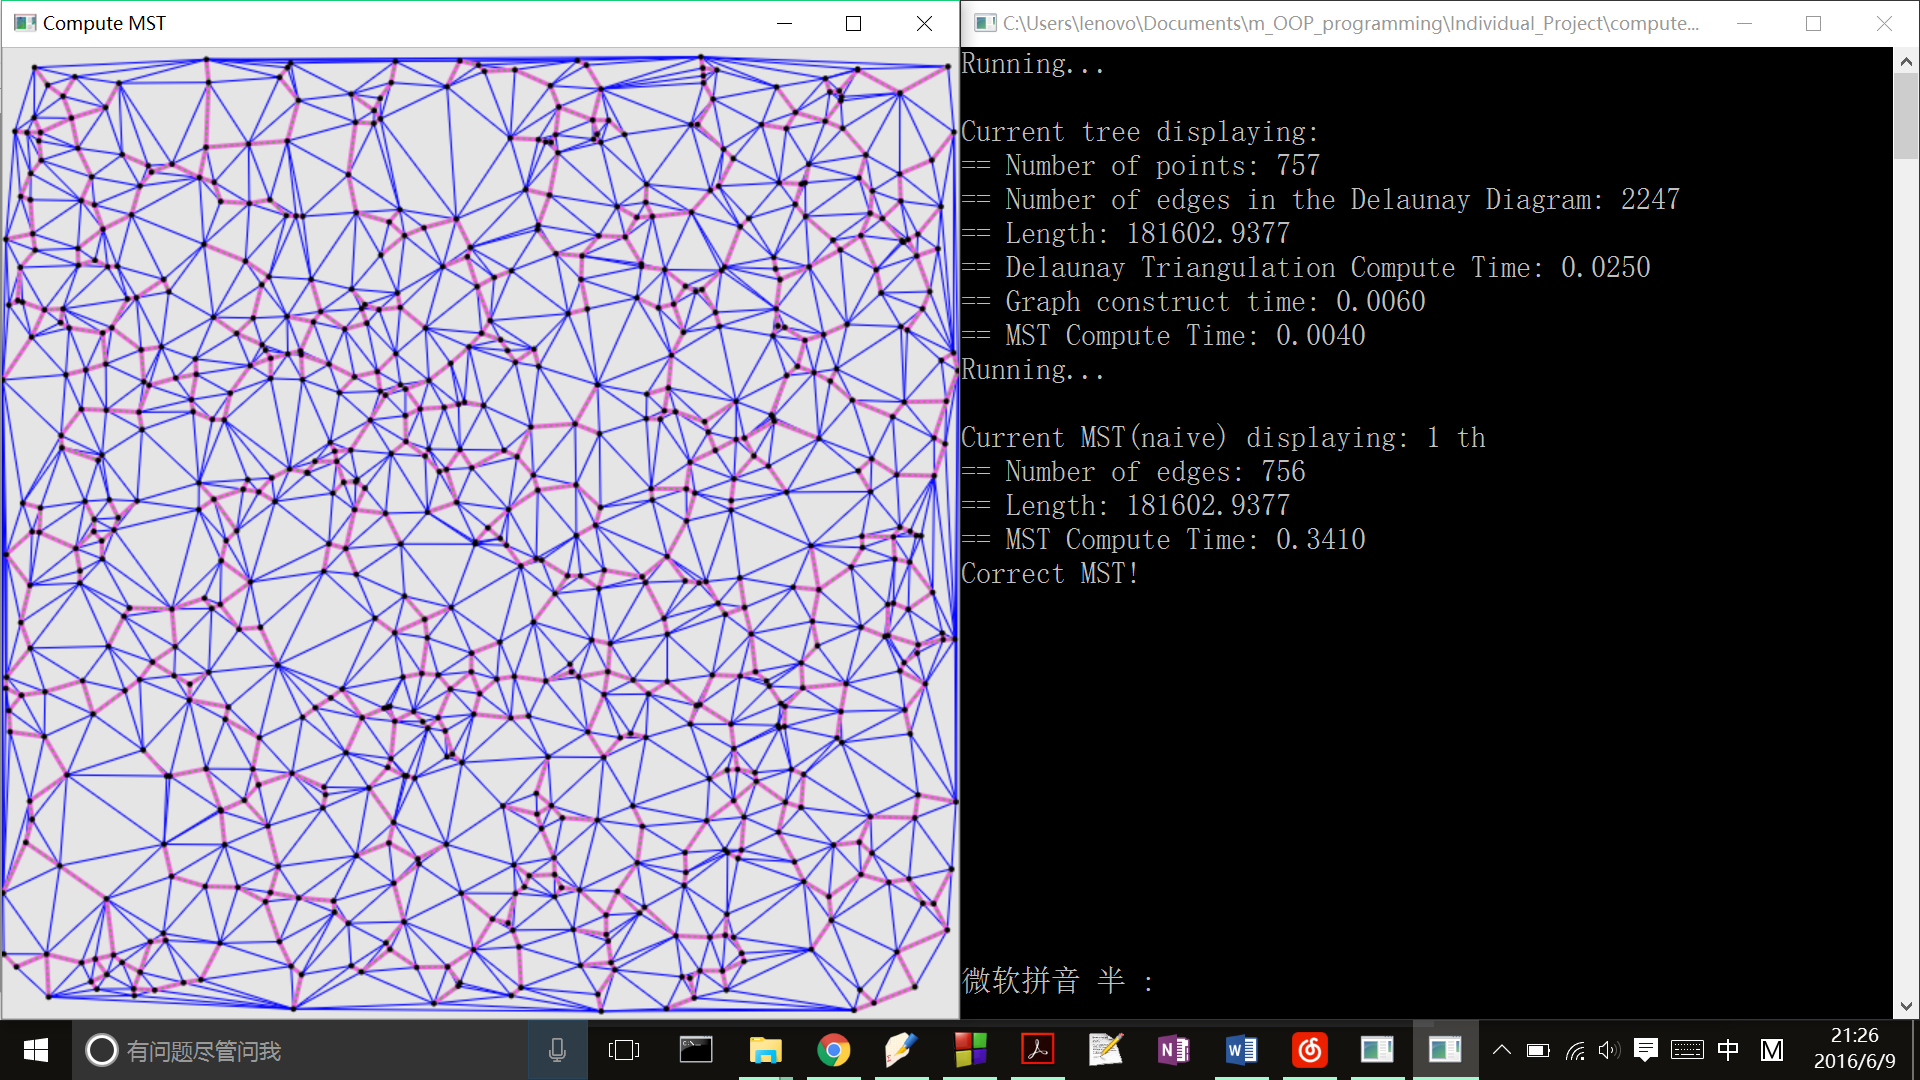
\includegraphics[width=\linewidth]{after_generating}\\
          \caption{After a graph is generated}\label{after_generating}
        \end{figure}

        Delaunay triangulation is drawn in thin blue lines, and MST is drawn in thick pink lines. Spanning trees are drawn in dotted lines.

        \begin{figure}[H]
          \centering
          % Requires \usepackage{graphicx}
          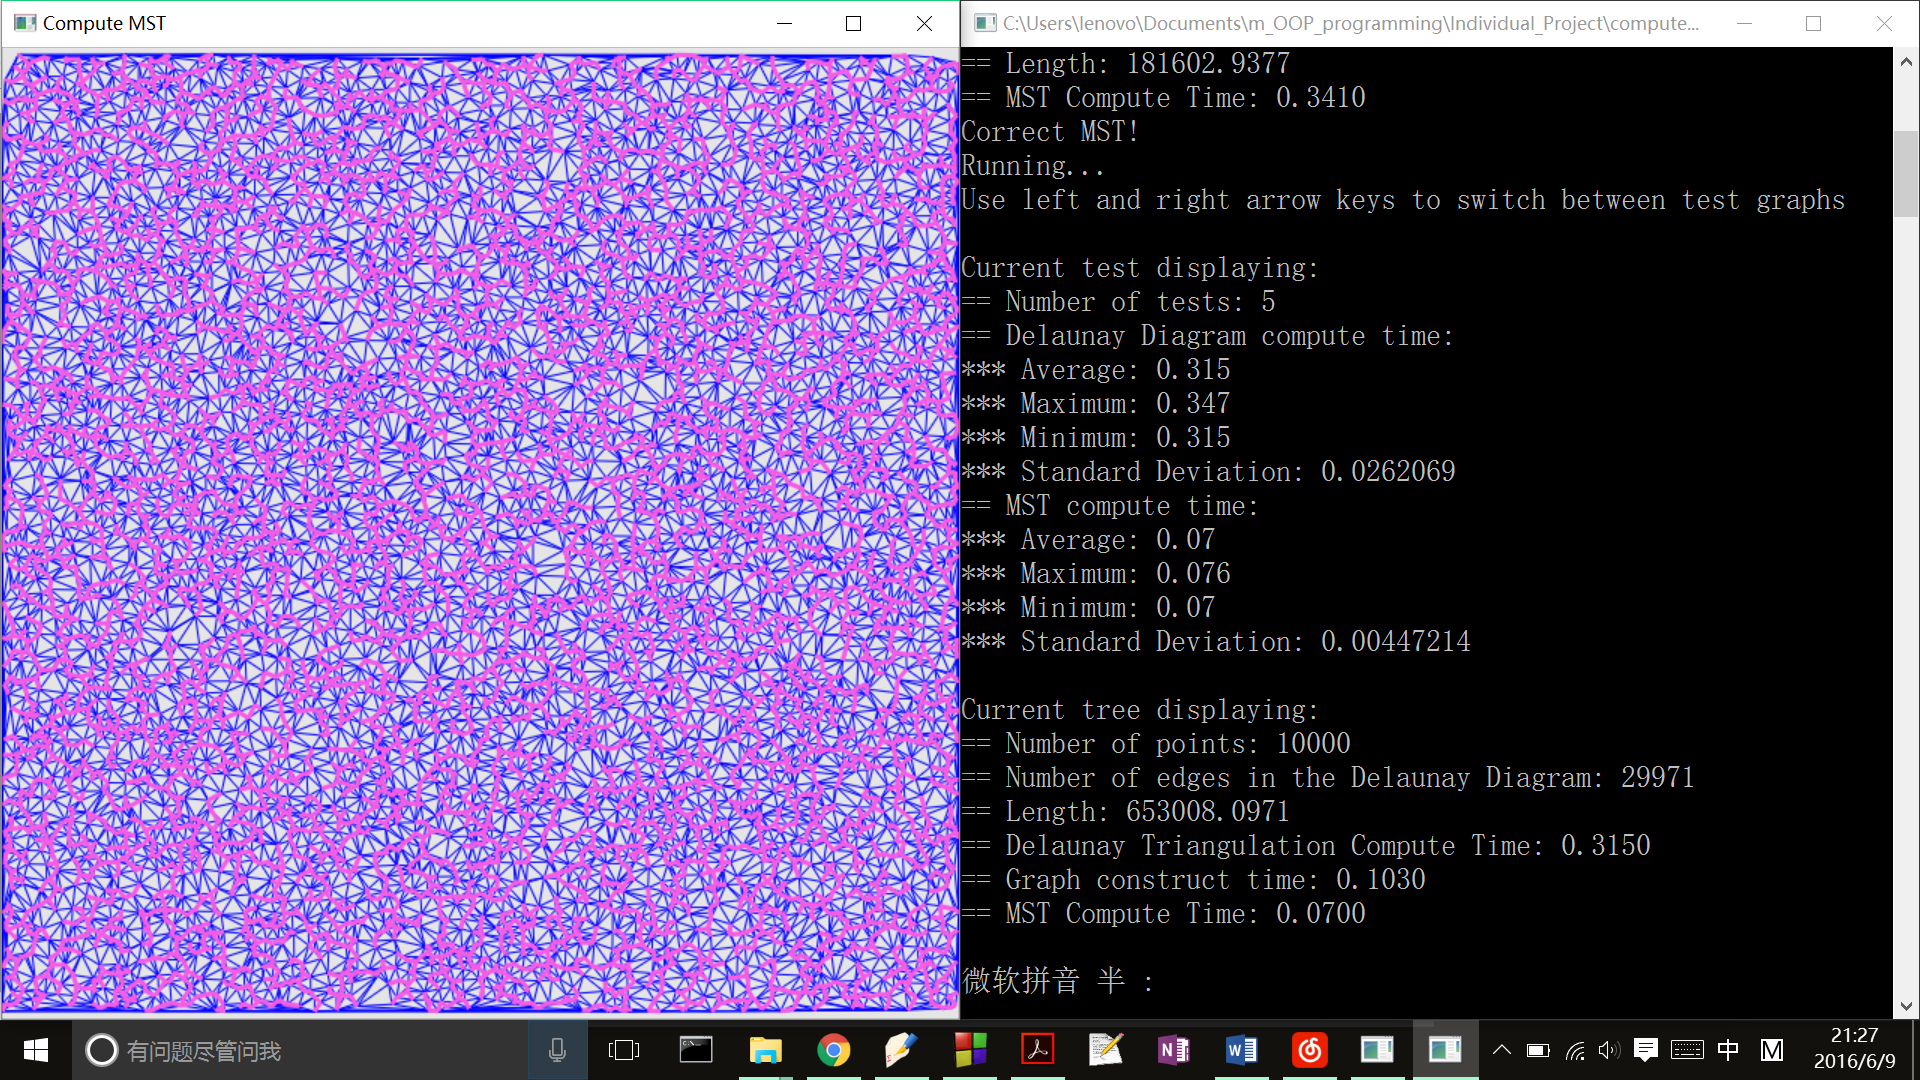
\includegraphics[width=\linewidth]{after_test}\\
          \caption{After running a test}\label{after_test}
        \end{figure}

        In the above screenshot, the points and spanning trees are not drawn.

        \begin{figure}[H]
          \centering
          % Requires \usepackage{graphicx}
          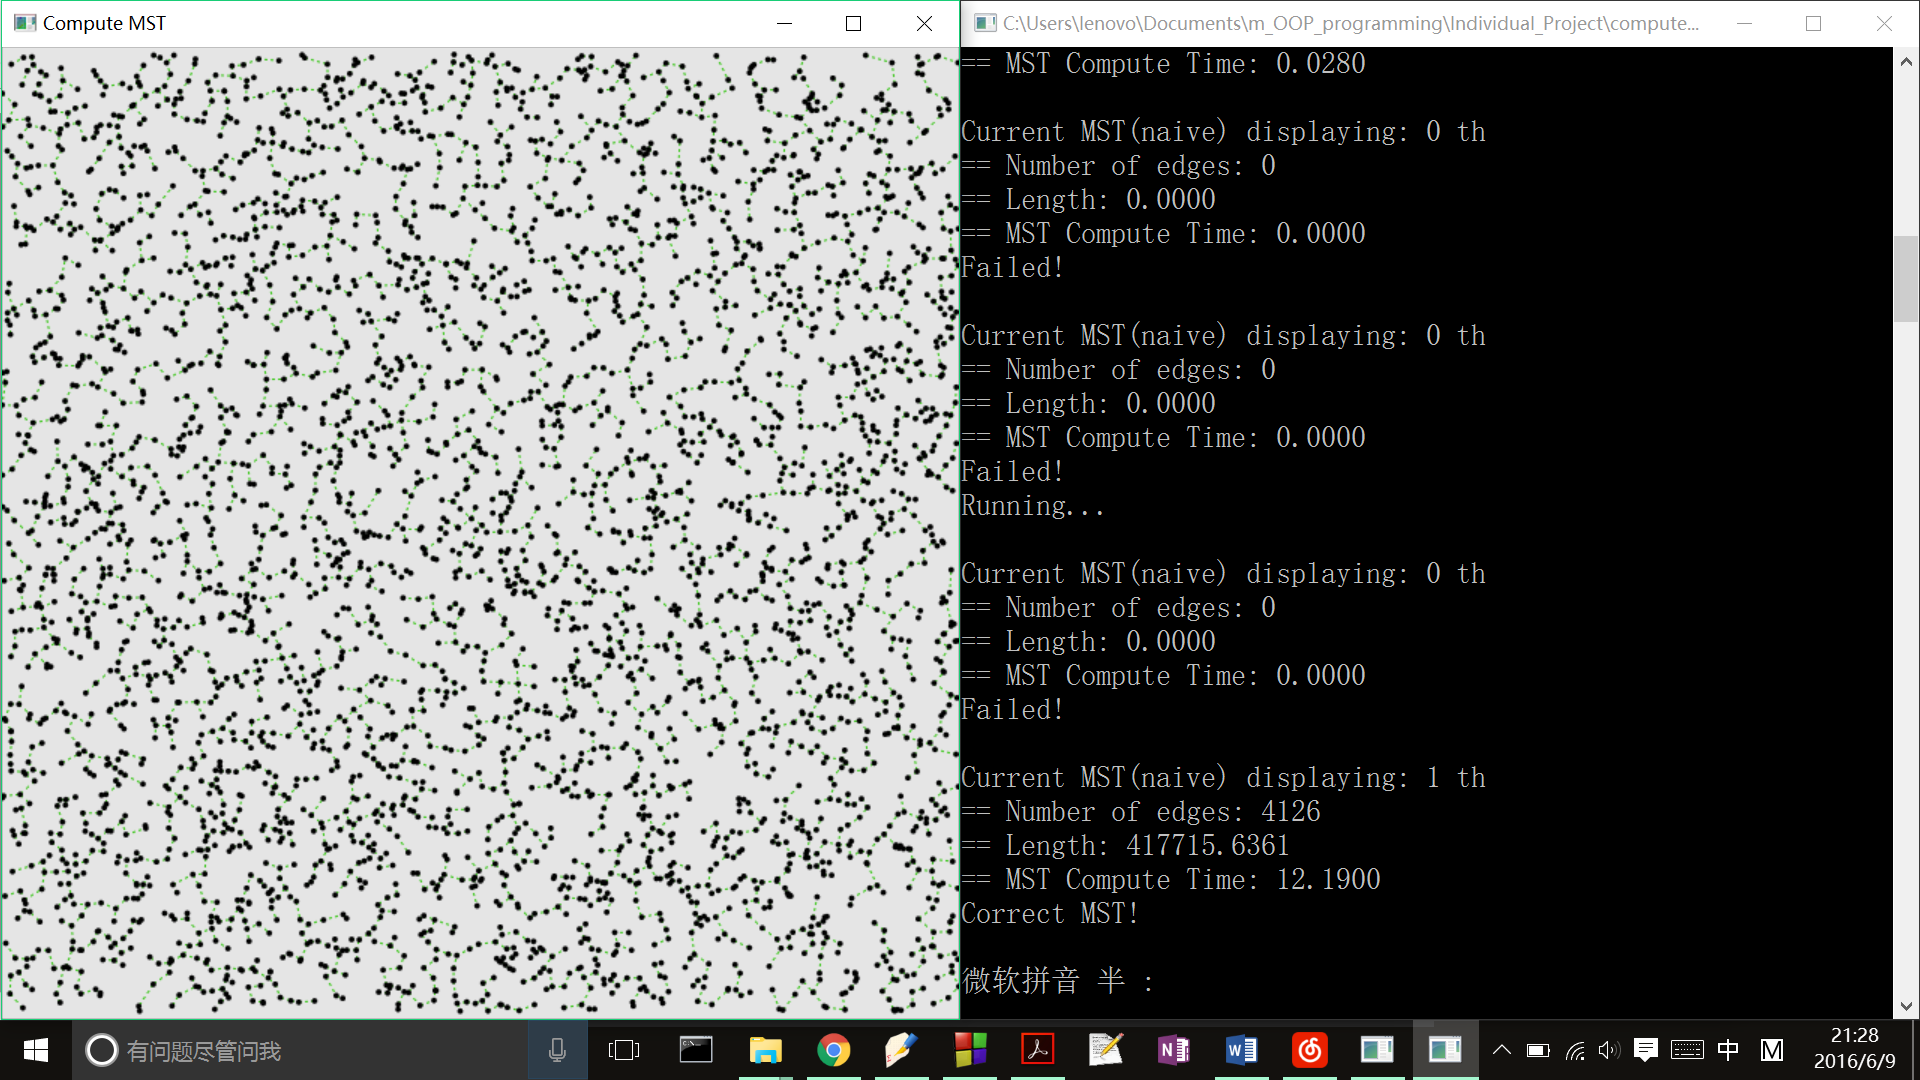
\includegraphics[width=\linewidth]{after_validate}\\
          \caption{After running a validate}\label{after_validate}
        \end{figure}

        In the above screenshot, the Delaunay triangulation and MST are not drawn.

\clearpage
\part{Design Patterns}

    \chapter{Singleton}

        This program uses Singleton pattern in \hyperlink{classcmst_1_1_window}{Window}. There can only be one main window in one program.

\clearpage
\part{Component Design}
%--- Begin generated contents ---
\chapter{Namespace Index}
\section{Namespace List}
Here is a list of all namespaces with brief descriptions:\begin{DoxyCompactList}
\item\contentsline{section}{\hyperlink{namespacecmst}{cmst} }{\pageref{namespacecmst}}{}
\end{DoxyCompactList}

\chapter{Hierarchical Index}
\section{Class Hierarchy}
This inheritance list is sorted roughly, but not completely, alphabetically:\begin{DoxyCompactList}
\item \contentsline{section}{cmst::Edge2D}{\pageref{classcmst_1_1_edge2_d}}{}
\begin{DoxyCompactList}
\item \contentsline{section}{cmst::IndexEdge2D}{\pageref{classcmst_1_1_index_edge2_d}}{}
\end{DoxyCompactList}
\item \contentsline{section}{cmst::Graph2D}{\pageref{classcmst_1_1_graph2_d}}{}
\item \contentsline{section}{cmst::Point2D}{\pageref{classcmst_1_1_point2_d}}{}
\item \contentsline{section}{cmst::Graph2D::ST}{\pageref{structcmst_1_1_graph2_d_1_1_s_t}}{}
\item \contentsline{section}{cmst::Stat}{\pageref{classcmst_1_1_stat}}{}
\item \contentsline{section}{cmst::Window::Test}{\pageref{structcmst_1_1_window_1_1_test}}{}
\item \contentsline{section}{cmst::Timer}{\pageref{classcmst_1_1_timer}}{}
\item \contentsline{section}{cmst::Window}{\pageref{classcmst_1_1_window}}{}
\end{DoxyCompactList}

\chapter{Class Index}
\section{Class List}
Here are the classes, structs, unions and interfaces with brief descriptions:\begin{DoxyCompactList}
\item\contentsline{section}{\hyperlink{classcmst_1_1_edge2_d}{cmst::Edge2D} }{\pageref{classcmst_1_1_edge2_d}}{}
\item\contentsline{section}{\hyperlink{classcmst_1_1_graph2_d}{cmst::Graph2D} }{\pageref{classcmst_1_1_graph2_d}}{}
\item\contentsline{section}{\hyperlink{classcmst_1_1_index_edge2_d}{cmst::IndexEdge2D} \\*Edge with start and end point indices in an array }{\pageref{classcmst_1_1_index_edge2_d}}{}
\item\contentsline{section}{\hyperlink{classcmst_1_1_point2_d}{cmst::Point2D} \\*Points in a 2D plane }{\pageref{classcmst_1_1_point2_d}}{}
\item\contentsline{section}{\hyperlink{structcmst_1_1_graph2_d_1_1_s_t}{cmst::Graph2D::ST} \\*Store a spanning tree of the graph }{\pageref{structcmst_1_1_graph2_d_1_1_s_t}}{}
\item\contentsline{section}{\hyperlink{classcmst_1_1_stat}{cmst::Stat} }{\pageref{classcmst_1_1_stat}}{}
\item\contentsline{section}{\hyperlink{structcmst_1_1_window_1_1_test}{cmst::Window::Test} }{\pageref{structcmst_1_1_window_1_1_test}}{}
\item\contentsline{section}{\hyperlink{classcmst_1_1_timer}{cmst::Timer} }{\pageref{classcmst_1_1_timer}}{}
\item\contentsline{section}{\hyperlink{classcmst_1_1_window}{cmst::Window} }{\pageref{classcmst_1_1_window}}{}
\end{DoxyCompactList}

\chapter{Namespace Documentation}
\hypertarget{namespacecmst}{}\section{cmst Namespace Reference}
\label{namespacecmst}\index{cmst@{cmst}}
\subsection*{Classes}
\begin{DoxyCompactItemize}
\item 
class \hyperlink{classcmst_1_1_edge2_d}{Edge2D}
\item 
class \hyperlink{classcmst_1_1_graph2_d}{Graph2D}
\item 
class \hyperlink{classcmst_1_1_index_edge2_d}{Index\+Edge2D}
\begin{DoxyCompactList}\small\item\em Edge with start and end point indices in an array. \end{DoxyCompactList}\item 
class \hyperlink{classcmst_1_1_point2_d}{Point2D}
\begin{DoxyCompactList}\small\item\em Points in a 2D plane. \end{DoxyCompactList}\item 
class \hyperlink{classcmst_1_1_stat}{Stat}
\item 
class \hyperlink{classcmst_1_1_timer}{Timer}
\item 
class \hyperlink{classcmst_1_1_window}{Window}
\end{DoxyCompactItemize}
\subsection*{Enumerations}
\begin{DoxyCompactItemize}
\item 
enum \hyperlink{namespacecmst_a8dff7ccfde8a2770160b5f8dbf81c3b9}{Menu} \{ \\*
\hyperlink{namespacecmst_a8dff7ccfde8a2770160b5f8dbf81c3b9a2664ea87b6a9f05151f0706429b5a65f}{L\+O\+AD}, 
\hyperlink{namespacecmst_a8dff7ccfde8a2770160b5f8dbf81c3b9acc1b341b1550c4009942f0a14b433fb5}{N\+EW}, 
\hyperlink{namespacecmst_a8dff7ccfde8a2770160b5f8dbf81c3b9a5c1bbae108fea09abee0ae385bc729bf}{N\+E\+W\+\_\+4\+\_\+10}, 
\hyperlink{namespacecmst_a8dff7ccfde8a2770160b5f8dbf81c3b9a613b1d9e468c6e26e23c33a2abb2833e}{N\+E\+W\+\_\+11\+\_\+100}, 
\\*
\hyperlink{namespacecmst_a8dff7ccfde8a2770160b5f8dbf81c3b9a7ca958e9941ebe27acf2ae7511b735ba}{N\+E\+W\+\_\+101\+\_\+1000}, 
\hyperlink{namespacecmst_a8dff7ccfde8a2770160b5f8dbf81c3b9a35fe2b5c1c0015c3aee5049bee8b8acd}{N\+E\+W\+\_\+1001\+\_\+5000}, 
\hyperlink{namespacecmst_a8dff7ccfde8a2770160b5f8dbf81c3b9a73f732474a8fd1746e18e85ac18965f0}{N\+E\+W\+\_\+5001\+\_\+10000}, 
\hyperlink{namespacecmst_a8dff7ccfde8a2770160b5f8dbf81c3b9a4484f6b658f88772d77bfeaaa19b7a11}{S\+H\+OW}, 
\\*
\hyperlink{namespacecmst_a8dff7ccfde8a2770160b5f8dbf81c3b9acb33c06abf6f54d270a6a6f26b3b0ec4}{S\+H\+O\+W\+\_\+\+V\+O\+R\+O\+N\+OI}, 
\hyperlink{namespacecmst_a8dff7ccfde8a2770160b5f8dbf81c3b9a4a94d06c45900d709f4714d9fdebb3f0}{S\+H\+O\+W\+\_\+\+D\+E\+L\+A\+U\+N\+AY}, 
\hyperlink{namespacecmst_a8dff7ccfde8a2770160b5f8dbf81c3b9ac4fb0b335b5fbcbc4f68b7adff95928d}{S\+H\+O\+W\+\_\+\+P\+O\+I\+NT}, 
\hyperlink{namespacecmst_a8dff7ccfde8a2770160b5f8dbf81c3b9a800b0742385b3bd700ac88151b5b15de}{S\+H\+O\+W\+\_\+\+M\+ST}, 
\\*
\hyperlink{namespacecmst_a8dff7ccfde8a2770160b5f8dbf81c3b9ae0df18e68aebe2f40f7e6f8ca8454203}{S\+H\+O\+W\+\_\+\+ST}, 
\hyperlink{namespacecmst_a8dff7ccfde8a2770160b5f8dbf81c3b9a95c752e50b27aaae9aa758293828007f}{T\+E\+ST}, 
\hyperlink{namespacecmst_a8dff7ccfde8a2770160b5f8dbf81c3b9a9996ad31ad035f42371059ad53098246}{T\+E\+S\+T\+\_\+5}, 
\hyperlink{namespacecmst_a8dff7ccfde8a2770160b5f8dbf81c3b9a3f5dd18e08446227f6ce81fed096c339}{T\+E\+S\+T\+\_\+20}, 
\\*
\hyperlink{namespacecmst_a8dff7ccfde8a2770160b5f8dbf81c3b9a8718984584621ce08ac6c64133ce08d2}{V\+A\+L\+I\+D\+A\+T\+OR}, 
\hyperlink{namespacecmst_a8dff7ccfde8a2770160b5f8dbf81c3b9abb9d71d90223f47e4008e0ac05b93938}{P\+R\+I\+NT}, 
\hyperlink{namespacecmst_a8dff7ccfde8a2770160b5f8dbf81c3b9af46a16cac81f794824d0d87fb5588e33}{Q\+U\+IT}
 \}\begin{DoxyCompactList}\small\item\em Return values for G\+L\+UT menus. \end{DoxyCompactList}
\end{DoxyCompactItemize}
\subsection*{Functions}
\begin{DoxyCompactItemize}
\item 
int \hyperlink{namespacecmst_a844037f018f3d5b7b1f1a5f4463da501}{random\+Int} (int a, int b)
\item 
double \hyperlink{namespacecmst_a8df08a5847caeb65a6606968e40f336f}{random\+Double} (double a, double b)
\item 
std\+::vector$<$ \hyperlink{classcmst_1_1_point2_d}{Point2D} $>$ \hyperlink{namespacecmst_abd1822f67dc5d2be959508e628be0633}{Testcase\+Generator} (int num\+\_\+lower\+\_\+bound=100, int num\+\_\+upper\+\_\+bound=500, double x\+\_\+upper\+\_\+bound=M\+A\+X\+\_\+X, double y\+\_\+upper\+\_\+bound=M\+A\+X\+\_\+Y)
\end{DoxyCompactItemize}


\subsection{Enumeration Type Documentation}
\index{cmst@{cmst}!Menu@{Menu}}
\index{Menu@{Menu}!cmst@{cmst}}
\subsubsection[{\texorpdfstring{Menu}{Menu}}]{\setlength{\rightskip}{0pt plus 5cm}enum {\bf cmst\+::\+Menu}}\hypertarget{namespacecmst_a8dff7ccfde8a2770160b5f8dbf81c3b9}{}\label{namespacecmst_a8dff7ccfde8a2770160b5f8dbf81c3b9}


Return values for G\+L\+UT menus. 

\begin{Desc}
\item[Enumerator]\par
\begin{description}
\index{L\+O\+AD@{L\+O\+AD}!cmst@{cmst}}\index{cmst@{cmst}!L\+O\+AD@{L\+O\+AD}}\item[{\em 
L\+O\+AD\hypertarget{namespacecmst_a8dff7ccfde8a2770160b5f8dbf81c3b9a2664ea87b6a9f05151f0706429b5a65f}{}\label{namespacecmst_a8dff7ccfde8a2770160b5f8dbf81c3b9a2664ea87b6a9f05151f0706429b5a65f}
}]\index{N\+EW@{N\+EW}!cmst@{cmst}}\index{cmst@{cmst}!N\+EW@{N\+EW}}\item[{\em 
N\+EW\hypertarget{namespacecmst_a8dff7ccfde8a2770160b5f8dbf81c3b9acc1b341b1550c4009942f0a14b433fb5}{}\label{namespacecmst_a8dff7ccfde8a2770160b5f8dbf81c3b9acc1b341b1550c4009942f0a14b433fb5}
}]\index{N\+E\+W\+\_\+4\+\_\+10@{N\+E\+W\+\_\+4\+\_\+10}!cmst@{cmst}}\index{cmst@{cmst}!N\+E\+W\+\_\+4\+\_\+10@{N\+E\+W\+\_\+4\+\_\+10}}\item[{\em 
N\+E\+W\+\_\+4\+\_\+10\hypertarget{namespacecmst_a8dff7ccfde8a2770160b5f8dbf81c3b9a5c1bbae108fea09abee0ae385bc729bf}{}\label{namespacecmst_a8dff7ccfde8a2770160b5f8dbf81c3b9a5c1bbae108fea09abee0ae385bc729bf}
}]\index{N\+E\+W\+\_\+11\+\_\+100@{N\+E\+W\+\_\+11\+\_\+100}!cmst@{cmst}}\index{cmst@{cmst}!N\+E\+W\+\_\+11\+\_\+100@{N\+E\+W\+\_\+11\+\_\+100}}\item[{\em 
N\+E\+W\+\_\+11\+\_\+100\hypertarget{namespacecmst_a8dff7ccfde8a2770160b5f8dbf81c3b9a613b1d9e468c6e26e23c33a2abb2833e}{}\label{namespacecmst_a8dff7ccfde8a2770160b5f8dbf81c3b9a613b1d9e468c6e26e23c33a2abb2833e}
}]\index{N\+E\+W\+\_\+101\+\_\+1000@{N\+E\+W\+\_\+101\+\_\+1000}!cmst@{cmst}}\index{cmst@{cmst}!N\+E\+W\+\_\+101\+\_\+1000@{N\+E\+W\+\_\+101\+\_\+1000}}\item[{\em 
N\+E\+W\+\_\+101\+\_\+1000\hypertarget{namespacecmst_a8dff7ccfde8a2770160b5f8dbf81c3b9a7ca958e9941ebe27acf2ae7511b735ba}{}\label{namespacecmst_a8dff7ccfde8a2770160b5f8dbf81c3b9a7ca958e9941ebe27acf2ae7511b735ba}
}]\index{N\+E\+W\+\_\+1001\+\_\+5000@{N\+E\+W\+\_\+1001\+\_\+5000}!cmst@{cmst}}\index{cmst@{cmst}!N\+E\+W\+\_\+1001\+\_\+5000@{N\+E\+W\+\_\+1001\+\_\+5000}}\item[{\em 
N\+E\+W\+\_\+1001\+\_\+5000\hypertarget{namespacecmst_a8dff7ccfde8a2770160b5f8dbf81c3b9a35fe2b5c1c0015c3aee5049bee8b8acd}{}\label{namespacecmst_a8dff7ccfde8a2770160b5f8dbf81c3b9a35fe2b5c1c0015c3aee5049bee8b8acd}
}]\index{N\+E\+W\+\_\+5001\+\_\+10000@{N\+E\+W\+\_\+5001\+\_\+10000}!cmst@{cmst}}\index{cmst@{cmst}!N\+E\+W\+\_\+5001\+\_\+10000@{N\+E\+W\+\_\+5001\+\_\+10000}}\item[{\em 
N\+E\+W\+\_\+5001\+\_\+10000\hypertarget{namespacecmst_a8dff7ccfde8a2770160b5f8dbf81c3b9a73f732474a8fd1746e18e85ac18965f0}{}\label{namespacecmst_a8dff7ccfde8a2770160b5f8dbf81c3b9a73f732474a8fd1746e18e85ac18965f0}
}]\index{S\+H\+OW@{S\+H\+OW}!cmst@{cmst}}\index{cmst@{cmst}!S\+H\+OW@{S\+H\+OW}}\item[{\em 
S\+H\+OW\hypertarget{namespacecmst_a8dff7ccfde8a2770160b5f8dbf81c3b9a4484f6b658f88772d77bfeaaa19b7a11}{}\label{namespacecmst_a8dff7ccfde8a2770160b5f8dbf81c3b9a4484f6b658f88772d77bfeaaa19b7a11}
}]\index{S\+H\+O\+W\+\_\+\+V\+O\+R\+O\+N\+OI@{S\+H\+O\+W\+\_\+\+V\+O\+R\+O\+N\+OI}!cmst@{cmst}}\index{cmst@{cmst}!S\+H\+O\+W\+\_\+\+V\+O\+R\+O\+N\+OI@{S\+H\+O\+W\+\_\+\+V\+O\+R\+O\+N\+OI}}\item[{\em 
S\+H\+O\+W\+\_\+\+V\+O\+R\+O\+N\+OI\hypertarget{namespacecmst_a8dff7ccfde8a2770160b5f8dbf81c3b9acb33c06abf6f54d270a6a6f26b3b0ec4}{}\label{namespacecmst_a8dff7ccfde8a2770160b5f8dbf81c3b9acb33c06abf6f54d270a6a6f26b3b0ec4}
}]\index{S\+H\+O\+W\+\_\+\+D\+E\+L\+A\+U\+N\+AY@{S\+H\+O\+W\+\_\+\+D\+E\+L\+A\+U\+N\+AY}!cmst@{cmst}}\index{cmst@{cmst}!S\+H\+O\+W\+\_\+\+D\+E\+L\+A\+U\+N\+AY@{S\+H\+O\+W\+\_\+\+D\+E\+L\+A\+U\+N\+AY}}\item[{\em 
S\+H\+O\+W\+\_\+\+D\+E\+L\+A\+U\+N\+AY\hypertarget{namespacecmst_a8dff7ccfde8a2770160b5f8dbf81c3b9a4a94d06c45900d709f4714d9fdebb3f0}{}\label{namespacecmst_a8dff7ccfde8a2770160b5f8dbf81c3b9a4a94d06c45900d709f4714d9fdebb3f0}
}]\index{S\+H\+O\+W\+\_\+\+P\+O\+I\+NT@{S\+H\+O\+W\+\_\+\+P\+O\+I\+NT}!cmst@{cmst}}\index{cmst@{cmst}!S\+H\+O\+W\+\_\+\+P\+O\+I\+NT@{S\+H\+O\+W\+\_\+\+P\+O\+I\+NT}}\item[{\em 
S\+H\+O\+W\+\_\+\+P\+O\+I\+NT\hypertarget{namespacecmst_a8dff7ccfde8a2770160b5f8dbf81c3b9ac4fb0b335b5fbcbc4f68b7adff95928d}{}\label{namespacecmst_a8dff7ccfde8a2770160b5f8dbf81c3b9ac4fb0b335b5fbcbc4f68b7adff95928d}
}]\index{S\+H\+O\+W\+\_\+\+M\+ST@{S\+H\+O\+W\+\_\+\+M\+ST}!cmst@{cmst}}\index{cmst@{cmst}!S\+H\+O\+W\+\_\+\+M\+ST@{S\+H\+O\+W\+\_\+\+M\+ST}}\item[{\em 
S\+H\+O\+W\+\_\+\+M\+ST\hypertarget{namespacecmst_a8dff7ccfde8a2770160b5f8dbf81c3b9a800b0742385b3bd700ac88151b5b15de}{}\label{namespacecmst_a8dff7ccfde8a2770160b5f8dbf81c3b9a800b0742385b3bd700ac88151b5b15de}
}]\index{S\+H\+O\+W\+\_\+\+ST@{S\+H\+O\+W\+\_\+\+ST}!cmst@{cmst}}\index{cmst@{cmst}!S\+H\+O\+W\+\_\+\+ST@{S\+H\+O\+W\+\_\+\+ST}}\item[{\em 
S\+H\+O\+W\+\_\+\+ST\hypertarget{namespacecmst_a8dff7ccfde8a2770160b5f8dbf81c3b9ae0df18e68aebe2f40f7e6f8ca8454203}{}\label{namespacecmst_a8dff7ccfde8a2770160b5f8dbf81c3b9ae0df18e68aebe2f40f7e6f8ca8454203}
}]\index{T\+E\+ST@{T\+E\+ST}!cmst@{cmst}}\index{cmst@{cmst}!T\+E\+ST@{T\+E\+ST}}\item[{\em 
T\+E\+ST\hypertarget{namespacecmst_a8dff7ccfde8a2770160b5f8dbf81c3b9a95c752e50b27aaae9aa758293828007f}{}\label{namespacecmst_a8dff7ccfde8a2770160b5f8dbf81c3b9a95c752e50b27aaae9aa758293828007f}
}]\index{T\+E\+S\+T\+\_\+5@{T\+E\+S\+T\+\_\+5}!cmst@{cmst}}\index{cmst@{cmst}!T\+E\+S\+T\+\_\+5@{T\+E\+S\+T\+\_\+5}}\item[{\em 
T\+E\+S\+T\+\_\+5\hypertarget{namespacecmst_a8dff7ccfde8a2770160b5f8dbf81c3b9a9996ad31ad035f42371059ad53098246}{}\label{namespacecmst_a8dff7ccfde8a2770160b5f8dbf81c3b9a9996ad31ad035f42371059ad53098246}
}]\index{T\+E\+S\+T\+\_\+20@{T\+E\+S\+T\+\_\+20}!cmst@{cmst}}\index{cmst@{cmst}!T\+E\+S\+T\+\_\+20@{T\+E\+S\+T\+\_\+20}}\item[{\em 
T\+E\+S\+T\+\_\+20\hypertarget{namespacecmst_a8dff7ccfde8a2770160b5f8dbf81c3b9a3f5dd18e08446227f6ce81fed096c339}{}\label{namespacecmst_a8dff7ccfde8a2770160b5f8dbf81c3b9a3f5dd18e08446227f6ce81fed096c339}
}]\index{V\+A\+L\+I\+D\+A\+T\+OR@{V\+A\+L\+I\+D\+A\+T\+OR}!cmst@{cmst}}\index{cmst@{cmst}!V\+A\+L\+I\+D\+A\+T\+OR@{V\+A\+L\+I\+D\+A\+T\+OR}}\item[{\em 
V\+A\+L\+I\+D\+A\+T\+OR\hypertarget{namespacecmst_a8dff7ccfde8a2770160b5f8dbf81c3b9a8718984584621ce08ac6c64133ce08d2}{}\label{namespacecmst_a8dff7ccfde8a2770160b5f8dbf81c3b9a8718984584621ce08ac6c64133ce08d2}
}]\index{P\+R\+I\+NT@{P\+R\+I\+NT}!cmst@{cmst}}\index{cmst@{cmst}!P\+R\+I\+NT@{P\+R\+I\+NT}}\item[{\em 
P\+R\+I\+NT\hypertarget{namespacecmst_a8dff7ccfde8a2770160b5f8dbf81c3b9abb9d71d90223f47e4008e0ac05b93938}{}\label{namespacecmst_a8dff7ccfde8a2770160b5f8dbf81c3b9abb9d71d90223f47e4008e0ac05b93938}
}]\index{Q\+U\+IT@{Q\+U\+IT}!cmst@{cmst}}\index{cmst@{cmst}!Q\+U\+IT@{Q\+U\+IT}}\item[{\em 
Q\+U\+IT\hypertarget{namespacecmst_a8dff7ccfde8a2770160b5f8dbf81c3b9af46a16cac81f794824d0d87fb5588e33}{}\label{namespacecmst_a8dff7ccfde8a2770160b5f8dbf81c3b9af46a16cac81f794824d0d87fb5588e33}
}]\end{description}
\end{Desc}


\subsection{Function Documentation}
\index{cmst@{cmst}!random\+Double@{random\+Double}}
\index{random\+Double@{random\+Double}!cmst@{cmst}}
\subsubsection[{\texorpdfstring{random\+Double(double a, double b)}{randomDouble(double a, double b)}}]{\setlength{\rightskip}{0pt plus 5cm}double cmst\+::random\+Double (
\begin{DoxyParamCaption}
\item[{double}]{a, }
\item[{double}]{b}
\end{DoxyParamCaption}
)}\hypertarget{namespacecmst_a8df08a5847caeb65a6606968e40f336f}{}\label{namespacecmst_a8df08a5847caeb65a6606968e40f336f}
Generate a floating-\/point number in the range \mbox{[}a, b\mbox{]}

Needs to be improved using other random classes 

Here is the caller graph for this function\+:
% FIG 0


\index{cmst@{cmst}!random\+Int@{random\+Int}}
\index{random\+Int@{random\+Int}!cmst@{cmst}}
\subsubsection[{\texorpdfstring{random\+Int(int a, int b)}{randomInt(int a, int b)}}]{\setlength{\rightskip}{0pt plus 5cm}int cmst\+::random\+Int (
\begin{DoxyParamCaption}
\item[{int}]{a, }
\item[{int}]{b}
\end{DoxyParamCaption}
)}\hypertarget{namespacecmst_a844037f018f3d5b7b1f1a5f4463da501}{}\label{namespacecmst_a844037f018f3d5b7b1f1a5f4463da501}
Generate an integer in the range \mbox{[}a, b\mbox{]}

Needs to be improved using other random classes 

Here is the caller graph for this function\+:
% FIG 1


\index{cmst@{cmst}!Testcase\+Generator@{Testcase\+Generator}}
\index{Testcase\+Generator@{Testcase\+Generator}!cmst@{cmst}}
\subsubsection[{\texorpdfstring{Testcase\+Generator(int num\+\_\+lower\+\_\+bound=100, int num\+\_\+upper\+\_\+bound=500, double x\+\_\+upper\+\_\+bound=\+M\+A\+X\+\_\+\+X, double y\+\_\+upper\+\_\+bound=\+M\+A\+X\+\_\+\+Y)}{TestcaseGenerator(int num_lower_bound=100, int num_upper_bound=500, double x_upper_bound=MAX_X, double y_upper_bound=MAX_Y)}}]{\setlength{\rightskip}{0pt plus 5cm}std\+::vector$<$ {\bf cmst\+::\+Point2D} $>$ cmst\+::\+Testcase\+Generator (
\begin{DoxyParamCaption}
\item[{int}]{num\+\_\+lower\+\_\+bound = {\ttfamily 100}, }
\item[{int}]{num\+\_\+upper\+\_\+bound = {\ttfamily 500}, }
\item[{double}]{x\+\_\+upper\+\_\+bound = {\ttfamily MAX\+\_\+X}, }
\item[{double}]{y\+\_\+upper\+\_\+bound = {\ttfamily MAX\+\_\+Y}}
\end{DoxyParamCaption}
)}\hypertarget{namespacecmst_abd1822f67dc5d2be959508e628be0633}{}\label{namespacecmst_abd1822f67dc5d2be959508e628be0633}
Generate some random points.

The number of points is generated randomly in the range \mbox{[}num\+\_\+lower\+\_\+bound, num\+\_\+upper\+\_\+bound\mbox{]}, and the x, y coordinates of the points are respectively in the range \mbox{[}0, x\+\_\+upper\+\_\+bound\mbox{]} and \mbox{[}0, y\+\_\+upper\+\_\+bound\mbox{]}. 

Here is the call graph for this function\+:
% FIG 2




Here is the caller graph for this function\+:
% FIG 3



\chapter{Class Documentation}
\hypertarget{classcmst_1_1_edge2_d}{}\section{cmst::Edge2D Class Reference}
\label{classcmst_1_1_edge2_d}\index{cmst::Edge2D@{cmst::Edge2D}}


Inheritance diagram for cmst::Edge2D:
% FIG 0


Collaboration diagram for cmst::Edge2D:
% FIG 1
\subsection*{Public Member Functions}
\begin{DoxyCompactItemize}
\item 
\hyperlink{classcmst_1_1_edge2_d_a5af466b468749d363692f16de84a85d5}{Edge2D} ()
\item 
\hyperlink{classcmst_1_1_edge2_d_a0d1166315f84757395e889d3225e2ae0}{Edge2D} (const \hyperlink{classcmst_1_1_point2_d}{Point2D} \&\hyperlink{classcmst_1_1_edge2_d_ad77218c63818fe92f43033ba1487ab89}{start}, const \hyperlink{classcmst_1_1_point2_d}{Point2D} \&\hyperlink{classcmst_1_1_edge2_d_af02d43d8344759ac3709d318e26cdcee}{end})
\item 
double \hyperlink{classcmst_1_1_edge2_d_adaa859c8f6b412e1174abe8d8b429ce9}{length} () const 
\item 
\hyperlink{classcmst_1_1_point2_d}{Point2D} \hyperlink{classcmst_1_1_edge2_d_ad77218c63818fe92f43033ba1487ab89}{start} () const 
\item 
\hyperlink{classcmst_1_1_point2_d}{Point2D} \hyperlink{classcmst_1_1_edge2_d_af02d43d8344759ac3709d318e26cdcee}{end} () const 
\item 
bool \hyperlink{classcmst_1_1_edge2_d_ab710dba1b2f0a4c74d01a7b2c1211efa}{operator$<$} (const \hyperlink{classcmst_1_1_edge2_d}{Edge2D} \&right) const 
\begin{DoxyCompactList}\small\item\em Compares edges by length. \end{DoxyCompactList}\item 
bool \hyperlink{classcmst_1_1_edge2_d_a4370b0ab916b4fd8d5ff98733ae57116}{operator==} (const \hyperlink{classcmst_1_1_edge2_d}{Edge2D} \&right) const 
\end{DoxyCompactItemize}
\subsection*{Protected Member Functions}
\begin{DoxyCompactItemize}
\item 
void \hyperlink{classcmst_1_1_edge2_d_aeb88dc66750f6c7967de0918e906abf4}{swap\_points} ()
\begin{DoxyCompactList}\small\item\em Swaps the start and end point. \end{DoxyCompactList}\end{DoxyCompactItemize}
\subsection*{Private Attributes}
\begin{DoxyCompactItemize}
\item 
\hyperlink{classcmst_1_1_point2_d}{Point2D} \hyperlink{classcmst_1_1_edge2_d_a8c0ca77824a84a48c714aaec5da72ad7}{m\_start}
\begin{DoxyCompactList}\small\item\em Start point. \end{DoxyCompactList}\item 
\hyperlink{classcmst_1_1_point2_d}{Point2D} \hyperlink{classcmst_1_1_edge2_d_a26aabda4fcc506ae340392e78f92e49b}{m\_end}
\begin{DoxyCompactList}\small\item\em End point. \end{DoxyCompactList}\item 
double \hyperlink{classcmst_1_1_edge2_d_ab461fb636aa7f76af613c63c681c186e}{m\_length}
\begin{DoxyCompactList}\small\item\em Length. \end{DoxyCompactList}\end{DoxyCompactItemize}
\subsection*{Friends}
\begin{DoxyCompactItemize}
\item 
std::ostream \& \hyperlink{classcmst_1_1_edge2_d_ae312c205375d240b1c8bc889f2c1c55e}{operator$<$$<$} (std::ostream \&out, const \hyperlink{classcmst_1_1_edge2_d}{Edge2D} \&e)
\end{DoxyCompactItemize}


\subsection{Detailed Description}
Stores edges in 2D plane.

The start and end points are stored in the edge. 

\subsection{Constructor \& Destructor Documentation}
\index{cmst::Edge2D@{cmst::Edge2D}!Edge2D@{Edge2D}}
\index{Edge2D@{Edge2D}!cmst::Edge2D@{cmst::Edge2D}}
\subsubsection[{\texorpdfstring{Edge2D()}{Edge2D()}}]{\setlength{\rightskip}{0pt plus 5cm}cmst::Edge2D::Edge2D (
\begin{DoxyParamCaption}
{}
\end{DoxyParamCaption}
)\hspace{0.3cm}{\ttfamily [inline]}}\hypertarget{classcmst_1_1_edge2_d_a5af466b468749d363692f16de84a85d5}{}\label{classcmst_1_1_edge2_d_a5af466b468749d363692f16de84a85d5}
\index{cmst::Edge2D@{cmst::Edge2D}!Edge2D@{Edge2D}}
\index{Edge2D@{Edge2D}!cmst::Edge2D@{cmst::Edge2D}}
\subsubsection[{\texorpdfstring{Edge2D(const Point2D \&start, const Point2D \&end)}{Edge2D(const Point2D &start, const Point2D &end)}}]{\setlength{\rightskip}{0pt plus 5cm}cmst::Edge2D::Edge2D (
\begin{DoxyParamCaption}
\item[{const {\bf Point2D} \&}]{start, }
\item[{const {\bf Point2D} \&}]{end}
\end{DoxyParamCaption}
)\hspace{0.3cm}{\ttfamily [inline]}}\hypertarget{classcmst_1_1_edge2_d_a0d1166315f84757395e889d3225e2ae0}{}\label{classcmst_1_1_edge2_d_a0d1166315f84757395e889d3225e2ae0}
Constructor

Calculates the length. 

Here is the call graph for this function:
% FIG 2




\subsection{Member Function Documentation}
\index{cmst::Edge2D@{cmst::Edge2D}!end@{end}}
\index{end@{end}!cmst::Edge2D@{cmst::Edge2D}}
\subsubsection[{\texorpdfstring{end() const }{end() const }}]{\setlength{\rightskip}{0pt plus 5cm}{\bf Point2D} cmst::Edge2D::end (
\begin{DoxyParamCaption}
{}
\end{DoxyParamCaption}
) const\hspace{0.3cm}{\ttfamily [inline]}}\hypertarget{classcmst_1_1_edge2_d_af02d43d8344759ac3709d318e26cdcee}{}\label{classcmst_1_1_edge2_d_af02d43d8344759ac3709d318e26cdcee}
Returns the end point.

\begin{DoxyReturn}{Returns}
end point 
\end{DoxyReturn}


Here is the caller graph for this function:
% FIG 3


\index{cmst::Edge2D@{cmst::Edge2D}!length@{length}}
\index{length@{length}!cmst::Edge2D@{cmst::Edge2D}}
\subsubsection[{\texorpdfstring{length() const }{length() const }}]{\setlength{\rightskip}{0pt plus 5cm}double cmst::Edge2D::length (
\begin{DoxyParamCaption}
{}
\end{DoxyParamCaption}
) const\hspace{0.3cm}{\ttfamily [inline]}}\hypertarget{classcmst_1_1_edge2_d_adaa859c8f6b412e1174abe8d8b429ce9}{}\label{classcmst_1_1_edge2_d_adaa859c8f6b412e1174abe8d8b429ce9}
Returns the length of the edge.

\begin{DoxyReturn}{Returns}
length of the edge 
\end{DoxyReturn}


Here is the caller graph for this function:
% FIG 4


\index{cmst::Edge2D@{cmst::Edge2D}!operator$<$@{operator$<$}}
\index{operator$<$@{operator$<$}!cmst::Edge2D@{cmst::Edge2D}}
\subsubsection[{\texorpdfstring{operator$<$(const Edge2D \&right) const }{operator<(const Edge2D &right) const }}]{\setlength{\rightskip}{0pt plus 5cm}bool cmst::Edge2D::operator$<$ (
\begin{DoxyParamCaption}
\item[{const {\bf Edge2D} \&}]{right}
\end{DoxyParamCaption}
) const\hspace{0.3cm}{\ttfamily [inline]}}\hypertarget{classcmst_1_1_edge2_d_ab710dba1b2f0a4c74d01a7b2c1211efa}{}\label{classcmst_1_1_edge2_d_ab710dba1b2f0a4c74d01a7b2c1211efa}


Compares edges by length. 

\index{cmst::Edge2D@{cmst::Edge2D}!operator==@{operator==}}
\index{operator==@{operator==}!cmst::Edge2D@{cmst::Edge2D}}
\subsubsection[{\texorpdfstring{operator==(const Edge2D \&right) const }{operator==(const Edge2D &right) const }}]{\setlength{\rightskip}{0pt plus 5cm}bool cmst::Edge2D::operator== (
\begin{DoxyParamCaption}
\item[{const {\bf Edge2D} \&}]{right}
\end{DoxyParamCaption}
) const\hspace{0.3cm}{\ttfamily [inline]}}\hypertarget{classcmst_1_1_edge2_d_a4370b0ab916b4fd8d5ff98733ae57116}{}\label{classcmst_1_1_edge2_d_a4370b0ab916b4fd8d5ff98733ae57116}
Compares \hyperlink{classcmst_1_1_edge2_d}{cmst::Edge2D} by start point and end point.

Take the \hyperlink{classcmst_1_1_edge2_d}{cmst::Edge2D} as undirected. \index{cmst::Edge2D@{cmst::Edge2D}!start@{start}}
\index{start@{start}!cmst::Edge2D@{cmst::Edge2D}}
\subsubsection[{\texorpdfstring{start() const }{start() const }}]{\setlength{\rightskip}{0pt plus 5cm}{\bf Point2D} cmst::Edge2D::start (
\begin{DoxyParamCaption}
{}
\end{DoxyParamCaption}
) const\hspace{0.3cm}{\ttfamily [inline]}}\hypertarget{classcmst_1_1_edge2_d_ad77218c63818fe92f43033ba1487ab89}{}\label{classcmst_1_1_edge2_d_ad77218c63818fe92f43033ba1487ab89}
Returns the start point.

\begin{DoxyReturn}{Returns}
start point 
\end{DoxyReturn}


Here is the caller graph for this function:
% FIG 5


\index{cmst::Edge2D@{cmst::Edge2D}!swap\_points@{swap\_points}}
\index{swap\_points@{swap\_points}!cmst::Edge2D@{cmst::Edge2D}}
\subsubsection[{\texorpdfstring{swap\_points()}{swap_points()}}]{\setlength{\rightskip}{0pt plus 5cm}void cmst::Edge2D::swap\_points (
\begin{DoxyParamCaption}
{}
\end{DoxyParamCaption}
)\hspace{0.3cm}{\ttfamily [inline]}, {\ttfamily [protected]}}\hypertarget{classcmst_1_1_edge2_d_aeb88dc66750f6c7967de0918e906abf4}{}\label{classcmst_1_1_edge2_d_aeb88dc66750f6c7967de0918e906abf4}


Swaps the start and end point. 



Here is the caller graph for this function:
% FIG 6




\subsection{Friends And Related Function Documentation}
\index{cmst::Edge2D@{cmst::Edge2D}!operator$<$$<$@{operator$<$$<$}}
\index{operator$<$$<$@{operator$<$$<$}!cmst::Edge2D@{cmst::Edge2D}}
\subsubsection[{\texorpdfstring{operator$<$$<$}{operator<<}}]{\setlength{\rightskip}{0pt plus 5cm}std::ostream\& operator$<$$<$ (
\begin{DoxyParamCaption}
\item[{std::ostream \&}]{out, }
\item[{const {\bf Edge2D} \&}]{e}
\end{DoxyParamCaption}
)\hspace{0.3cm}{\ttfamily [friend]}}\hypertarget{classcmst_1_1_edge2_d_ae312c205375d240b1c8bc889f2c1c55e}{}\label{classcmst_1_1_edge2_d_ae312c205375d240b1c8bc889f2c1c55e}
Prints information about the edge.

Prints the length, start point and end point. 

\subsection{Member Data Documentation}
\index{cmst::Edge2D@{cmst::Edge2D}!m\_end@{m\_end}}
\index{m\_end@{m\_end}!cmst::Edge2D@{cmst::Edge2D}}
\subsubsection[{\texorpdfstring{m\_end}{m_end}}]{\setlength{\rightskip}{0pt plus 5cm}{\bf Point2D} cmst::Edge2D::m\_end\hspace{0.3cm}{\ttfamily [private]}}\hypertarget{classcmst_1_1_edge2_d_a26aabda4fcc506ae340392e78f92e49b}{}\label{classcmst_1_1_edge2_d_a26aabda4fcc506ae340392e78f92e49b}


End point. 

\index{cmst::Edge2D@{cmst::Edge2D}!m\_length@{m\_length}}
\index{m\_length@{m\_length}!cmst::Edge2D@{cmst::Edge2D}}
\subsubsection[{\texorpdfstring{m\_length}{m_length}}]{\setlength{\rightskip}{0pt plus 5cm}double cmst::Edge2D::m\_length\hspace{0.3cm}{\ttfamily [private]}}\hypertarget{classcmst_1_1_edge2_d_ab461fb636aa7f76af613c63c681c186e}{}\label{classcmst_1_1_edge2_d_ab461fb636aa7f76af613c63c681c186e}


Length. 

\index{cmst::Edge2D@{cmst::Edge2D}!m\_start@{m\_start}}
\index{m\_start@{m\_start}!cmst::Edge2D@{cmst::Edge2D}}
\subsubsection[{\texorpdfstring{m\_start}{m_start}}]{\setlength{\rightskip}{0pt plus 5cm}{\bf Point2D} cmst::Edge2D::m\_start\hspace{0.3cm}{\ttfamily [private]}}\hypertarget{classcmst_1_1_edge2_d_a8c0ca77824a84a48c714aaec5da72ad7}{}\label{classcmst_1_1_edge2_d_a8c0ca77824a84a48c714aaec5da72ad7}


Start point. 


\hypertarget{classcmst_1_1_graph2_d}{}\section{cmst\+:\+:Graph2D Class Reference}
\label{classcmst_1_1_graph2_d}\index{cmst\+::\+Graph2D@{cmst\+::\+Graph2D}}


Collaboration diagram for cmst\+:\+:Graph2D\+:
% FIG 0
\subsection*{Classes}
\begin{DoxyCompactItemize}
\item 
struct \hyperlink{structcmst_1_1_graph2_d_1_1_s_t}{ST}
\begin{DoxyCompactList}\small\item\em Store a spanning tree of the graph. \end{DoxyCompactList}\end{DoxyCompactItemize}
\subsection*{Public Member Functions}
\begin{DoxyCompactItemize}
\item 
\hyperlink{classcmst_1_1_graph2_d_a36cf583f9e2e59da2bed94c8569914d2}{Graph2D} (std\+::vector$<$ \hyperlink{classcmst_1_1_point2_d}{Point2D} $>$ \&points)
\item 
double \hyperlink{classcmst_1_1_graph2_d_a034d2d37b2d106c0e25d7ad7bc67907e}{Kruskal} ()
\item 
double \hyperlink{classcmst_1_1_graph2_d_af0db14845e80799be1d4fb15ca230110}{naive\+Kruskal} ()
\item 
void \hyperlink{classcmst_1_1_graph2_d_affec250ee22a067a28127b46ce976b90}{draw\+Point} ()
\begin{DoxyCompactList}\small\item\em Use G\+L\+UT to draw the points in the graph. \end{DoxyCompactList}\item 
void \hyperlink{classcmst_1_1_graph2_d_a2c4ed2ccd1fffc94c636929e531c4e3e}{draw\+Delaunay} ()
\begin{DoxyCompactList}\small\item\em Use G\+L\+UT to draw the Delaunay Diagram of the graph. \end{DoxyCompactList}\item 
void \hyperlink{classcmst_1_1_graph2_d_a96e388b819b351c8564eed9aecf58f7d}{draw\+M\+ST} ()
\begin{DoxyCompactList}\small\item\em Use G\+L\+UT to draw the M\+ST computed by \hyperlink{classcmst_1_1_graph2_d_a034d2d37b2d106c0e25d7ad7bc67907e}{Kruskal()}. \end{DoxyCompactList}\item 
void \hyperlink{classcmst_1_1_graph2_d_aebccee0b43539e658029a6f531ee1b0e}{draw\+ST} ()
\begin{DoxyCompactList}\small\item\em Use G\+L\+UT to draw the \hyperlink{structcmst_1_1_graph2_d_1_1_s_t}{ST} computed by \hyperlink{classcmst_1_1_graph2_d_af0db14845e80799be1d4fb15ca230110}{naive\+Kruskal()}. \end{DoxyCompactList}\item 
bool \hyperlink{classcmst_1_1_graph2_d_a0e0bafdd08a942ef01c66768b5021f09}{print} (std\+::string file=\char`\"{}graph.\+txt\char`\"{})
\begin{DoxyCompactList}\small\item\em Print the graph information to file. \end{DoxyCompactList}\item 
void \hyperlink{classcmst_1_1_graph2_d_abb6cf2245d6ac93f5553e28f8723fce5}{change\+S\+T\+Display} (int direc)
\item 
void \hyperlink{classcmst_1_1_graph2_d_a547a65e56068434928777eb7b4e59510}{print\+S\+T\+Info} ()
\begin{DoxyCompactList}\small\item\em Print the information of the current spanning tree displayed. \end{DoxyCompactList}\item 
double \hyperlink{classcmst_1_1_graph2_d_aea22c23fdbb3b9e91671562cb19730ed}{mst\+Length} ()
\item 
int \hyperlink{classcmst_1_1_graph2_d_a93a1d4d5d2dd08796e37bcba6de79341}{delaunay\+Time} () const 
\begin{DoxyCompactList}\small\item\em Return the time used for computing Delaunay diagram. \end{DoxyCompactList}\item 
int \hyperlink{classcmst_1_1_graph2_d_a3b596946f310f7024036d2c6a18985a3}{mst\+Time} ()
\item 
int \hyperlink{classcmst_1_1_graph2_d_ad4756aa3f617493bd8b3f6ecfe099449}{graph\+Construct\+Time} () const 
\item 
int \hyperlink{classcmst_1_1_graph2_d_a0b18b38d5813b2fdbe8f5a8d6f92575d}{point\+Num} () const 
\begin{DoxyCompactList}\small\item\em Return the number of points in this graph. \end{DoxyCompactList}\item 
int \hyperlink{classcmst_1_1_graph2_d_ae2474e4dd9964cd18fc9926a296c82fd}{edge\+Num} () const 
\begin{DoxyCompactList}\small\item\em Return the number of edges in the Delaunay diagram. \end{DoxyCompactList}\item 
bool \hyperlink{classcmst_1_1_graph2_d_ab7fbcf59b9ef4e9cc10015fd610cb4fc}{validate\+Done} () const 
\begin{DoxyCompactList}\small\item\em Return if the M\+ST has been validated. \end{DoxyCompactList}\end{DoxyCompactItemize}
\subsection*{Protected Member Functions}
\begin{DoxyCompactItemize}
\item 
int \hyperlink{classcmst_1_1_graph2_d_a0b860daa24f288eea5f490e12fcb67e2}{find\+Father} (int x)
\begin{DoxyCompactList}\small\item\em Find the father of x in the Union-\/find Sets structure. \end{DoxyCompactList}\item 
void \hyperlink{classcmst_1_1_graph2_d_a5de76dfe02b4a13e0d3fe9a5e7ea7285}{init\+Father} ()
\begin{DoxyCompactList}\small\item\em Initializes the father array for Union-\/find Sets structure. \end{DoxyCompactList}\end{DoxyCompactItemize}
\subsection*{Protected Attributes}
\begin{DoxyCompactItemize}
\item 
std\+::vector$<$ int $>$ \hyperlink{classcmst_1_1_graph2_d_ad5d251f2f6f8b827af4404985fcec53c}{father}
\begin{DoxyCompactList}\small\item\em Father array for Union-\/find Sets structure. \end{DoxyCompactList}\item 
std\+::vector$<$ \hyperlink{classcmst_1_1_point2_d}{Point2D} $>$ \hyperlink{classcmst_1_1_graph2_d_a32456f3c630e34a56ce3109183142c10}{m\+\_\+points}
\begin{DoxyCompactList}\small\item\em Points in the graph. \end{DoxyCompactList}\item 
std\+::vector$<$ \hyperlink{classcmst_1_1_index_edge2_d}{Index\+Edge2D} $>$ \hyperlink{classcmst_1_1_graph2_d_a6fe64b2078ec3c700a8a2e2bd77e2dae}{m\+\_\+delaunay\+Edge}
\begin{DoxyCompactList}\small\item\em Delaunay edges of the graph. \end{DoxyCompactList}\item 
std\+::vector$<$ \hyperlink{classcmst_1_1_index_edge2_d}{Index\+Edge2D} $>$ \hyperlink{classcmst_1_1_graph2_d_a1cc96b5251162964ac21f46955ac8271}{m\+\_\+\+M\+S\+T\+Edge}
\begin{DoxyCompactList}\small\item\em M\+ST edges of the graph. \end{DoxyCompactList}\item 
std\+::vector$<$ \hyperlink{classcmst_1_1_index_edge2_d}{Index\+Edge2D} $>$ \hyperlink{classcmst_1_1_graph2_d_a31a6b042c1c1941ee59672b842c7d3c9}{m\+\_\+edges}
\begin{DoxyCompactList}\small\item\em All possible edges in the graph. \end{DoxyCompactList}\item 
std\+::vector$<$ std\+::vector$<$ int $>$ $>$ \hyperlink{classcmst_1_1_graph2_d_a5df9c78edb4f5c68da11b01e44061dc5}{m\+\_\+graph}
\begin{DoxyCompactList}\small\item\em Adjacency list of the Delaunay diagram of the graph. \end{DoxyCompactList}\item 
Delaunay \hyperlink{classcmst_1_1_graph2_d_af19557df59901e6078c2038652c95623}{m\+\_\+delaunay}
\begin{DoxyCompactList}\small\item\em C\+G\+AL data structure for storing and computing a Delaunay diagram. \end{DoxyCompactList}\item 
std\+::vector$<$ \hyperlink{structcmst_1_1_graph2_d_1_1_s_t}{ST} $>$ \hyperlink{classcmst_1_1_graph2_d_a829dc681f90679478b0ba9676af0bc03}{m\+\_\+\+ST}
\begin{DoxyCompactList}\small\item\em Spanning trees of the graph. \end{DoxyCompactList}\end{DoxyCompactItemize}
\subsection*{Private Attributes}
\begin{DoxyCompactItemize}
\item 
bool \hyperlink{classcmst_1_1_graph2_d_ab7c087fe87b5750195100ff25f10f628}{m\+\_\+mst\+Done}
\begin{DoxyCompactList}\small\item\em If \hyperlink{classcmst_1_1_graph2_d_a034d2d37b2d106c0e25d7ad7bc67907e}{Kruskal()} has been called. \end{DoxyCompactList}\item 
bool \hyperlink{classcmst_1_1_graph2_d_ae609751f322449c3ac98303a8d6fa747}{m\+\_\+validate\+Done}
\begin{DoxyCompactList}\small\item\em If \hyperlink{classcmst_1_1_graph2_d_af0db14845e80799be1d4fb15ca230110}{naive\+Kruskal()} has been called. \end{DoxyCompactList}\item 
double \hyperlink{classcmst_1_1_graph2_d_a722498b25b96d26e68e378ba970d5e65}{m\+\_\+mst\+Length}
\begin{DoxyCompactList}\small\item\em Length of the M\+ST. \end{DoxyCompactList}\item 
int \hyperlink{classcmst_1_1_graph2_d_a869a2fef63a6dbc8733056afd9ad0b71}{m\+\_\+delaunay\+Time}
\begin{DoxyCompactList}\small\item\em Time used for computing the Delaunay diagram. \end{DoxyCompactList}\item 
int \hyperlink{classcmst_1_1_graph2_d_a447f3d36666c57d2f15bddc1e3126f1e}{m\+\_\+mst\+Time}
\begin{DoxyCompactList}\small\item\em Time used for computing the M\+ST. \end{DoxyCompactList}\item 
int \hyperlink{classcmst_1_1_graph2_d_ac594da90a2c9bd7332644532969ef11f}{m\+\_\+graph\+Construct\+Time}
\begin{DoxyCompactList}\small\item\em Time used for reconstructing the graph. \end{DoxyCompactList}\item 
int \hyperlink{classcmst_1_1_graph2_d_aa5479777b7d8650b85c15b1f8a54bd95}{m\+\_\+display\+S\+T\+Num}
\end{DoxyCompactItemize}


\subsection{Constructor \& Destructor Documentation}
\index{cmst\+::\+Graph2D@{cmst\+::\+Graph2D}!Graph2D@{Graph2D}}
\index{Graph2D@{Graph2D}!cmst\+::\+Graph2D@{cmst\+::\+Graph2D}}
\subsubsection[{\texorpdfstring{Graph2\+D(std\+::vector$<$ Point2\+D $>$ \&points)}{Graph2D(std::vector< Point2D > &points)}}]{\setlength{\rightskip}{0pt plus 5cm}cmst\+::\+Graph2\+D\+::\+Graph2D (
\begin{DoxyParamCaption}
\item[{std\+::vector$<$ {\bf Point2D} $>$ \&}]{points}
\end{DoxyParamCaption}
)}\hypertarget{classcmst_1_1_graph2_d_a36cf583f9e2e59da2bed94c8569914d2}{}\label{classcmst_1_1_graph2_d_a36cf583f9e2e59da2bed94c8569914d2}
Constructor which does everything.


\begin{DoxyItemize}
\item Compute Delaunay graph
\item Reconstruct the graph 
\end{DoxyItemize}

Here is the call graph for this function\+:
% FIG 1




\subsection{Member Function Documentation}
\index{cmst\+::\+Graph2D@{cmst\+::\+Graph2D}!change\+S\+T\+Display@{change\+S\+T\+Display}}
\index{change\+S\+T\+Display@{change\+S\+T\+Display}!cmst\+::\+Graph2D@{cmst\+::\+Graph2D}}
\subsubsection[{\texorpdfstring{change\+S\+T\+Display(int direc)}{changeSTDisplay(int direc)}}]{\setlength{\rightskip}{0pt plus 5cm}void cmst\+::\+Graph2\+D\+::change\+S\+T\+Display (
\begin{DoxyParamCaption}
\item[{int}]{direc}
\end{DoxyParamCaption}
)\hspace{0.3cm}{\ttfamily [inline]}}\hypertarget{classcmst_1_1_graph2_d_abb6cf2245d6ac93f5553e28f8723fce5}{}\label{classcmst_1_1_graph2_d_abb6cf2245d6ac93f5553e28f8723fce5}
Change the displaying spanning tree

To-\/do\+: calculate the top k spanning trees 

Here is the caller graph for this function\+:
% FIG 2


\index{cmst\+::\+Graph2D@{cmst\+::\+Graph2D}!delaunay\+Time@{delaunay\+Time}}
\index{delaunay\+Time@{delaunay\+Time}!cmst\+::\+Graph2D@{cmst\+::\+Graph2D}}
\subsubsection[{\texorpdfstring{delaunay\+Time() const }{delaunayTime() const }}]{\setlength{\rightskip}{0pt plus 5cm}int cmst\+::\+Graph2\+D\+::delaunay\+Time (
\begin{DoxyParamCaption}
{}
\end{DoxyParamCaption}
) const\hspace{0.3cm}{\ttfamily [inline]}}\hypertarget{classcmst_1_1_graph2_d_a93a1d4d5d2dd08796e37bcba6de79341}{}\label{classcmst_1_1_graph2_d_a93a1d4d5d2dd08796e37bcba6de79341}


Return the time used for computing Delaunay diagram. 



Here is the caller graph for this function\+:
% FIG 3


\index{cmst\+::\+Graph2D@{cmst\+::\+Graph2D}!draw\+Delaunay@{draw\+Delaunay}}
\index{draw\+Delaunay@{draw\+Delaunay}!cmst\+::\+Graph2D@{cmst\+::\+Graph2D}}
\subsubsection[{\texorpdfstring{draw\+Delaunay()}{drawDelaunay()}}]{\setlength{\rightskip}{0pt plus 5cm}void cmst\+::\+Graph2\+D\+::draw\+Delaunay (
\begin{DoxyParamCaption}
{}
\end{DoxyParamCaption}
)}\hypertarget{classcmst_1_1_graph2_d_a2c4ed2ccd1fffc94c636929e531c4e3e}{}\label{classcmst_1_1_graph2_d_a2c4ed2ccd1fffc94c636929e531c4e3e}


Use G\+L\+UT to draw the Delaunay Diagram of the graph. 



Here is the caller graph for this function\+:
% FIG 4


\index{cmst\+::\+Graph2D@{cmst\+::\+Graph2D}!draw\+M\+ST@{draw\+M\+ST}}
\index{draw\+M\+ST@{draw\+M\+ST}!cmst\+::\+Graph2D@{cmst\+::\+Graph2D}}
\subsubsection[{\texorpdfstring{draw\+M\+S\+T()}{drawMST()}}]{\setlength{\rightskip}{0pt plus 5cm}void cmst\+::\+Graph2\+D\+::draw\+M\+ST (
\begin{DoxyParamCaption}
{}
\end{DoxyParamCaption}
)}\hypertarget{classcmst_1_1_graph2_d_a96e388b819b351c8564eed9aecf58f7d}{}\label{classcmst_1_1_graph2_d_a96e388b819b351c8564eed9aecf58f7d}


Use G\+L\+UT to draw the M\+ST computed by \hyperlink{classcmst_1_1_graph2_d_a034d2d37b2d106c0e25d7ad7bc67907e}{Kruskal()}. 



Here is the caller graph for this function\+:
% FIG 5


\index{cmst\+::\+Graph2D@{cmst\+::\+Graph2D}!draw\+Point@{draw\+Point}}
\index{draw\+Point@{draw\+Point}!cmst\+::\+Graph2D@{cmst\+::\+Graph2D}}
\subsubsection[{\texorpdfstring{draw\+Point()}{drawPoint()}}]{\setlength{\rightskip}{0pt plus 5cm}void cmst\+::\+Graph2\+D\+::draw\+Point (
\begin{DoxyParamCaption}
{}
\end{DoxyParamCaption}
)}\hypertarget{classcmst_1_1_graph2_d_affec250ee22a067a28127b46ce976b90}{}\label{classcmst_1_1_graph2_d_affec250ee22a067a28127b46ce976b90}


Use G\+L\+UT to draw the points in the graph. 



Here is the caller graph for this function\+:
% FIG 6


\index{cmst\+::\+Graph2D@{cmst\+::\+Graph2D}!draw\+ST@{draw\+ST}}
\index{draw\+ST@{draw\+ST}!cmst\+::\+Graph2D@{cmst\+::\+Graph2D}}
\subsubsection[{\texorpdfstring{draw\+S\+T()}{drawST()}}]{\setlength{\rightskip}{0pt plus 5cm}void cmst\+::\+Graph2\+D\+::draw\+ST (
\begin{DoxyParamCaption}
{}
\end{DoxyParamCaption}
)}\hypertarget{classcmst_1_1_graph2_d_aebccee0b43539e658029a6f531ee1b0e}{}\label{classcmst_1_1_graph2_d_aebccee0b43539e658029a6f531ee1b0e}


Use G\+L\+UT to draw the \hyperlink{structcmst_1_1_graph2_d_1_1_s_t}{ST} computed by \hyperlink{classcmst_1_1_graph2_d_af0db14845e80799be1d4fb15ca230110}{naive\+Kruskal()}. 



Here is the call graph for this function\+:
% FIG 7




Here is the caller graph for this function\+:
% FIG 8


\index{cmst\+::\+Graph2D@{cmst\+::\+Graph2D}!edge\+Num@{edge\+Num}}
\index{edge\+Num@{edge\+Num}!cmst\+::\+Graph2D@{cmst\+::\+Graph2D}}
\subsubsection[{\texorpdfstring{edge\+Num() const }{edgeNum() const }}]{\setlength{\rightskip}{0pt plus 5cm}int cmst\+::\+Graph2\+D\+::edge\+Num (
\begin{DoxyParamCaption}
{}
\end{DoxyParamCaption}
) const\hspace{0.3cm}{\ttfamily [inline]}}\hypertarget{classcmst_1_1_graph2_d_ae2474e4dd9964cd18fc9926a296c82fd}{}\label{classcmst_1_1_graph2_d_ae2474e4dd9964cd18fc9926a296c82fd}


Return the number of edges in the Delaunay diagram. 



Here is the caller graph for this function\+:
% FIG 9


\index{cmst\+::\+Graph2D@{cmst\+::\+Graph2D}!find\+Father@{find\+Father}}
\index{find\+Father@{find\+Father}!cmst\+::\+Graph2D@{cmst\+::\+Graph2D}}
\subsubsection[{\texorpdfstring{find\+Father(int x)}{findFather(int x)}}]{\setlength{\rightskip}{0pt plus 5cm}int cmst\+::\+Graph2\+D\+::find\+Father (
\begin{DoxyParamCaption}
\item[{int}]{x}
\end{DoxyParamCaption}
)\hspace{0.3cm}{\ttfamily [protected]}}\hypertarget{classcmst_1_1_graph2_d_a0b860daa24f288eea5f490e12fcb67e2}{}\label{classcmst_1_1_graph2_d_a0b860daa24f288eea5f490e12fcb67e2}


Find the father of x in the Union-\/find Sets structure. 



Here is the caller graph for this function\+:
% FIG 10


\index{cmst\+::\+Graph2D@{cmst\+::\+Graph2D}!graph\+Construct\+Time@{graph\+Construct\+Time}}
\index{graph\+Construct\+Time@{graph\+Construct\+Time}!cmst\+::\+Graph2D@{cmst\+::\+Graph2D}}
\subsubsection[{\texorpdfstring{graph\+Construct\+Time() const }{graphConstructTime() const }}]{\setlength{\rightskip}{0pt plus 5cm}int cmst\+::\+Graph2\+D\+::graph\+Construct\+Time (
\begin{DoxyParamCaption}
{}
\end{DoxyParamCaption}
) const\hspace{0.3cm}{\ttfamily [inline]}}\hypertarget{classcmst_1_1_graph2_d_ad4756aa3f617493bd8b3f6ecfe099449}{}\label{classcmst_1_1_graph2_d_ad4756aa3f617493bd8b3f6ecfe099449}
Return the time used for reconstructing the graph.

When using C\+G\+AL library, the internal data structure is different from the one used in this program. So you need some conversion. 

Here is the caller graph for this function\+:
% FIG 11


\index{cmst\+::\+Graph2D@{cmst\+::\+Graph2D}!init\+Father@{init\+Father}}
\index{init\+Father@{init\+Father}!cmst\+::\+Graph2D@{cmst\+::\+Graph2D}}
\subsubsection[{\texorpdfstring{init\+Father()}{initFather()}}]{\setlength{\rightskip}{0pt plus 5cm}void cmst\+::\+Graph2\+D\+::init\+Father (
\begin{DoxyParamCaption}
{}
\end{DoxyParamCaption}
)\hspace{0.3cm}{\ttfamily [protected]}}\hypertarget{classcmst_1_1_graph2_d_a5de76dfe02b4a13e0d3fe9a5e7ea7285}{}\label{classcmst_1_1_graph2_d_a5de76dfe02b4a13e0d3fe9a5e7ea7285}


Initializes the father array for Union-\/find Sets structure. 



Here is the caller graph for this function\+:
% FIG 12


\index{cmst\+::\+Graph2D@{cmst\+::\+Graph2D}!Kruskal@{Kruskal}}
\index{Kruskal@{Kruskal}!cmst\+::\+Graph2D@{cmst\+::\+Graph2D}}
\subsubsection[{\texorpdfstring{Kruskal()}{Kruskal()}}]{\setlength{\rightskip}{0pt plus 5cm}double cmst\+::\+Graph2\+D\+::\+Kruskal (
\begin{DoxyParamCaption}
{}
\end{DoxyParamCaption}
)}\hypertarget{classcmst_1_1_graph2_d_a034d2d37b2d106c0e25d7ad7bc67907e}{}\label{classcmst_1_1_graph2_d_a034d2d37b2d106c0e25d7ad7bc67907e}
The Kruskal algorithm for finding the minimal spanning tree.

Use the C\+G\+AL computed Delaunay Diagram. \begin{DoxyReturn}{Returns}
The length of the M\+ST. 
\end{DoxyReturn}


Here is the call graph for this function\+:
% FIG 13




Here is the caller graph for this function\+:
% FIG 14


\index{cmst\+::\+Graph2D@{cmst\+::\+Graph2D}!mst\+Length@{mst\+Length}}
\index{mst\+Length@{mst\+Length}!cmst\+::\+Graph2D@{cmst\+::\+Graph2D}}
\subsubsection[{\texorpdfstring{mst\+Length()}{mstLength()}}]{\setlength{\rightskip}{0pt plus 5cm}double cmst\+::\+Graph2\+D\+::mst\+Length (
\begin{DoxyParamCaption}
{}
\end{DoxyParamCaption}
)\hspace{0.3cm}{\ttfamily [inline]}}\hypertarget{classcmst_1_1_graph2_d_aea22c23fdbb3b9e91671562cb19730ed}{}\label{classcmst_1_1_graph2_d_aea22c23fdbb3b9e91671562cb19730ed}
Return the length of the M\+ST \begin{DoxyReturn}{Returns}
Length of M\+ST 
\end{DoxyReturn}


Here is the call graph for this function\+:
% FIG 15




Here is the caller graph for this function\+:
% FIG 16


\index{cmst\+::\+Graph2D@{cmst\+::\+Graph2D}!mst\+Time@{mst\+Time}}
\index{mst\+Time@{mst\+Time}!cmst\+::\+Graph2D@{cmst\+::\+Graph2D}}
\subsubsection[{\texorpdfstring{mst\+Time()}{mstTime()}}]{\setlength{\rightskip}{0pt plus 5cm}int cmst\+::\+Graph2\+D\+::mst\+Time (
\begin{DoxyParamCaption}
{}
\end{DoxyParamCaption}
)\hspace{0.3cm}{\ttfamily [inline]}}\hypertarget{classcmst_1_1_graph2_d_a3b596946f310f7024036d2c6a18985a3}{}\label{classcmst_1_1_graph2_d_a3b596946f310f7024036d2c6a18985a3}
Return the time used for computing M\+ST, using Kruskal\textquotesingle{}s algorithm 

Here is the call graph for this function\+:
% FIG 17




Here is the caller graph for this function\+:
% FIG 18


\index{cmst\+::\+Graph2D@{cmst\+::\+Graph2D}!naive\+Kruskal@{naive\+Kruskal}}
\index{naive\+Kruskal@{naive\+Kruskal}!cmst\+::\+Graph2D@{cmst\+::\+Graph2D}}
\subsubsection[{\texorpdfstring{naive\+Kruskal()}{naiveKruskal()}}]{\setlength{\rightskip}{0pt plus 5cm}double cmst\+::\+Graph2\+D\+::naive\+Kruskal (
\begin{DoxyParamCaption}
{}
\end{DoxyParamCaption}
)}\hypertarget{classcmst_1_1_graph2_d_af0db14845e80799be1d4fb15ca230110}{}\label{classcmst_1_1_graph2_d_af0db14845e80799be1d4fb15ca230110}
The naive Kruskal algorithm.

Construct all the edges in the graph, then run Kruskal. \begin{DoxyReturn}{Returns}
The length of the M\+ST. 
\end{DoxyReturn}


Here is the call graph for this function\+:
% FIG 19




Here is the caller graph for this function\+:
% FIG 20


\index{cmst\+::\+Graph2D@{cmst\+::\+Graph2D}!point\+Num@{point\+Num}}
\index{point\+Num@{point\+Num}!cmst\+::\+Graph2D@{cmst\+::\+Graph2D}}
\subsubsection[{\texorpdfstring{point\+Num() const }{pointNum() const }}]{\setlength{\rightskip}{0pt plus 5cm}int cmst\+::\+Graph2\+D\+::point\+Num (
\begin{DoxyParamCaption}
{}
\end{DoxyParamCaption}
) const\hspace{0.3cm}{\ttfamily [inline]}}\hypertarget{classcmst_1_1_graph2_d_a0b18b38d5813b2fdbe8f5a8d6f92575d}{}\label{classcmst_1_1_graph2_d_a0b18b38d5813b2fdbe8f5a8d6f92575d}


Return the number of points in this graph. 



Here is the caller graph for this function\+:
% FIG 21


\index{cmst\+::\+Graph2D@{cmst\+::\+Graph2D}!print@{print}}
\index{print@{print}!cmst\+::\+Graph2D@{cmst\+::\+Graph2D}}
\subsubsection[{\texorpdfstring{print(std\+::string file=""graph.\+txt"")}{print(std::string file="graph.txt")}}]{\setlength{\rightskip}{0pt plus 5cm}bool cmst\+::\+Graph2\+D\+::print (
\begin{DoxyParamCaption}
\item[{std\+::string}]{file = {\ttfamily \char`\"{}graph.txt\char`\"{}}}
\end{DoxyParamCaption}
)}\hypertarget{classcmst_1_1_graph2_d_a0e0bafdd08a942ef01c66768b5021f09}{}\label{classcmst_1_1_graph2_d_a0e0bafdd08a942ef01c66768b5021f09}


Print the graph information to file. 



Here is the caller graph for this function\+:
% FIG 22


\index{cmst\+::\+Graph2D@{cmst\+::\+Graph2D}!print\+S\+T\+Info@{print\+S\+T\+Info}}
\index{print\+S\+T\+Info@{print\+S\+T\+Info}!cmst\+::\+Graph2D@{cmst\+::\+Graph2D}}
\subsubsection[{\texorpdfstring{print\+S\+T\+Info()}{printSTInfo()}}]{\setlength{\rightskip}{0pt plus 5cm}void cmst\+::\+Graph2\+D\+::print\+S\+T\+Info (
\begin{DoxyParamCaption}
{}
\end{DoxyParamCaption}
)\hspace{0.3cm}{\ttfamily [inline]}}\hypertarget{classcmst_1_1_graph2_d_a547a65e56068434928777eb7b4e59510}{}\label{classcmst_1_1_graph2_d_a547a65e56068434928777eb7b4e59510}


Print the information of the current spanning tree displayed. 



Here is the caller graph for this function\+:
% FIG 23


\index{cmst\+::\+Graph2D@{cmst\+::\+Graph2D}!validate\+Done@{validate\+Done}}
\index{validate\+Done@{validate\+Done}!cmst\+::\+Graph2D@{cmst\+::\+Graph2D}}
\subsubsection[{\texorpdfstring{validate\+Done() const }{validateDone() const }}]{\setlength{\rightskip}{0pt plus 5cm}bool cmst\+::\+Graph2\+D\+::validate\+Done (
\begin{DoxyParamCaption}
{}
\end{DoxyParamCaption}
) const\hspace{0.3cm}{\ttfamily [inline]}}\hypertarget{classcmst_1_1_graph2_d_ab7fbcf59b9ef4e9cc10015fd610cb4fc}{}\label{classcmst_1_1_graph2_d_ab7fbcf59b9ef4e9cc10015fd610cb4fc}


Return if the M\+ST has been validated. 



Here is the caller graph for this function\+:
% FIG 24




\subsection{Member Data Documentation}
\index{cmst\+::\+Graph2D@{cmst\+::\+Graph2D}!father@{father}}
\index{father@{father}!cmst\+::\+Graph2D@{cmst\+::\+Graph2D}}
\subsubsection[{\texorpdfstring{father}{father}}]{\setlength{\rightskip}{0pt plus 5cm}std\+::vector$<$int$>$ cmst\+::\+Graph2\+D\+::father\hspace{0.3cm}{\ttfamily [protected]}}\hypertarget{classcmst_1_1_graph2_d_ad5d251f2f6f8b827af4404985fcec53c}{}\label{classcmst_1_1_graph2_d_ad5d251f2f6f8b827af4404985fcec53c}


Father array for Union-\/find Sets structure. 

\index{cmst\+::\+Graph2D@{cmst\+::\+Graph2D}!m\+\_\+delaunay@{m\+\_\+delaunay}}
\index{m\+\_\+delaunay@{m\+\_\+delaunay}!cmst\+::\+Graph2D@{cmst\+::\+Graph2D}}
\subsubsection[{\texorpdfstring{m\+\_\+delaunay}{m_delaunay}}]{\setlength{\rightskip}{0pt plus 5cm}Delaunay cmst\+::\+Graph2\+D\+::m\+\_\+delaunay\hspace{0.3cm}{\ttfamily [protected]}}\hypertarget{classcmst_1_1_graph2_d_af19557df59901e6078c2038652c95623}{}\label{classcmst_1_1_graph2_d_af19557df59901e6078c2038652c95623}


C\+G\+AL data structure for storing and computing a Delaunay diagram. 

\index{cmst\+::\+Graph2D@{cmst\+::\+Graph2D}!m\+\_\+delaunay\+Edge@{m\+\_\+delaunay\+Edge}}
\index{m\+\_\+delaunay\+Edge@{m\+\_\+delaunay\+Edge}!cmst\+::\+Graph2D@{cmst\+::\+Graph2D}}
\subsubsection[{\texorpdfstring{m\+\_\+delaunay\+Edge}{m_delaunayEdge}}]{\setlength{\rightskip}{0pt plus 5cm}std\+::vector$<${\bf Index\+Edge2D}$>$ cmst\+::\+Graph2\+D\+::m\+\_\+delaunay\+Edge\hspace{0.3cm}{\ttfamily [protected]}}\hypertarget{classcmst_1_1_graph2_d_a6fe64b2078ec3c700a8a2e2bd77e2dae}{}\label{classcmst_1_1_graph2_d_a6fe64b2078ec3c700a8a2e2bd77e2dae}


Delaunay edges of the graph. 

\index{cmst\+::\+Graph2D@{cmst\+::\+Graph2D}!m\+\_\+delaunay\+Time@{m\+\_\+delaunay\+Time}}
\index{m\+\_\+delaunay\+Time@{m\+\_\+delaunay\+Time}!cmst\+::\+Graph2D@{cmst\+::\+Graph2D}}
\subsubsection[{\texorpdfstring{m\+\_\+delaunay\+Time}{m_delaunayTime}}]{\setlength{\rightskip}{0pt plus 5cm}int cmst\+::\+Graph2\+D\+::m\+\_\+delaunay\+Time\hspace{0.3cm}{\ttfamily [private]}}\hypertarget{classcmst_1_1_graph2_d_a869a2fef63a6dbc8733056afd9ad0b71}{}\label{classcmst_1_1_graph2_d_a869a2fef63a6dbc8733056afd9ad0b71}


Time used for computing the Delaunay diagram. 

\index{cmst\+::\+Graph2D@{cmst\+::\+Graph2D}!m\+\_\+display\+S\+T\+Num@{m\+\_\+display\+S\+T\+Num}}
\index{m\+\_\+display\+S\+T\+Num@{m\+\_\+display\+S\+T\+Num}!cmst\+::\+Graph2D@{cmst\+::\+Graph2D}}
\subsubsection[{\texorpdfstring{m\+\_\+display\+S\+T\+Num}{m_displaySTNum}}]{\setlength{\rightskip}{0pt plus 5cm}int cmst\+::\+Graph2\+D\+::m\+\_\+display\+S\+T\+Num\hspace{0.3cm}{\ttfamily [private]}}\hypertarget{classcmst_1_1_graph2_d_aa5479777b7d8650b85c15b1f8a54bd95}{}\label{classcmst_1_1_graph2_d_aa5479777b7d8650b85c15b1f8a54bd95}
\index{cmst\+::\+Graph2D@{cmst\+::\+Graph2D}!m\+\_\+edges@{m\+\_\+edges}}
\index{m\+\_\+edges@{m\+\_\+edges}!cmst\+::\+Graph2D@{cmst\+::\+Graph2D}}
\subsubsection[{\texorpdfstring{m\+\_\+edges}{m_edges}}]{\setlength{\rightskip}{0pt plus 5cm}std\+::vector$<${\bf Index\+Edge2D}$>$ cmst\+::\+Graph2\+D\+::m\+\_\+edges\hspace{0.3cm}{\ttfamily [protected]}}\hypertarget{classcmst_1_1_graph2_d_a31a6b042c1c1941ee59672b842c7d3c9}{}\label{classcmst_1_1_graph2_d_a31a6b042c1c1941ee59672b842c7d3c9}


All possible edges in the graph. 

\index{cmst\+::\+Graph2D@{cmst\+::\+Graph2D}!m\+\_\+graph@{m\+\_\+graph}}
\index{m\+\_\+graph@{m\+\_\+graph}!cmst\+::\+Graph2D@{cmst\+::\+Graph2D}}
\subsubsection[{\texorpdfstring{m\+\_\+graph}{m_graph}}]{\setlength{\rightskip}{0pt plus 5cm}std\+::vector$<$std\+::vector$<$int$>$ $>$ cmst\+::\+Graph2\+D\+::m\+\_\+graph\hspace{0.3cm}{\ttfamily [protected]}}\hypertarget{classcmst_1_1_graph2_d_a5df9c78edb4f5c68da11b01e44061dc5}{}\label{classcmst_1_1_graph2_d_a5df9c78edb4f5c68da11b01e44061dc5}


Adjacency list of the Delaunay diagram of the graph. 

\index{cmst\+::\+Graph2D@{cmst\+::\+Graph2D}!m\+\_\+graph\+Construct\+Time@{m\+\_\+graph\+Construct\+Time}}
\index{m\+\_\+graph\+Construct\+Time@{m\+\_\+graph\+Construct\+Time}!cmst\+::\+Graph2D@{cmst\+::\+Graph2D}}
\subsubsection[{\texorpdfstring{m\+\_\+graph\+Construct\+Time}{m_graphConstructTime}}]{\setlength{\rightskip}{0pt plus 5cm}int cmst\+::\+Graph2\+D\+::m\+\_\+graph\+Construct\+Time\hspace{0.3cm}{\ttfamily [private]}}\hypertarget{classcmst_1_1_graph2_d_ac594da90a2c9bd7332644532969ef11f}{}\label{classcmst_1_1_graph2_d_ac594da90a2c9bd7332644532969ef11f}


Time used for reconstructing the graph. 

\index{cmst\+::\+Graph2D@{cmst\+::\+Graph2D}!m\+\_\+mst\+Done@{m\+\_\+mst\+Done}}
\index{m\+\_\+mst\+Done@{m\+\_\+mst\+Done}!cmst\+::\+Graph2D@{cmst\+::\+Graph2D}}
\subsubsection[{\texorpdfstring{m\+\_\+mst\+Done}{m_mstDone}}]{\setlength{\rightskip}{0pt plus 5cm}bool cmst\+::\+Graph2\+D\+::m\+\_\+mst\+Done\hspace{0.3cm}{\ttfamily [private]}}\hypertarget{classcmst_1_1_graph2_d_ab7c087fe87b5750195100ff25f10f628}{}\label{classcmst_1_1_graph2_d_ab7c087fe87b5750195100ff25f10f628}


If \hyperlink{classcmst_1_1_graph2_d_a034d2d37b2d106c0e25d7ad7bc67907e}{Kruskal()} has been called. 

\index{cmst\+::\+Graph2D@{cmst\+::\+Graph2D}!m\+\_\+\+M\+S\+T\+Edge@{m\+\_\+\+M\+S\+T\+Edge}}
\index{m\+\_\+\+M\+S\+T\+Edge@{m\+\_\+\+M\+S\+T\+Edge}!cmst\+::\+Graph2D@{cmst\+::\+Graph2D}}
\subsubsection[{\texorpdfstring{m\+\_\+\+M\+S\+T\+Edge}{m_MSTEdge}}]{\setlength{\rightskip}{0pt plus 5cm}std\+::vector$<${\bf Index\+Edge2D}$>$ cmst\+::\+Graph2\+D\+::m\+\_\+\+M\+S\+T\+Edge\hspace{0.3cm}{\ttfamily [protected]}}\hypertarget{classcmst_1_1_graph2_d_a1cc96b5251162964ac21f46955ac8271}{}\label{classcmst_1_1_graph2_d_a1cc96b5251162964ac21f46955ac8271}


M\+ST edges of the graph. 

\index{cmst\+::\+Graph2D@{cmst\+::\+Graph2D}!m\+\_\+mst\+Length@{m\+\_\+mst\+Length}}
\index{m\+\_\+mst\+Length@{m\+\_\+mst\+Length}!cmst\+::\+Graph2D@{cmst\+::\+Graph2D}}
\subsubsection[{\texorpdfstring{m\+\_\+mst\+Length}{m_mstLength}}]{\setlength{\rightskip}{0pt plus 5cm}double cmst\+::\+Graph2\+D\+::m\+\_\+mst\+Length\hspace{0.3cm}{\ttfamily [private]}}\hypertarget{classcmst_1_1_graph2_d_a722498b25b96d26e68e378ba970d5e65}{}\label{classcmst_1_1_graph2_d_a722498b25b96d26e68e378ba970d5e65}


Length of the M\+ST. 

\index{cmst\+::\+Graph2D@{cmst\+::\+Graph2D}!m\+\_\+mst\+Time@{m\+\_\+mst\+Time}}
\index{m\+\_\+mst\+Time@{m\+\_\+mst\+Time}!cmst\+::\+Graph2D@{cmst\+::\+Graph2D}}
\subsubsection[{\texorpdfstring{m\+\_\+mst\+Time}{m_mstTime}}]{\setlength{\rightskip}{0pt plus 5cm}int cmst\+::\+Graph2\+D\+::m\+\_\+mst\+Time\hspace{0.3cm}{\ttfamily [private]}}\hypertarget{classcmst_1_1_graph2_d_a447f3d36666c57d2f15bddc1e3126f1e}{}\label{classcmst_1_1_graph2_d_a447f3d36666c57d2f15bddc1e3126f1e}


Time used for computing the M\+ST. 

\index{cmst\+::\+Graph2D@{cmst\+::\+Graph2D}!m\+\_\+points@{m\+\_\+points}}
\index{m\+\_\+points@{m\+\_\+points}!cmst\+::\+Graph2D@{cmst\+::\+Graph2D}}
\subsubsection[{\texorpdfstring{m\+\_\+points}{m_points}}]{\setlength{\rightskip}{0pt plus 5cm}std\+::vector$<${\bf Point2D}$>$ cmst\+::\+Graph2\+D\+::m\+\_\+points\hspace{0.3cm}{\ttfamily [protected]}}\hypertarget{classcmst_1_1_graph2_d_a32456f3c630e34a56ce3109183142c10}{}\label{classcmst_1_1_graph2_d_a32456f3c630e34a56ce3109183142c10}


Points in the graph. 

\index{cmst\+::\+Graph2D@{cmst\+::\+Graph2D}!m\+\_\+\+ST@{m\+\_\+\+ST}}
\index{m\+\_\+\+ST@{m\+\_\+\+ST}!cmst\+::\+Graph2D@{cmst\+::\+Graph2D}}
\subsubsection[{\texorpdfstring{m\+\_\+\+ST}{m_ST}}]{\setlength{\rightskip}{0pt plus 5cm}std\+::vector$<${\bf ST}$>$ cmst\+::\+Graph2\+D\+::m\+\_\+\+ST\hspace{0.3cm}{\ttfamily [protected]}}\hypertarget{classcmst_1_1_graph2_d_a829dc681f90679478b0ba9676af0bc03}{}\label{classcmst_1_1_graph2_d_a829dc681f90679478b0ba9676af0bc03}


Spanning trees of the graph. 

\index{cmst\+::\+Graph2D@{cmst\+::\+Graph2D}!m\+\_\+validate\+Done@{m\+\_\+validate\+Done}}
\index{m\+\_\+validate\+Done@{m\+\_\+validate\+Done}!cmst\+::\+Graph2D@{cmst\+::\+Graph2D}}
\subsubsection[{\texorpdfstring{m\+\_\+validate\+Done}{m_validateDone}}]{\setlength{\rightskip}{0pt plus 5cm}bool cmst\+::\+Graph2\+D\+::m\+\_\+validate\+Done\hspace{0.3cm}{\ttfamily [private]}}\hypertarget{classcmst_1_1_graph2_d_ae609751f322449c3ac98303a8d6fa747}{}\label{classcmst_1_1_graph2_d_ae609751f322449c3ac98303a8d6fa747}


If \hyperlink{classcmst_1_1_graph2_d_af0db14845e80799be1d4fb15ca230110}{naive\+Kruskal()} has been called. 


\hypertarget{classcmst_1_1_index_edge2_d}{}\section{cmst\+:\+:Index\+Edge2D Class Reference}
\label{classcmst_1_1_index_edge2_d}\index{cmst\+::\+Index\+Edge2D@{cmst\+::\+Index\+Edge2D}}


Edge with start and end point indices in an array.  




Inheritance diagram for cmst\+:\+:Index\+Edge2D\+:
% FIG 0


Collaboration diagram for cmst\+:\+:Index\+Edge2D\+:
% FIG 1
\subsection*{Public Member Functions}
\begin{DoxyCompactItemize}
\item 
\hyperlink{classcmst_1_1_index_edge2_d_aace5c7209f868577cb353f309d4427fb}{Index\+Edge2D} ()
\item 
\hyperlink{classcmst_1_1_index_edge2_d_aa01ca9e529a319fffb5f500ab7218ef6}{Index\+Edge2D} (\hyperlink{classcmst_1_1_point2_d}{Point2D} p1, \hyperlink{classcmst_1_1_point2_d}{Point2D} p2, int index1, int index2)
\item 
int \hyperlink{classcmst_1_1_index_edge2_d_ab92c0b814ea9c354a71acfc84c871f72}{start\+Index} () const 
\begin{DoxyCompactList}\small\item\em The index of the starting point. \end{DoxyCompactList}\item 
int \hyperlink{classcmst_1_1_index_edge2_d_ad50c559d38e5857c03be255774deff12}{end\+Index} () const 
\begin{DoxyCompactList}\small\item\em The index of the end point. \end{DoxyCompactList}\item 
bool \hyperlink{classcmst_1_1_index_edge2_d_a96fc8ab0bb52c8c3aa8d5eed3a0034dd}{operator$<$} (const \hyperlink{classcmst_1_1_index_edge2_d}{Index\+Edge2D} \&right) const 
\begin{DoxyCompactList}\small\item\em Compares edges by length. \end{DoxyCompactList}\item 
bool \hyperlink{classcmst_1_1_index_edge2_d_a9b0f6b17a930986f99d30e03c34905c8}{operator$>$} (const \hyperlink{classcmst_1_1_index_edge2_d}{Index\+Edge2D} \&right) const 
\begin{DoxyCompactList}\small\item\em Compares edges by length. \end{DoxyCompactList}\end{DoxyCompactItemize}
\subsection*{Private Attributes}
\begin{DoxyCompactItemize}
\item 
int \hyperlink{classcmst_1_1_index_edge2_d_a38fdada0cc5c0807ec7970cda8705428}{m\+\_\+index} \mbox{[}2\mbox{]}
\begin{DoxyCompactList}\small\item\em Indices of the end points. \end{DoxyCompactList}\end{DoxyCompactItemize}
\subsection*{Friends}
\begin{DoxyCompactItemize}
\item 
std\+::ostream \& \hyperlink{classcmst_1_1_index_edge2_d_a07a17f57bc3f2f18232965531f0b62b4}{operator$<$$<$} (std\+::ostream \&str, const \hyperlink{classcmst_1_1_index_edge2_d}{Index\+Edge2D} \&e)
\end{DoxyCompactItemize}
\subsection*{Additional Inherited Members}


\subsection{Detailed Description}
Edge with start and end point indices in an array. 

\subsection{Constructor \& Destructor Documentation}
\index{cmst\+::\+Index\+Edge2D@{cmst\+::\+Index\+Edge2D}!Index\+Edge2D@{Index\+Edge2D}}
\index{Index\+Edge2D@{Index\+Edge2D}!cmst\+::\+Index\+Edge2D@{cmst\+::\+Index\+Edge2D}}
\subsubsection[{\texorpdfstring{Index\+Edge2\+D()}{IndexEdge2D()}}]{\setlength{\rightskip}{0pt plus 5cm}cmst\+::\+Index\+Edge2\+D\+::\+Index\+Edge2D (
\begin{DoxyParamCaption}
{}
\end{DoxyParamCaption}
)\hspace{0.3cm}{\ttfamily [inline]}}\hypertarget{classcmst_1_1_index_edge2_d_aace5c7209f868577cb353f309d4427fb}{}\label{classcmst_1_1_index_edge2_d_aace5c7209f868577cb353f309d4427fb}
\index{cmst\+::\+Index\+Edge2D@{cmst\+::\+Index\+Edge2D}!Index\+Edge2D@{Index\+Edge2D}}
\index{Index\+Edge2D@{Index\+Edge2D}!cmst\+::\+Index\+Edge2D@{cmst\+::\+Index\+Edge2D}}
\subsubsection[{\texorpdfstring{Index\+Edge2\+D(\+Point2\+D p1, Point2\+D p2, int index1, int index2)}{IndexEdge2D(Point2D p1, Point2D p2, int index1, int index2)}}]{\setlength{\rightskip}{0pt plus 5cm}cmst\+::\+Index\+Edge2\+D\+::\+Index\+Edge2D (
\begin{DoxyParamCaption}
\item[{{\bf Point2D}}]{p1, }
\item[{{\bf Point2D}}]{p2, }
\item[{int}]{index1, }
\item[{int}]{index2}
\end{DoxyParamCaption}
)\hspace{0.3cm}{\ttfamily [inline]}}\hypertarget{classcmst_1_1_index_edge2_d_aa01ca9e529a319fffb5f500ab7218ef6}{}\label{classcmst_1_1_index_edge2_d_aa01ca9e529a319fffb5f500ab7218ef6}
Store the edge as an undirected one. The two end points will be sorted according to indices. 

Here is the call graph for this function\+:
% FIG 2




\subsection{Member Function Documentation}
\index{cmst\+::\+Index\+Edge2D@{cmst\+::\+Index\+Edge2D}!end\+Index@{end\+Index}}
\index{end\+Index@{end\+Index}!cmst\+::\+Index\+Edge2D@{cmst\+::\+Index\+Edge2D}}
\subsubsection[{\texorpdfstring{end\+Index() const }{endIndex() const }}]{\setlength{\rightskip}{0pt plus 5cm}int cmst\+::\+Index\+Edge2\+D\+::end\+Index (
\begin{DoxyParamCaption}
{}
\end{DoxyParamCaption}
) const\hspace{0.3cm}{\ttfamily [inline]}}\hypertarget{classcmst_1_1_index_edge2_d_ad50c559d38e5857c03be255774deff12}{}\label{classcmst_1_1_index_edge2_d_ad50c559d38e5857c03be255774deff12}


The index of the end point. 

\index{cmst\+::\+Index\+Edge2D@{cmst\+::\+Index\+Edge2D}!operator$<$@{operator$<$}}
\index{operator$<$@{operator$<$}!cmst\+::\+Index\+Edge2D@{cmst\+::\+Index\+Edge2D}}
\subsubsection[{\texorpdfstring{operator$<$(const Index\+Edge2\+D \&right) const }{operator<(const IndexEdge2D &right) const }}]{\setlength{\rightskip}{0pt plus 5cm}bool cmst\+::\+Index\+Edge2\+D\+::operator$<$ (
\begin{DoxyParamCaption}
\item[{const {\bf Index\+Edge2D} \&}]{right}
\end{DoxyParamCaption}
) const\hspace{0.3cm}{\ttfamily [inline]}}\hypertarget{classcmst_1_1_index_edge2_d_a96fc8ab0bb52c8c3aa8d5eed3a0034dd}{}\label{classcmst_1_1_index_edge2_d_a96fc8ab0bb52c8c3aa8d5eed3a0034dd}


Compares edges by length. 



Here is the call graph for this function\+:
% FIG 3


\index{cmst\+::\+Index\+Edge2D@{cmst\+::\+Index\+Edge2D}!operator$>$@{operator$>$}}
\index{operator$>$@{operator$>$}!cmst\+::\+Index\+Edge2D@{cmst\+::\+Index\+Edge2D}}
\subsubsection[{\texorpdfstring{operator$>$(const Index\+Edge2\+D \&right) const }{operator>(const IndexEdge2D &right) const }}]{\setlength{\rightskip}{0pt plus 5cm}bool cmst\+::\+Index\+Edge2\+D\+::operator$>$ (
\begin{DoxyParamCaption}
\item[{const {\bf Index\+Edge2D} \&}]{right}
\end{DoxyParamCaption}
) const\hspace{0.3cm}{\ttfamily [inline]}}\hypertarget{classcmst_1_1_index_edge2_d_a9b0f6b17a930986f99d30e03c34905c8}{}\label{classcmst_1_1_index_edge2_d_a9b0f6b17a930986f99d30e03c34905c8}


Compares edges by length. 



Here is the call graph for this function\+:
% FIG 4


\index{cmst\+::\+Index\+Edge2D@{cmst\+::\+Index\+Edge2D}!start\+Index@{start\+Index}}
\index{start\+Index@{start\+Index}!cmst\+::\+Index\+Edge2D@{cmst\+::\+Index\+Edge2D}}
\subsubsection[{\texorpdfstring{start\+Index() const }{startIndex() const }}]{\setlength{\rightskip}{0pt plus 5cm}int cmst\+::\+Index\+Edge2\+D\+::start\+Index (
\begin{DoxyParamCaption}
{}
\end{DoxyParamCaption}
) const\hspace{0.3cm}{\ttfamily [inline]}}\hypertarget{classcmst_1_1_index_edge2_d_ab92c0b814ea9c354a71acfc84c871f72}{}\label{classcmst_1_1_index_edge2_d_ab92c0b814ea9c354a71acfc84c871f72}


The index of the starting point. 



\subsection{Friends And Related Function Documentation}
\index{cmst\+::\+Index\+Edge2D@{cmst\+::\+Index\+Edge2D}!operator$<$$<$@{operator$<$$<$}}
\index{operator$<$$<$@{operator$<$$<$}!cmst\+::\+Index\+Edge2D@{cmst\+::\+Index\+Edge2D}}
\subsubsection[{\texorpdfstring{operator$<$$<$}{operator<<}}]{\setlength{\rightskip}{0pt plus 5cm}std\+::ostream\& operator$<$$<$ (
\begin{DoxyParamCaption}
\item[{std\+::ostream \&}]{str, }
\item[{const {\bf Index\+Edge2D} \&}]{e}
\end{DoxyParamCaption}
)\hspace{0.3cm}{\ttfamily [friend]}}\hypertarget{classcmst_1_1_index_edge2_d_a07a17f57bc3f2f18232965531f0b62b4}{}\label{classcmst_1_1_index_edge2_d_a07a17f57bc3f2f18232965531f0b62b4}


\subsection{Member Data Documentation}
\index{cmst\+::\+Index\+Edge2D@{cmst\+::\+Index\+Edge2D}!m\+\_\+index@{m\+\_\+index}}
\index{m\+\_\+index@{m\+\_\+index}!cmst\+::\+Index\+Edge2D@{cmst\+::\+Index\+Edge2D}}
\subsubsection[{\texorpdfstring{m\+\_\+index}{m_index}}]{\setlength{\rightskip}{0pt plus 5cm}int cmst\+::\+Index\+Edge2\+D\+::m\+\_\+index\mbox{[}2\mbox{]}\hspace{0.3cm}{\ttfamily [private]}}\hypertarget{classcmst_1_1_index_edge2_d_a38fdada0cc5c0807ec7970cda8705428}{}\label{classcmst_1_1_index_edge2_d_a38fdada0cc5c0807ec7970cda8705428}


Indices of the end points. 


\hypertarget{classcmst_1_1_point2_d}{}\section{cmst::Point2D Class Reference}
\label{classcmst_1_1_point2_d}\index{cmst::Point2D@{cmst::Point2D}}


Points in a 2D plane.  




Collaboration diagram for cmst::Point2D:
% FIG 0
\subsection*{Public Member Functions}
\begin{DoxyCompactItemize}
\item 
\hyperlink{classcmst_1_1_point2_d_a2291fb012502a29399852810b5a081a8}{Point2D} (double \hyperlink{classcmst_1_1_point2_d_a7745045ba529c4f2a2a0384974a42448}{x}=0.0, double \hyperlink{classcmst_1_1_point2_d_a15a4383f1c181b7c7518ccac6f578564}{y}=0.0)
\begin{DoxyCompactList}\small\item\em Constructor. \end{DoxyCompactList}\item 
\hyperlink{classcmst_1_1_point2_d_a24e903416a709a44f844b93c7295ed67}{Point2D} (const \hyperlink{classcmst_1_1_point2_d}{Point2D} \&other)
\begin{DoxyCompactList}\small\item\em Copy-\/constructor. \end{DoxyCompactList}\item 
double \hyperlink{classcmst_1_1_point2_d_a7745045ba529c4f2a2a0384974a42448}{x} () const 
\item 
double \hyperlink{classcmst_1_1_point2_d_a15a4383f1c181b7c7518ccac6f578564}{y} () const 
\item 
bool \hyperlink{classcmst_1_1_point2_d_ada9efa4e0f4d7906e2ccaf2afeefea38}{operator$<$} (const \hyperlink{classcmst_1_1_point2_d}{Point2D} \&right) const 
\begin{DoxyCompactList}\small\item\em Compare points by x coordinates and y coordinates. \end{DoxyCompactList}\item 
bool \hyperlink{classcmst_1_1_point2_d_a2181e34aa07d5ce5ac48545408924d22}{operator==} (const \hyperlink{classcmst_1_1_point2_d}{Point2D} \&right) const 
\end{DoxyCompactItemize}
\subsection*{Private Attributes}
\begin{DoxyCompactItemize}
\item 
double \hyperlink{classcmst_1_1_point2_d_ae531b08a2a67babee5b677b4b7e79ea9}{m\_x}
\begin{DoxyCompactList}\small\item\em x coordinate \end{DoxyCompactList}\item 
double \hyperlink{classcmst_1_1_point2_d_a24414f1e4970aa89c3d7137a9e7955a5}{m\_y}
\begin{DoxyCompactList}\small\item\em y coordinate \end{DoxyCompactList}\end{DoxyCompactItemize}
\subsection*{Friends}
\begin{DoxyCompactItemize}
\item 
std::ostream \& \hyperlink{classcmst_1_1_point2_d_a538910ff384fb4f3f02d785a99e222cf}{operator$<$$<$} (std::ostream \&out, const \hyperlink{classcmst_1_1_point2_d}{Point2D} \&p)
\end{DoxyCompactItemize}


\subsection{Detailed Description}
Points in a 2D plane. 

\subsection{Constructor \& Destructor Documentation}
\index{cmst::Point2D@{cmst::Point2D}!Point2D@{Point2D}}
\index{Point2D@{Point2D}!cmst::Point2D@{cmst::Point2D}}
\subsubsection[{\texorpdfstring{Point2D(double x=0.0, double y=0.0)}{Point2D(double x=0.0, double y=0.0)}}]{\setlength{\rightskip}{0pt plus 5cm}cmst::Point2D::Point2D (
\begin{DoxyParamCaption}
\item[{double}]{x = {\ttfamily 0.0}, }
\item[{double}]{y = {\ttfamily 0.0}}
\end{DoxyParamCaption}
)\hspace{0.3cm}{\ttfamily [inline]}}\hypertarget{classcmst_1_1_point2_d_a2291fb012502a29399852810b5a081a8}{}\label{classcmst_1_1_point2_d_a2291fb012502a29399852810b5a081a8}


Constructor. 

\index{cmst::Point2D@{cmst::Point2D}!Point2D@{Point2D}}
\index{Point2D@{Point2D}!cmst::Point2D@{cmst::Point2D}}
\subsubsection[{\texorpdfstring{Point2D(const Point2D \&other)}{Point2D(const Point2D &other)}}]{\setlength{\rightskip}{0pt plus 5cm}cmst::Point2D::Point2D (
\begin{DoxyParamCaption}
\item[{const {\bf Point2D} \&}]{other}
\end{DoxyParamCaption}
)\hspace{0.3cm}{\ttfamily [inline]}}\hypertarget{classcmst_1_1_point2_d_a24e903416a709a44f844b93c7295ed67}{}\label{classcmst_1_1_point2_d_a24e903416a709a44f844b93c7295ed67}


Copy-\/constructor. 



\subsection{Member Function Documentation}
\index{cmst::Point2D@{cmst::Point2D}!operator$<$@{operator$<$}}
\index{operator$<$@{operator$<$}!cmst::Point2D@{cmst::Point2D}}
\subsubsection[{\texorpdfstring{operator$<$(const Point2D \&right) const }{operator<(const Point2D &right) const }}]{\setlength{\rightskip}{0pt plus 5cm}bool cmst::Point2D::operator$<$ (
\begin{DoxyParamCaption}
\item[{const {\bf Point2D} \&}]{right}
\end{DoxyParamCaption}
) const\hspace{0.3cm}{\ttfamily [inline]}}\hypertarget{classcmst_1_1_point2_d_ada9efa4e0f4d7906e2ccaf2afeefea38}{}\label{classcmst_1_1_point2_d_ada9efa4e0f4d7906e2ccaf2afeefea38}


Compare points by x coordinates and y coordinates. 

\index{cmst::Point2D@{cmst::Point2D}!operator==@{operator==}}
\index{operator==@{operator==}!cmst::Point2D@{cmst::Point2D}}
\subsubsection[{\texorpdfstring{operator==(const Point2D \&right) const }{operator==(const Point2D &right) const }}]{\setlength{\rightskip}{0pt plus 5cm}bool cmst::Point2D::operator== (
\begin{DoxyParamCaption}
\item[{const {\bf Point2D} \&}]{right}
\end{DoxyParamCaption}
) const\hspace{0.3cm}{\ttfamily [inline]}}\hypertarget{classcmst_1_1_point2_d_a2181e34aa07d5ce5ac48545408924d22}{}\label{classcmst_1_1_point2_d_a2181e34aa07d5ce5ac48545408924d22}
Compare if two points are the same.

Some epsilon loss is allowed. \index{cmst::Point2D@{cmst::Point2D}!x@{x}}
\index{x@{x}!cmst::Point2D@{cmst::Point2D}}
\subsubsection[{\texorpdfstring{x() const }{x() const }}]{\setlength{\rightskip}{0pt plus 5cm}double cmst::Point2D::x (
\begin{DoxyParamCaption}
{}
\end{DoxyParamCaption}
) const\hspace{0.3cm}{\ttfamily [inline]}}\hypertarget{classcmst_1_1_point2_d_a7745045ba529c4f2a2a0384974a42448}{}\label{classcmst_1_1_point2_d_a7745045ba529c4f2a2a0384974a42448}
\begin{DoxyReturn}{Returns}
x 
\end{DoxyReturn}


Here is the caller graph for this function:
% FIG 1


\index{cmst::Point2D@{cmst::Point2D}!y@{y}}
\index{y@{y}!cmst::Point2D@{cmst::Point2D}}
\subsubsection[{\texorpdfstring{y() const }{y() const }}]{\setlength{\rightskip}{0pt plus 5cm}double cmst::Point2D::y (
\begin{DoxyParamCaption}
{}
\end{DoxyParamCaption}
) const\hspace{0.3cm}{\ttfamily [inline]}}\hypertarget{classcmst_1_1_point2_d_a15a4383f1c181b7c7518ccac6f578564}{}\label{classcmst_1_1_point2_d_a15a4383f1c181b7c7518ccac6f578564}
\begin{DoxyReturn}{Returns}
y 
\end{DoxyReturn}


Here is the caller graph for this function:
% FIG 2




\subsection{Friends And Related Function Documentation}
\index{cmst::Point2D@{cmst::Point2D}!operator$<$$<$@{operator$<$$<$}}
\index{operator$<$$<$@{operator$<$$<$}!cmst::Point2D@{cmst::Point2D}}
\subsubsection[{\texorpdfstring{operator$<$$<$}{operator<<}}]{\setlength{\rightskip}{0pt plus 5cm}std::ostream\& operator$<$$<$ (
\begin{DoxyParamCaption}
\item[{std::ostream \&}]{out, }
\item[{const {\bf Point2D} \&}]{p}
\end{DoxyParamCaption}
)\hspace{0.3cm}{\ttfamily [friend]}}\hypertarget{classcmst_1_1_point2_d_a538910ff384fb4f3f02d785a99e222cf}{}\label{classcmst_1_1_point2_d_a538910ff384fb4f3f02d785a99e222cf}


\subsection{Member Data Documentation}
\index{cmst::Point2D@{cmst::Point2D}!m\_x@{m\_x}}
\index{m\_x@{m\_x}!cmst::Point2D@{cmst::Point2D}}
\subsubsection[{\texorpdfstring{m\_x}{m_x}}]{\setlength{\rightskip}{0pt plus 5cm}double cmst::Point2D::m\_x\hspace{0.3cm}{\ttfamily [private]}}\hypertarget{classcmst_1_1_point2_d_ae531b08a2a67babee5b677b4b7e79ea9}{}\label{classcmst_1_1_point2_d_ae531b08a2a67babee5b677b4b7e79ea9}


x coordinate 

\index{cmst::Point2D@{cmst::Point2D}!m\_y@{m\_y}}
\index{m\_y@{m\_y}!cmst::Point2D@{cmst::Point2D}}
\subsubsection[{\texorpdfstring{m\_y}{m_y}}]{\setlength{\rightskip}{0pt plus 5cm}double cmst::Point2D::m\_y\hspace{0.3cm}{\ttfamily [private]}}\hypertarget{classcmst_1_1_point2_d_a24414f1e4970aa89c3d7137a9e7955a5}{}\label{classcmst_1_1_point2_d_a24414f1e4970aa89c3d7137a9e7955a5}


y coordinate 


\hypertarget{structcmst_1_1_graph2_d_1_1_s_t}{}\section{cmst\+:\+:Graph2D\+:\+:ST Struct Reference}
\label{structcmst_1_1_graph2_d_1_1_s_t}\index{cmst\+::\+Graph2\+D\+::\+ST@{cmst\+::\+Graph2\+D\+::\+ST}}


Store a spanning tree of the graph.  




Collaboration diagram for cmst\+:\+:Graph2D\+:\+:ST\+:
% FIG 0
\subsection*{Public Member Functions}
\begin{DoxyCompactItemize}
\item 
\hyperlink{structcmst_1_1_graph2_d_1_1_s_t_a1664ad2ca7aeff224949d7ca06e5d8e1}{ST} (std\+::vector$<$ \hyperlink{classcmst_1_1_index_edge2_d}{Index\+Edge2D} $>$ edges=std\+::vector$<$ \hyperlink{classcmst_1_1_index_edge2_d}{Index\+Edge2D} $>$(), int st\+Time=0, double length=0.\+0)
\begin{DoxyCompactList}\small\item\em Constructor. \end{DoxyCompactList}\end{DoxyCompactItemize}
\subsection*{Public Attributes}
\begin{DoxyCompactItemize}
\item 
std\+::vector$<$ \hyperlink{classcmst_1_1_index_edge2_d}{Index\+Edge2D} $>$ \hyperlink{structcmst_1_1_graph2_d_1_1_s_t_a629248d1f9b4b5bc583a7813ae852095}{m\+\_\+edges}
\begin{DoxyCompactList}\small\item\em Edges of the spanning tree. \end{DoxyCompactList}\item 
int \hyperlink{structcmst_1_1_graph2_d_1_1_s_t_ad3201db988690542cc7ef7ddff9525cc}{m\+\_\+st\+Time}
\begin{DoxyCompactList}\small\item\em Time used to compute the spanning tree. \end{DoxyCompactList}\item 
double \hyperlink{structcmst_1_1_graph2_d_1_1_s_t_a954af452de884ab5a96ef6a396b9d531}{m\+\_\+length}
\begin{DoxyCompactList}\small\item\em Length of the spanning tree. \end{DoxyCompactList}\end{DoxyCompactItemize}


\subsection{Detailed Description}
Store a spanning tree of the graph. 

\subsection{Constructor \& Destructor Documentation}
\index{cmst\+::\+Graph2\+D\+::\+ST@{cmst\+::\+Graph2\+D\+::\+ST}!ST@{ST}}
\index{ST@{ST}!cmst\+::\+Graph2\+D\+::\+ST@{cmst\+::\+Graph2\+D\+::\+ST}}
\subsubsection[{\texorpdfstring{S\+T(std\+::vector$<$ Index\+Edge2\+D $>$ edges=std\+::vector$<$ Index\+Edge2\+D $>$(), int st\+Time=0, double length=0.\+0)}{ST(std::vector< IndexEdge2D > edges=std::vector< IndexEdge2D >(), int stTime=0, double length=0.0)}}]{\setlength{\rightskip}{0pt plus 5cm}cmst\+::\+Graph2\+D\+::\+S\+T\+::\+ST (
\begin{DoxyParamCaption}
\item[{std\+::vector$<$ {\bf Index\+Edge2D} $>$}]{edges = {\ttfamily std\+:\+:vector$<${\bf Index\+Edge2D}$>$()}, }
\item[{int}]{st\+Time = {\ttfamily 0}, }
\item[{double}]{length = {\ttfamily 0.0}}
\end{DoxyParamCaption}
)\hspace{0.3cm}{\ttfamily [inline]}}\hypertarget{structcmst_1_1_graph2_d_1_1_s_t_a1664ad2ca7aeff224949d7ca06e5d8e1}{}\label{structcmst_1_1_graph2_d_1_1_s_t_a1664ad2ca7aeff224949d7ca06e5d8e1}


Constructor. 



\subsection{Member Data Documentation}
\index{cmst\+::\+Graph2\+D\+::\+ST@{cmst\+::\+Graph2\+D\+::\+ST}!m\+\_\+edges@{m\+\_\+edges}}
\index{m\+\_\+edges@{m\+\_\+edges}!cmst\+::\+Graph2\+D\+::\+ST@{cmst\+::\+Graph2\+D\+::\+ST}}
\subsubsection[{\texorpdfstring{m\+\_\+edges}{m_edges}}]{\setlength{\rightskip}{0pt plus 5cm}std\+::vector$<${\bf Index\+Edge2D}$>$ cmst\+::\+Graph2\+D\+::\+S\+T\+::m\+\_\+edges}\hypertarget{structcmst_1_1_graph2_d_1_1_s_t_a629248d1f9b4b5bc583a7813ae852095}{}\label{structcmst_1_1_graph2_d_1_1_s_t_a629248d1f9b4b5bc583a7813ae852095}


Edges of the spanning tree. 

\index{cmst\+::\+Graph2\+D\+::\+ST@{cmst\+::\+Graph2\+D\+::\+ST}!m\+\_\+length@{m\+\_\+length}}
\index{m\+\_\+length@{m\+\_\+length}!cmst\+::\+Graph2\+D\+::\+ST@{cmst\+::\+Graph2\+D\+::\+ST}}
\subsubsection[{\texorpdfstring{m\+\_\+length}{m_length}}]{\setlength{\rightskip}{0pt plus 5cm}double cmst\+::\+Graph2\+D\+::\+S\+T\+::m\+\_\+length}\hypertarget{structcmst_1_1_graph2_d_1_1_s_t_a954af452de884ab5a96ef6a396b9d531}{}\label{structcmst_1_1_graph2_d_1_1_s_t_a954af452de884ab5a96ef6a396b9d531}


Length of the spanning tree. 

\index{cmst\+::\+Graph2\+D\+::\+ST@{cmst\+::\+Graph2\+D\+::\+ST}!m\+\_\+st\+Time@{m\+\_\+st\+Time}}
\index{m\+\_\+st\+Time@{m\+\_\+st\+Time}!cmst\+::\+Graph2\+D\+::\+ST@{cmst\+::\+Graph2\+D\+::\+ST}}
\subsubsection[{\texorpdfstring{m\+\_\+st\+Time}{m_stTime}}]{\setlength{\rightskip}{0pt plus 5cm}int cmst\+::\+Graph2\+D\+::\+S\+T\+::m\+\_\+st\+Time}\hypertarget{structcmst_1_1_graph2_d_1_1_s_t_ad3201db988690542cc7ef7ddff9525cc}{}\label{structcmst_1_1_graph2_d_1_1_s_t_ad3201db988690542cc7ef7ddff9525cc}


Time used to compute the spanning tree. 


\hypertarget{classcmst_1_1_stat}{}\section{cmst\+:\+:Stat Class Reference}
\label{classcmst_1_1_stat}\index{cmst\+::\+Stat@{cmst\+::\+Stat}}


Collaboration diagram for cmst\+:\+:Stat\+:
% FIG 0
\subsection*{Public Member Functions}
\begin{DoxyCompactItemize}
\item 
\hyperlink{classcmst_1_1_stat_a1f07a880a815c7efe4e4d244fb0c6b7d}{Stat} ()
\item 
void \hyperlink{classcmst_1_1_stat_ab1e2fe7c367da505a6b5f1fb5eb619d2}{record} (double data)
\begin{DoxyCompactList}\small\item\em Record a datum and update m\+\_\+min, m\+\_\+max. \end{DoxyCompactList}\item 
double \hyperlink{classcmst_1_1_stat_a1a6a92dee526145fb289d79a94afe3ae}{min} () const 
\item 
double \hyperlink{classcmst_1_1_stat_ab42898f6611aa9f1ad028f99c3d4242a}{max} () const 
\item 
int \hyperlink{classcmst_1_1_stat_ab8c6707fa4739fda8b27a2481df25c35}{count} () const 
\item 
double \hyperlink{classcmst_1_1_stat_aa40d8d516e7f866146d91866d63faf2b}{mean} ()
\item 
double \hyperlink{classcmst_1_1_stat_abfbaefc3a4174643a2eb282251fd86a5}{standard\+Deviation} ()
\item 
std\+::string \hyperlink{classcmst_1_1_stat_a03d1a0f52e2ea72cfab11a426726aea4}{print} ()
\end{DoxyCompactItemize}
\subsection*{Private Attributes}
\begin{DoxyCompactItemize}
\item 
double \hyperlink{classcmst_1_1_stat_a2f503d58c0bc9eed8bd6d2c46edffbf4}{m\+\_\+min}
\begin{DoxyCompactList}\small\item\em Minimum of the data. \end{DoxyCompactList}\item 
double \hyperlink{classcmst_1_1_stat_a93f52caf45b449d34c87fcbb0ebaa93e}{m\+\_\+max}
\begin{DoxyCompactList}\small\item\em Maximum of the data. \end{DoxyCompactList}\item 
double \hyperlink{classcmst_1_1_stat_a0fc650572d2cea2bae2190188f3a03cf}{m\+\_\+mean}
\begin{DoxyCompactList}\small\item\em Average of the data. \end{DoxyCompactList}\item 
double \hyperlink{classcmst_1_1_stat_aa6321c420c546603588be13de4628957}{m\+\_\+standard\+Deviation}
\begin{DoxyCompactList}\small\item\em Standard deviation of the data. \end{DoxyCompactList}\item 
std\+::vector$<$ double $>$ \hyperlink{classcmst_1_1_stat_a8c6fad792b12d961df5ea2b091cb39f4}{m\+\_\+data}
\begin{DoxyCompactList}\small\item\em Data. \end{DoxyCompactList}\end{DoxyCompactItemize}


\subsection{Detailed Description}
Simple statistics.

Including\+:
\begin{DoxyItemize}
\item Minimum
\item Maximum
\item Mean
\item Standard Deviation 
\end{DoxyItemize}

\subsection{Constructor \& Destructor Documentation}
\index{cmst\+::\+Stat@{cmst\+::\+Stat}!Stat@{Stat}}
\index{Stat@{Stat}!cmst\+::\+Stat@{cmst\+::\+Stat}}
\subsubsection[{\texorpdfstring{Stat()}{Stat()}}]{\setlength{\rightskip}{0pt plus 5cm}cmst\+::\+Stat\+::\+Stat (
\begin{DoxyParamCaption}
{}
\end{DoxyParamCaption}
)\hspace{0.3cm}{\ttfamily [inline]}}\hypertarget{classcmst_1_1_stat_a1f07a880a815c7efe4e4d244fb0c6b7d}{}\label{classcmst_1_1_stat_a1f07a880a815c7efe4e4d244fb0c6b7d}
Constructor

Set m\+\_\+max to D\+O\+U\+B\+L\+E\+\_\+\+M\+IN and m\+\_\+min to D\+O\+U\+B\+L\+E\+\_\+\+M\+AX 

\subsection{Member Function Documentation}
\index{cmst\+::\+Stat@{cmst\+::\+Stat}!count@{count}}
\index{count@{count}!cmst\+::\+Stat@{cmst\+::\+Stat}}
\subsubsection[{\texorpdfstring{count() const }{count() const }}]{\setlength{\rightskip}{0pt plus 5cm}int cmst\+::\+Stat\+::count (
\begin{DoxyParamCaption}
{}
\end{DoxyParamCaption}
) const\hspace{0.3cm}{\ttfamily [inline]}}\hypertarget{classcmst_1_1_stat_ab8c6707fa4739fda8b27a2481df25c35}{}\label{classcmst_1_1_stat_ab8c6707fa4739fda8b27a2481df25c35}
Return the number of recorded data. \begin{DoxyReturn}{Returns}
The number of recorded data 
\end{DoxyReturn}

\begin{DoxyRetVals}{Return values}
{\em 0} & If no data has been recorded. \\
\hline
\end{DoxyRetVals}
\index{cmst\+::\+Stat@{cmst\+::\+Stat}!max@{max}}
\index{max@{max}!cmst\+::\+Stat@{cmst\+::\+Stat}}
\subsubsection[{\texorpdfstring{max() const }{max() const }}]{\setlength{\rightskip}{0pt plus 5cm}double cmst\+::\+Stat\+::max (
\begin{DoxyParamCaption}
{}
\end{DoxyParamCaption}
) const\hspace{0.3cm}{\ttfamily [inline]}}\hypertarget{classcmst_1_1_stat_ab42898f6611aa9f1ad028f99c3d4242a}{}\label{classcmst_1_1_stat_ab42898f6611aa9f1ad028f99c3d4242a}
Return the maximum of recorded data. \begin{DoxyReturn}{Returns}
Maximum of recorded data 
\end{DoxyReturn}

\begin{DoxyRetVals}{Return values}
{\em 0.\+0} & If no data has been recorded \\
\hline
\end{DoxyRetVals}
\index{cmst\+::\+Stat@{cmst\+::\+Stat}!mean@{mean}}
\index{mean@{mean}!cmst\+::\+Stat@{cmst\+::\+Stat}}
\subsubsection[{\texorpdfstring{mean()}{mean()}}]{\setlength{\rightskip}{0pt plus 5cm}double cmst\+::\+Stat\+::mean (
\begin{DoxyParamCaption}
{}
\end{DoxyParamCaption}
)\hspace{0.3cm}{\ttfamily [inline]}}\hypertarget{classcmst_1_1_stat_aa40d8d516e7f866146d91866d63faf2b}{}\label{classcmst_1_1_stat_aa40d8d516e7f866146d91866d63faf2b}
Return the mean of all data. \begin{DoxyReturn}{Returns}
Mean of all data 
\end{DoxyReturn}

\begin{DoxyRetVals}{Return values}
{\em 0.\+0} & If no data has been recorded. \\
\hline
\end{DoxyRetVals}


Here is the caller graph for this function\+:
% FIG 1


\index{cmst\+::\+Stat@{cmst\+::\+Stat}!min@{min}}
\index{min@{min}!cmst\+::\+Stat@{cmst\+::\+Stat}}
\subsubsection[{\texorpdfstring{min() const }{min() const }}]{\setlength{\rightskip}{0pt plus 5cm}double cmst\+::\+Stat\+::min (
\begin{DoxyParamCaption}
{}
\end{DoxyParamCaption}
) const\hspace{0.3cm}{\ttfamily [inline]}}\hypertarget{classcmst_1_1_stat_a1a6a92dee526145fb289d79a94afe3ae}{}\label{classcmst_1_1_stat_a1a6a92dee526145fb289d79a94afe3ae}
Return the minimum of recorded data. \begin{DoxyReturn}{Returns}
Minimum of recorded data 
\end{DoxyReturn}

\begin{DoxyRetVals}{Return values}
{\em 0.\+0} & If no data has been recorded \\
\hline
\end{DoxyRetVals}
\index{cmst\+::\+Stat@{cmst\+::\+Stat}!print@{print}}
\index{print@{print}!cmst\+::\+Stat@{cmst\+::\+Stat}}
\subsubsection[{\texorpdfstring{print()}{print()}}]{\setlength{\rightskip}{0pt plus 5cm}std\+::string cmst\+::\+Stat\+::print (
\begin{DoxyParamCaption}
{}
\end{DoxyParamCaption}
)\hspace{0.3cm}{\ttfamily [inline]}}\hypertarget{classcmst_1_1_stat_a03d1a0f52e2ea72cfab11a426726aea4}{}\label{classcmst_1_1_stat_a03d1a0f52e2ea72cfab11a426726aea4}
Print the information of the statistic.


\begin{DoxyItemize}
\item Average
\item Maximum
\item Minimum
\item Standard deviation 
\end{DoxyItemize}

Here is the call graph for this function\+:
% FIG 2




Here is the caller graph for this function\+:
% FIG 3


\index{cmst\+::\+Stat@{cmst\+::\+Stat}!record@{record}}
\index{record@{record}!cmst\+::\+Stat@{cmst\+::\+Stat}}
\subsubsection[{\texorpdfstring{record(double data)}{record(double data)}}]{\setlength{\rightskip}{0pt plus 5cm}void cmst\+::\+Stat\+::record (
\begin{DoxyParamCaption}
\item[{double}]{data}
\end{DoxyParamCaption}
)\hspace{0.3cm}{\ttfamily [inline]}}\hypertarget{classcmst_1_1_stat_ab1e2fe7c367da505a6b5f1fb5eb619d2}{}\label{classcmst_1_1_stat_ab1e2fe7c367da505a6b5f1fb5eb619d2}


Record a datum and update m\+\_\+min, m\+\_\+max. 



Here is the caller graph for this function\+:
% FIG 4


\index{cmst\+::\+Stat@{cmst\+::\+Stat}!standard\+Deviation@{standard\+Deviation}}
\index{standard\+Deviation@{standard\+Deviation}!cmst\+::\+Stat@{cmst\+::\+Stat}}
\subsubsection[{\texorpdfstring{standard\+Deviation()}{standardDeviation()}}]{\setlength{\rightskip}{0pt plus 5cm}double cmst\+::\+Stat\+::standard\+Deviation (
\begin{DoxyParamCaption}
{}
\end{DoxyParamCaption}
)\hspace{0.3cm}{\ttfamily [inline]}}\hypertarget{classcmst_1_1_stat_abfbaefc3a4174643a2eb282251fd86a5}{}\label{classcmst_1_1_stat_abfbaefc3a4174643a2eb282251fd86a5}
Return the standard deviation of all data. \begin{DoxyReturn}{Returns}
Standard deviation of all data 
\end{DoxyReturn}

\begin{DoxyRetVals}{Return values}
{\em 0.\+0} & If no data has been recorded. \\
\hline
\end{DoxyRetVals}


Here is the call graph for this function\+:
% FIG 5




Here is the caller graph for this function\+:
% FIG 6




\subsection{Member Data Documentation}
\index{cmst\+::\+Stat@{cmst\+::\+Stat}!m\+\_\+data@{m\+\_\+data}}
\index{m\+\_\+data@{m\+\_\+data}!cmst\+::\+Stat@{cmst\+::\+Stat}}
\subsubsection[{\texorpdfstring{m\+\_\+data}{m_data}}]{\setlength{\rightskip}{0pt plus 5cm}std\+::vector$<$double$>$ cmst\+::\+Stat\+::m\+\_\+data\hspace{0.3cm}{\ttfamily [private]}}\hypertarget{classcmst_1_1_stat_a8c6fad792b12d961df5ea2b091cb39f4}{}\label{classcmst_1_1_stat_a8c6fad792b12d961df5ea2b091cb39f4}


Data. 

\index{cmst\+::\+Stat@{cmst\+::\+Stat}!m\+\_\+max@{m\+\_\+max}}
\index{m\+\_\+max@{m\+\_\+max}!cmst\+::\+Stat@{cmst\+::\+Stat}}
\subsubsection[{\texorpdfstring{m\+\_\+max}{m_max}}]{\setlength{\rightskip}{0pt plus 5cm}double cmst\+::\+Stat\+::m\+\_\+max\hspace{0.3cm}{\ttfamily [private]}}\hypertarget{classcmst_1_1_stat_a93f52caf45b449d34c87fcbb0ebaa93e}{}\label{classcmst_1_1_stat_a93f52caf45b449d34c87fcbb0ebaa93e}


Maximum of the data. 

\index{cmst\+::\+Stat@{cmst\+::\+Stat}!m\+\_\+mean@{m\+\_\+mean}}
\index{m\+\_\+mean@{m\+\_\+mean}!cmst\+::\+Stat@{cmst\+::\+Stat}}
\subsubsection[{\texorpdfstring{m\+\_\+mean}{m_mean}}]{\setlength{\rightskip}{0pt plus 5cm}double cmst\+::\+Stat\+::m\+\_\+mean\hspace{0.3cm}{\ttfamily [private]}}\hypertarget{classcmst_1_1_stat_a0fc650572d2cea2bae2190188f3a03cf}{}\label{classcmst_1_1_stat_a0fc650572d2cea2bae2190188f3a03cf}


Average of the data. 

\index{cmst\+::\+Stat@{cmst\+::\+Stat}!m\+\_\+min@{m\+\_\+min}}
\index{m\+\_\+min@{m\+\_\+min}!cmst\+::\+Stat@{cmst\+::\+Stat}}
\subsubsection[{\texorpdfstring{m\+\_\+min}{m_min}}]{\setlength{\rightskip}{0pt plus 5cm}double cmst\+::\+Stat\+::m\+\_\+min\hspace{0.3cm}{\ttfamily [private]}}\hypertarget{classcmst_1_1_stat_a2f503d58c0bc9eed8bd6d2c46edffbf4}{}\label{classcmst_1_1_stat_a2f503d58c0bc9eed8bd6d2c46edffbf4}


Minimum of the data. 

\index{cmst\+::\+Stat@{cmst\+::\+Stat}!m\+\_\+standard\+Deviation@{m\+\_\+standard\+Deviation}}
\index{m\+\_\+standard\+Deviation@{m\+\_\+standard\+Deviation}!cmst\+::\+Stat@{cmst\+::\+Stat}}
\subsubsection[{\texorpdfstring{m\+\_\+standard\+Deviation}{m_standardDeviation}}]{\setlength{\rightskip}{0pt plus 5cm}double cmst\+::\+Stat\+::m\+\_\+standard\+Deviation\hspace{0.3cm}{\ttfamily [private]}}\hypertarget{classcmst_1_1_stat_aa6321c420c546603588be13de4628957}{}\label{classcmst_1_1_stat_aa6321c420c546603588be13de4628957}


Standard deviation of the data. 


\hypertarget{structcmst_1_1_window_1_1_test}{}\section{cmst::Window::Test Struct Reference}
\label{structcmst_1_1_window_1_1_test}\index{cmst::Window::Test@{cmst::Window::Test}}


Collaboration diagram for cmst::Window::Test:
% FIG 0
\subsection*{Public Member Functions}
\begin{DoxyCompactItemize}
\item 
\hyperlink{structcmst_1_1_window_1_1_test_af1e9b5fcdbaa7d5ba758571e06e41952}{Test} ()
\end{DoxyCompactItemize}
\subsection*{Public Attributes}
\begin{DoxyCompactItemize}
\item 
bool \hyperlink{structcmst_1_1_window_1_1_test_a6e01140b018e7c479b15ae6499d8b9e8}{m\_displayTest}
\begin{DoxyCompactList}\small\item\em Whether a test has been generated and displayed. \end{DoxyCompactList}\item 
int \hyperlink{structcmst_1_1_window_1_1_test_a0968826c727c33df28c160c4095e0b2f}{m\_displayTestNum}
\begin{DoxyCompactList}\small\item\em The number of graphs in the test. \end{DoxyCompactList}\item 
std::vector$<$ \hyperlink{classcmst_1_1_graph2_d}{Graph2D} $>$ \hyperlink{structcmst_1_1_window_1_1_test_a42f44814c524399a3c1f547a64218c1a}{m\_testGraphs}
\begin{DoxyCompactList}\small\item\em The graphs generated in the test. \end{DoxyCompactList}\item 
\hyperlink{classcmst_1_1_stat}{Stat} \hyperlink{structcmst_1_1_window_1_1_test_a6f0ad01079d1c5b149282e31db771772}{m\_delaunayTimeStat}
\begin{DoxyCompactList}\small\item\em Statistics of Delaunay Diagram computational time. \end{DoxyCompactList}\item 
\hyperlink{classcmst_1_1_stat}{Stat} \hyperlink{structcmst_1_1_window_1_1_test_a4ff72191889ff43d7d80517120a97fae}{m\_graphConstructTimeStat}
\begin{DoxyCompactList}\small\item\em Statistics of graph re-\/construction time. \end{DoxyCompactList}\item 
\hyperlink{classcmst_1_1_stat}{Stat} \hyperlink{structcmst_1_1_window_1_1_test_a103594f227a761c33c06b8dd68713c18}{m\_mstTimeStat}
\begin{DoxyCompactList}\small\item\em Statistics of MST computational time. \end{DoxyCompactList}\end{DoxyCompactItemize}


\subsection{Detailed Description}
Stores information of a test.

Including the generated graphs and statistics of times. 

\subsection{Constructor \& Destructor Documentation}
\index{cmst::Window::Test@{cmst::Window::Test}!Test@{Test}}
\index{Test@{Test}!cmst::Window::Test@{cmst::Window::Test}}
\subsubsection[{\texorpdfstring{Test()}{Test()}}]{\setlength{\rightskip}{0pt plus 5cm}cmst::Window::Test::Test (
\begin{DoxyParamCaption}
{}
\end{DoxyParamCaption}
)\hspace{0.3cm}{\ttfamily [inline]}}\hypertarget{structcmst_1_1_window_1_1_test_af1e9b5fcdbaa7d5ba758571e06e41952}{}\label{structcmst_1_1_window_1_1_test_af1e9b5fcdbaa7d5ba758571e06e41952}
Constructor

No test is generated in initialization. 

\subsection{Member Data Documentation}
\index{cmst::Window::Test@{cmst::Window::Test}!m\_delaunayTimeStat@{m\_delaunayTimeStat}}
\index{m\_delaunayTimeStat@{m\_delaunayTimeStat}!cmst::Window::Test@{cmst::Window::Test}}
\subsubsection[{\texorpdfstring{m\_delaunayTimeStat}{m_delaunayTimeStat}}]{\setlength{\rightskip}{0pt plus 5cm}{\bf Stat} cmst::Window::Test::m\_delaunayTimeStat}\hypertarget{structcmst_1_1_window_1_1_test_a6f0ad01079d1c5b149282e31db771772}{}\label{structcmst_1_1_window_1_1_test_a6f0ad01079d1c5b149282e31db771772}


Statistics of Delaunay Diagram computational time. 

\index{cmst::Window::Test@{cmst::Window::Test}!m\_displayTest@{m\_displayTest}}
\index{m\_displayTest@{m\_displayTest}!cmst::Window::Test@{cmst::Window::Test}}
\subsubsection[{\texorpdfstring{m\_displayTest}{m_displayTest}}]{\setlength{\rightskip}{0pt plus 5cm}bool cmst::Window::Test::m\_displayTest}\hypertarget{structcmst_1_1_window_1_1_test_a6e01140b018e7c479b15ae6499d8b9e8}{}\label{structcmst_1_1_window_1_1_test_a6e01140b018e7c479b15ae6499d8b9e8}


Whether a test has been generated and displayed. 

\index{cmst::Window::Test@{cmst::Window::Test}!m\_displayTestNum@{m\_displayTestNum}}
\index{m\_displayTestNum@{m\_displayTestNum}!cmst::Window::Test@{cmst::Window::Test}}
\subsubsection[{\texorpdfstring{m\_displayTestNum}{m_displayTestNum}}]{\setlength{\rightskip}{0pt plus 5cm}int cmst::Window::Test::m\_displayTestNum}\hypertarget{structcmst_1_1_window_1_1_test_a0968826c727c33df28c160c4095e0b2f}{}\label{structcmst_1_1_window_1_1_test_a0968826c727c33df28c160c4095e0b2f}


The number of graphs in the test. 

\index{cmst::Window::Test@{cmst::Window::Test}!m\_graphConstructTimeStat@{m\_graphConstructTimeStat}}
\index{m\_graphConstructTimeStat@{m\_graphConstructTimeStat}!cmst::Window::Test@{cmst::Window::Test}}
\subsubsection[{\texorpdfstring{m\_graphConstructTimeStat}{m_graphConstructTimeStat}}]{\setlength{\rightskip}{0pt plus 5cm}{\bf Stat} cmst::Window::Test::m\_graphConstructTimeStat}\hypertarget{structcmst_1_1_window_1_1_test_a4ff72191889ff43d7d80517120a97fae}{}\label{structcmst_1_1_window_1_1_test_a4ff72191889ff43d7d80517120a97fae}


Statistics of graph re-\/construction time. 

\index{cmst::Window::Test@{cmst::Window::Test}!m\_mstTimeStat@{m\_mstTimeStat}}
\index{m\_mstTimeStat@{m\_mstTimeStat}!cmst::Window::Test@{cmst::Window::Test}}
\subsubsection[{\texorpdfstring{m\_mstTimeStat}{m_mstTimeStat}}]{\setlength{\rightskip}{0pt plus 5cm}{\bf Stat} cmst::Window::Test::m\_mstTimeStat}\hypertarget{structcmst_1_1_window_1_1_test_a103594f227a761c33c06b8dd68713c18}{}\label{structcmst_1_1_window_1_1_test_a103594f227a761c33c06b8dd68713c18}


Statistics of MST computational time. 

\index{cmst::Window::Test@{cmst::Window::Test}!m\_testGraphs@{m\_testGraphs}}
\index{m\_testGraphs@{m\_testGraphs}!cmst::Window::Test@{cmst::Window::Test}}
\subsubsection[{\texorpdfstring{m\_testGraphs}{m_testGraphs}}]{\setlength{\rightskip}{0pt plus 5cm}std::vector$<${\bf Graph2D}$>$ cmst::Window::Test::m\_testGraphs}\hypertarget{structcmst_1_1_window_1_1_test_a42f44814c524399a3c1f547a64218c1a}{}\label{structcmst_1_1_window_1_1_test_a42f44814c524399a3c1f547a64218c1a}


The graphs generated in the test. 


\hypertarget{classcmst_1_1_timer}{}\section{cmst::Timer Class Reference}
\label{classcmst_1_1_timer}\index{cmst::Timer@{cmst::Timer}}


Collaboration diagram for cmst::Timer:
% FIG 0
\subsection*{Public Member Functions}
\begin{DoxyCompactItemize}
\item 
\hyperlink{classcmst_1_1_timer_a92455552cedec79b452d3a0f89a0e32e}{Timer} ()
\begin{DoxyCompactList}\small\item\em Constructor. Begin the timer. \end{DoxyCompactList}\item 
int \hyperlink{classcmst_1_1_timer_af0145067ee61560f2363dc4a1cb552b9}{time} ()
\item 
void \hyperlink{classcmst_1_1_timer_a8c7011cc646563211b681249df6dd4cf}{reset} ()
\begin{DoxyCompactList}\small\item\em Reset the timer. \end{DoxyCompactList}\end{DoxyCompactItemize}
\subsection*{Private Attributes}
\begin{DoxyCompactItemize}
\item 
int \hyperlink{classcmst_1_1_timer_a0fa8671c0b1dc3efca0f4dc5dfe98fc2}{m\_begin}
\begin{DoxyCompactList}\small\item\em The time at construction or reset. \end{DoxyCompactList}\end{DoxyCompactItemize}


\subsection{Detailed Description}
A class for timing.

Uses simple clock() function. 

\subsection{Constructor \& Destructor Documentation}
\index{cmst::Timer@{cmst::Timer}!Timer@{Timer}}
\index{Timer@{Timer}!cmst::Timer@{cmst::Timer}}
\subsubsection[{\texorpdfstring{Timer()}{Timer()}}]{\setlength{\rightskip}{0pt plus 5cm}cmst::Timer::Timer (
\begin{DoxyParamCaption}
{}
\end{DoxyParamCaption}
)\hspace{0.3cm}{\ttfamily [inline]}}\hypertarget{classcmst_1_1_timer_a92455552cedec79b452d3a0f89a0e32e}{}\label{classcmst_1_1_timer_a92455552cedec79b452d3a0f89a0e32e}


Constructor. Begin the timer. 



\subsection{Member Function Documentation}
\index{cmst::Timer@{cmst::Timer}!reset@{reset}}
\index{reset@{reset}!cmst::Timer@{cmst::Timer}}
\subsubsection[{\texorpdfstring{reset()}{reset()}}]{\setlength{\rightskip}{0pt plus 5cm}void cmst::Timer::reset (
\begin{DoxyParamCaption}
{}
\end{DoxyParamCaption}
)\hspace{0.3cm}{\ttfamily [inline]}}\hypertarget{classcmst_1_1_timer_a8c7011cc646563211b681249df6dd4cf}{}\label{classcmst_1_1_timer_a8c7011cc646563211b681249df6dd4cf}


Reset the timer. 



Here is the caller graph for this function:
% FIG 1


\index{cmst::Timer@{cmst::Timer}!time@{time}}
\index{time@{time}!cmst::Timer@{cmst::Timer}}
\subsubsection[{\texorpdfstring{time()}{time()}}]{\setlength{\rightskip}{0pt plus 5cm}int cmst::Timer::time (
\begin{DoxyParamCaption}
{}
\end{DoxyParamCaption}
)\hspace{0.3cm}{\ttfamily [inline]}}\hypertarget{classcmst_1_1_timer_af0145067ee61560f2363dc4a1cb552b9}{}\label{classcmst_1_1_timer_af0145067ee61560f2363dc4a1cb552b9}
Return the time since construction or reset.

The time unit is ms. 

Here is the caller graph for this function:
% FIG 2




\subsection{Member Data Documentation}
\index{cmst::Timer@{cmst::Timer}!m\_begin@{m\_begin}}
\index{m\_begin@{m\_begin}!cmst::Timer@{cmst::Timer}}
\subsubsection[{\texorpdfstring{m\_begin}{m_begin}}]{\setlength{\rightskip}{0pt plus 5cm}int cmst::Timer::m\_begin\hspace{0.3cm}{\ttfamily [private]}}\hypertarget{classcmst_1_1_timer_a0fa8671c0b1dc3efca0f4dc5dfe98fc2}{}\label{classcmst_1_1_timer_a0fa8671c0b1dc3efca0f4dc5dfe98fc2}


The time at construction or reset. 


\hypertarget{classcmst_1_1_window}{}\section{cmst::Window Class Reference}
\label{classcmst_1_1_window}\index{cmst::Window@{cmst::Window}}


Collaboration diagram for cmst::Window:
% FIG 0
\subsection*{Classes}
\begin{DoxyCompactItemize}
\item 
struct \hyperlink{structcmst_1_1_window_1_1_test}{Test}
\end{DoxyCompactItemize}
\subsection*{Public Member Functions}
\begin{DoxyCompactItemize}
\item 
\hyperlink{classcmst_1_1_graph2_d}{Graph2D} $\ast$ \hyperlink{classcmst_1_1_window_a83548b1c4406f37a812a0920fc4d6669}{curGraph} ()
\begin{DoxyCompactList}\small\item\em Returns a pointer to the graph in display currently. \end{DoxyCompactList}\item 
void \hyperlink{classcmst_1_1_window_adfa83ea52f2c09def65b79cdf57092ad}{resetCurGraph} (std::vector$<$ \hyperlink{classcmst_1_1_point2_d}{Point2D} $>$ \&points)
\item 
void \hyperlink{classcmst_1_1_window_a08365866ac2ffa9793c25c92750341e2}{resetCurGraph} ()
\item 
void \hyperlink{classcmst_1_1_window_a83743944c1c6429f0eb9f3c72c9b7f22}{resetCurGraph} (int n)
\item 
void \hyperlink{classcmst_1_1_window_aa4ad17303edd88d526b66f9e6918fe7a}{resetCurGraph} (int low, int hi)
\item 
bool \hyperlink{classcmst_1_1_window_a3bb28914f7c58f3df9860ce333a8f25f}{load} ()
\item 
void \hyperlink{classcmst_1_1_window_ae54c419d28bd352f52a3beffa6fc1f32}{resetShowDelaunay} ()
\begin{DoxyCompactList}\small\item\em Change whether the Delaunay diagram is to be drawn to the GLUT window. \end{DoxyCompactList}\item 
void \hyperlink{classcmst_1_1_window_ade2fbcf37118ec96f9833112c0369d59}{resetShowPoint} ()
\begin{DoxyCompactList}\small\item\em Change whether the points are to be drawn to the GLUT window. \end{DoxyCompactList}\item 
void \hyperlink{classcmst_1_1_window_aad255fb6e9d56a48f85f9618aa99bc59}{resetShowMST} ()
\begin{DoxyCompactList}\small\item\em Change whether the MST is to be drawn to the GLUT window. \end{DoxyCompactList}\item 
void \hyperlink{classcmst_1_1_window_aceb66dae5cf798bf9df5f1f5deca520b}{resetShowST} ()
\begin{DoxyCompactList}\small\item\em Change whether the STs are to be drawn to the GLUT window. \end{DoxyCompactList}\item 
void \hyperlink{classcmst_1_1_window_a3f234daf3198e3611892515f1721de44}{resetWidth} (int \hyperlink{classcmst_1_1_window_a5fc4ccbd9afed56cd17d341269028da2}{width})
\begin{DoxyCompactList}\small\item\em Record the width of current GLUT window. \end{DoxyCompactList}\item 
void \hyperlink{classcmst_1_1_window_a8c4d7788d1932e73397c20b7a9639d69}{resetHeight} (int \hyperlink{classcmst_1_1_window_a6fc02b2afee52c0f71b6a3bd39c9210f}{height})
\begin{DoxyCompactList}\small\item\em Record the height of current GLUT window. \end{DoxyCompactList}\item 
int \hyperlink{classcmst_1_1_window_a5fc4ccbd9afed56cd17d341269028da2}{width} () const 
\item 
int \hyperlink{classcmst_1_1_window_a6fc02b2afee52c0f71b6a3bd39c9210f}{height} () const 
\item 
void \hyperlink{classcmst_1_1_window_a1d78ef796691e87ed3b4978f373c9890}{draw} ()
\item 
void \hyperlink{classcmst_1_1_window_a73eb23d7d7418cb288022e623e590461}{printCurInfo} ()
\item 
bool \hyperlink{classcmst_1_1_window_aa3f5edeebdd298190bdb4676b4838f75}{displayTest} () const 
\item 
void \hyperlink{classcmst_1_1_window_acda99115d9c67f83de4d8f5a94f2647c}{generateTest} (int n)
\item 
void \hyperlink{classcmst_1_1_window_a471e1648f99754f7c2cbfbbb1e8ab556}{printTestInfo} ()
\item 
int \hyperlink{classcmst_1_1_window_ae456c1bf45fc28133390fcc881fbd612}{testDisplayNum} () const 
\item 
void \hyperlink{classcmst_1_1_window_aa8dc3725888e12fc2c6e3626ab7b600a}{changeTestDisplay} (int direc)
\item 
bool \hyperlink{classcmst_1_1_window_a1d2514395cd8e864ddcd6aadf127bbbc}{printToFile} ()
\begin{DoxyCompactList}\small\item\em Print the information of the current graph to file graph.txt. \end{DoxyCompactList}\item 
void \hyperlink{classcmst_1_1_window_ae9d9bf19cad20b34a6ab850a8a218c13}{changeMSTDisplay} (int direc)
\begin{DoxyCompactList}\small\item\em Change the MST that is being displayed. \end{DoxyCompactList}\item 
void \hyperlink{classcmst_1_1_window_a5b39068b3053a7fe98f3d94de802fecb}{printSTInfo} ()
\begin{DoxyCompactList}\small\item\em Print information of the current ST to console. \end{DoxyCompactList}\item 
void \hyperlink{classcmst_1_1_window_ab2073132753d04d6cf7b882549f1ceea}{runValidate} ()
\begin{DoxyCompactList}\small\item\em Run the validator for small graphs. \end{DoxyCompactList}\end{DoxyCompactItemize}
\subsection*{Static Public Member Functions}
\begin{DoxyCompactItemize}
\item 
static \hyperlink{classcmst_1_1_window}{Window} $\ast$ \hyperlink{classcmst_1_1_window_a281790e82296e7be50c19520f136e345}{instance} ()
\end{DoxyCompactItemize}
\subsection*{Protected Attributes}
\begin{DoxyCompactItemize}
\item 
struct \hyperlink{structcmst_1_1_window_1_1_test}{cmst::Window::Test} \hyperlink{classcmst_1_1_window_aedae466fb2efd886cea6d775b20fabe3}{m\_test}
\begin{DoxyCompactList}\small\item\em The test. \end{DoxyCompactList}\end{DoxyCompactItemize}
\subsection*{Private Member Functions}
\begin{DoxyCompactItemize}
\item 
\hyperlink{classcmst_1_1_window_a2f0377f780b0dec7f9ca43145d98e8d1}{Window} ()
\begin{DoxyCompactList}\small\item\em Constructor. \end{DoxyCompactList}\item 
\hyperlink{classcmst_1_1_window_a3a06a150faa316137c794be5acac4979}{Window} (const \hyperlink{classcmst_1_1_window}{Window} \&)
\begin{DoxyCompactList}\small\item\em Private copy-\/constructor. \end{DoxyCompactList}\end{DoxyCompactItemize}
\subsection*{Private Attributes}
\begin{DoxyCompactItemize}
\item 
\hyperlink{classcmst_1_1_graph2_d}{Graph2D} $\ast$ \hyperlink{classcmst_1_1_window_a86d6a605ac3dc593de030802009e73bc}{m\_curGraph}
\begin{DoxyCompactList}\small\item\em The pointer to the graph that is being displayed. \end{DoxyCompactList}\item 
bool \hyperlink{classcmst_1_1_window_a527a10c574abe1ad1e0279465b07a7f0}{m\_showDelaunay}
\begin{DoxyCompactList}\small\item\em Whether the Delaunay iagram is to be drawn. \end{DoxyCompactList}\item 
bool \hyperlink{classcmst_1_1_window_a55136499feb82b469393b5f18bb1fe88}{m\_showMST}
\begin{DoxyCompactList}\small\item\em Whether the MST is to be drawn. \end{DoxyCompactList}\item 
bool \hyperlink{classcmst_1_1_window_a8d8b71a285b5730cac0ce3fe63c91baf}{m\_showST}
\begin{DoxyCompactList}\small\item\em Whether the MST is to be drawn. \end{DoxyCompactList}\item 
bool \hyperlink{classcmst_1_1_window_a10240817a263c467d61dad604c820f52}{m\_showPoint}
\begin{DoxyCompactList}\small\item\em Whether the points are to be drawn. \end{DoxyCompactList}\item 
int \hyperlink{classcmst_1_1_window_a2955f1032cf2ab577a5f01776e46f671}{m\_width}
\begin{DoxyCompactList}\small\item\em The width of current GLUT window. \end{DoxyCompactList}\item 
int \hyperlink{classcmst_1_1_window_a9447754382ddb8894d50a40d19f027a3}{m\_height}
\begin{DoxyCompactList}\small\item\em The height of current GLUT window. \end{DoxyCompactList}\end{DoxyCompactItemize}
\subsection*{Static Private Attributes}
\begin{DoxyCompactItemize}
\item 
static \hyperlink{classcmst_1_1_window}{Window} $\ast$ \hyperlink{classcmst_1_1_window_a04ea9e382288b5d903542ee3f53b3617}{m\_instance} = NULL
\begin{DoxyCompactList}\small\item\em The pointer to an instance of \hyperlink{classcmst_1_1_window}{cmst::Window}. \end{DoxyCompactList}\end{DoxyCompactItemize}


\subsection{Detailed Description}
Manipulates the window.

Uses Singleton pattern. 

\subsection{Constructor \& Destructor Documentation}
\index{cmst::Window@{cmst::Window}!Window@{Window}}
\index{Window@{Window}!cmst::Window@{cmst::Window}}
\subsubsection[{\texorpdfstring{Window()}{Window()}}]{\setlength{\rightskip}{0pt plus 5cm}cmst::Window::Window (
\begin{DoxyParamCaption}
{}
\end{DoxyParamCaption}
)\hspace{0.3cm}{\ttfamily [inline]}, {\ttfamily [private]}}\hypertarget{classcmst_1_1_window_a2f0377f780b0dec7f9ca43145d98e8d1}{}\label{classcmst_1_1_window_a2f0377f780b0dec7f9ca43145d98e8d1}


Constructor. 



Here is the caller graph for this function:
% FIG 1


\index{cmst::Window@{cmst::Window}!Window@{Window}}
\index{Window@{Window}!cmst::Window@{cmst::Window}}
\subsubsection[{\texorpdfstring{Window(const Window \&)}{Window(const Window &)}}]{\setlength{\rightskip}{0pt plus 5cm}cmst::Window::Window (
\begin{DoxyParamCaption}
\item[{const {\bf Window} \&}]{}
\end{DoxyParamCaption}
)\hspace{0.3cm}{\ttfamily [private]}}\hypertarget{classcmst_1_1_window_a3a06a150faa316137c794be5acac4979}{}\label{classcmst_1_1_window_a3a06a150faa316137c794be5acac4979}


Private copy-\/constructor. 



\subsection{Member Function Documentation}
\index{cmst::Window@{cmst::Window}!changeMSTDisplay@{changeMSTDisplay}}
\index{changeMSTDisplay@{changeMSTDisplay}!cmst::Window@{cmst::Window}}
\subsubsection[{\texorpdfstring{changeMSTDisplay(int direc)}{changeMSTDisplay(int direc)}}]{\setlength{\rightskip}{0pt plus 5cm}void cmst::Window::changeMSTDisplay (
\begin{DoxyParamCaption}
\item[{int}]{direc}
\end{DoxyParamCaption}
)\hspace{0.3cm}{\ttfamily [inline]}}\hypertarget{classcmst_1_1_window_ae9d9bf19cad20b34a6ab850a8a218c13}{}\label{classcmst_1_1_window_ae9d9bf19cad20b34a6ab850a8a218c13}


Change the MST that is being displayed. 



Here is the call graph for this function:
% FIG 2


\index{cmst::Window@{cmst::Window}!changeTestDisplay@{changeTestDisplay}}
\index{changeTestDisplay@{changeTestDisplay}!cmst::Window@{cmst::Window}}
\subsubsection[{\texorpdfstring{changeTestDisplay(int direc)}{changeTestDisplay(int direc)}}]{\setlength{\rightskip}{0pt plus 5cm}void cmst::Window::changeTestDisplay (
\begin{DoxyParamCaption}
\item[{int}]{direc}
\end{DoxyParamCaption}
)\hspace{0.3cm}{\ttfamily [inline]}}\hypertarget{classcmst_1_1_window_aa8dc3725888e12fc2c6e3626ab7b600a}{}\label{classcmst_1_1_window_aa8dc3725888e12fc2c6e3626ab7b600a}
If a test is being displayed, then changes the graph in the test that is being displayed.

If no test has been generated, does nothing. 
\begin{DoxyParams}{Parameters}
{\em direc} & If negative, display the last graph (if there is one); if positive, display the next graph (if there is one). \\
\hline
\end{DoxyParams}
\index{cmst::Window@{cmst::Window}!curGraph@{curGraph}}
\index{curGraph@{curGraph}!cmst::Window@{cmst::Window}}
\subsubsection[{\texorpdfstring{curGraph()}{curGraph()}}]{\setlength{\rightskip}{0pt plus 5cm}{\bf Graph2D}$\ast$ cmst::Window::curGraph (
\begin{DoxyParamCaption}
{}
\end{DoxyParamCaption}
)\hspace{0.3cm}{\ttfamily [inline]}}\hypertarget{classcmst_1_1_window_a83548b1c4406f37a812a0920fc4d6669}{}\label{classcmst_1_1_window_a83548b1c4406f37a812a0920fc4d6669}


Returns a pointer to the graph in display currently. 



Here is the call graph for this function:
% FIG 3


\index{cmst::Window@{cmst::Window}!displayTest@{displayTest}}
\index{displayTest@{displayTest}!cmst::Window@{cmst::Window}}
\subsubsection[{\texorpdfstring{displayTest() const }{displayTest() const }}]{\setlength{\rightskip}{0pt plus 5cm}bool cmst::Window::displayTest (
\begin{DoxyParamCaption}
{}
\end{DoxyParamCaption}
) const\hspace{0.3cm}{\ttfamily [inline]}}\hypertarget{classcmst_1_1_window_aa3f5edeebdd298190bdb4676b4838f75}{}\label{classcmst_1_1_window_aa3f5edeebdd298190bdb4676b4838f75}
Returns if a test has been generated

\begin{DoxyReturn}{Returns}
If a test has been generated 
\end{DoxyReturn}


Here is the call graph for this function:
% FIG 4


\index{cmst::Window@{cmst::Window}!draw@{draw}}
\index{draw@{draw}!cmst::Window@{cmst::Window}}
\subsubsection[{\texorpdfstring{draw()}{draw()}}]{\setlength{\rightskip}{0pt plus 5cm}void cmst::Window::draw (
\begin{DoxyParamCaption}
{}
\end{DoxyParamCaption}
)}\hypertarget{classcmst_1_1_window_a1d78ef796691e87ed3b4978f373c9890}{}\label{classcmst_1_1_window_a1d78ef796691e87ed3b4978f373c9890}
Draws the current graph


\begin{DoxyItemize}
\item Points: definitely
\item Delaunay Diagram: change whether to draw it by \hyperlink{classcmst_1_1_window_ae54c419d28bd352f52a3beffa6fc1f32}{Window::resetShowDelaunay()}
\item MST: definitely
\item Other spanning trees: draws one of them 
\end{DoxyItemize}

Here is the call graph for this function:
% FIG 5




Here is the caller graph for this function:
% FIG 6


\index{cmst::Window@{cmst::Window}!generateTest@{generateTest}}
\index{generateTest@{generateTest}!cmst::Window@{cmst::Window}}
\subsubsection[{\texorpdfstring{generateTest(int n)}{generateTest(int n)}}]{\setlength{\rightskip}{0pt plus 5cm}void cmst::Window::generateTest (
\begin{DoxyParamCaption}
\item[{int}]{n}
\end{DoxyParamCaption}
)}\hypertarget{classcmst_1_1_window_acda99115d9c67f83de4d8f5a94f2647c}{}\label{classcmst_1_1_window_acda99115d9c67f83de4d8f5a94f2647c}
Generates a test of n graphs and display the first one.


\begin{DoxyParams}{Parameters}
{\em n} & The number of graphs in the test to be generated \\
\hline
\end{DoxyParams}


Here is the call graph for this function:
% FIG 7




Here is the caller graph for this function:
% FIG 8


\index{cmst::Window@{cmst::Window}!height@{height}}
\index{height@{height}!cmst::Window@{cmst::Window}}
\subsubsection[{\texorpdfstring{height() const }{height() const }}]{\setlength{\rightskip}{0pt plus 5cm}int cmst::Window::height (
\begin{DoxyParamCaption}
{}
\end{DoxyParamCaption}
) const\hspace{0.3cm}{\ttfamily [inline]}}\hypertarget{classcmst_1_1_window_a6fc02b2afee52c0f71b6a3bd39c9210f}{}\label{classcmst_1_1_window_a6fc02b2afee52c0f71b6a3bd39c9210f}
Return the height of current GLUT window.

\begin{DoxyReturn}{Returns}
The height of current GLUT window 
\end{DoxyReturn}


Here is the call graph for this function:
% FIG 9




Here is the caller graph for this function:
% FIG 10


\index{cmst::Window@{cmst::Window}!instance@{instance}}
\index{instance@{instance}!cmst::Window@{cmst::Window}}
\subsubsection[{\texorpdfstring{instance()}{instance()}}]{\setlength{\rightskip}{0pt plus 5cm}static {\bf Window}$\ast$ cmst::Window::instance (
\begin{DoxyParamCaption}
{}
\end{DoxyParamCaption}
)\hspace{0.3cm}{\ttfamily [inline]}, {\ttfamily [static]}}\hypertarget{classcmst_1_1_window_a281790e82296e7be50c19520f136e345}{}\label{classcmst_1_1_window_a281790e82296e7be50c19520f136e345}
Return the pointer to the instance of \hyperlink{classcmst_1_1_window}{cmst::Window} class.

\begin{DoxyReturn}{Returns}
the pointer to the instance 
\end{DoxyReturn}


Here is the call graph for this function:
% FIG 11


\index{cmst::Window@{cmst::Window}!load@{load}}
\index{load@{load}!cmst::Window@{cmst::Window}}
\subsubsection[{\texorpdfstring{load()}{load()}}]{\setlength{\rightskip}{0pt plus 5cm}bool cmst::Window::load (
\begin{DoxyParamCaption}
{}
\end{DoxyParamCaption}
)}\hypertarget{classcmst_1_1_window_a3bb28914f7c58f3df9860ce333a8f25f}{}\label{classcmst_1_1_window_a3bb28914f7c58f3df9860ce333a8f25f}


Here is the call graph for this function:
% FIG 12




Here is the caller graph for this function:
% FIG 13


\index{cmst::Window@{cmst::Window}!printCurInfo@{printCurInfo}}
\index{printCurInfo@{printCurInfo}!cmst::Window@{cmst::Window}}
\subsubsection[{\texorpdfstring{printCurInfo()}{printCurInfo()}}]{\setlength{\rightskip}{0pt plus 5cm}void cmst::Window::printCurInfo (
\begin{DoxyParamCaption}
{}
\end{DoxyParamCaption}
)}\hypertarget{classcmst_1_1_window_a73eb23d7d7418cb288022e623e590461}{}\label{classcmst_1_1_window_a73eb23d7d7418cb288022e623e590461}
Prints information about the current displayed graph to console

Information including numbers and computational time 

Here is the call graph for this function:
% FIG 14




Here is the caller graph for this function:
% FIG 15


\index{cmst::Window@{cmst::Window}!printSTInfo@{printSTInfo}}
\index{printSTInfo@{printSTInfo}!cmst::Window@{cmst::Window}}
\subsubsection[{\texorpdfstring{printSTInfo()}{printSTInfo()}}]{\setlength{\rightskip}{0pt plus 5cm}void cmst::Window::printSTInfo (
\begin{DoxyParamCaption}
{}
\end{DoxyParamCaption}
)\hspace{0.3cm}{\ttfamily [inline]}}\hypertarget{classcmst_1_1_window_a5b39068b3053a7fe98f3d94de802fecb}{}\label{classcmst_1_1_window_a5b39068b3053a7fe98f3d94de802fecb}


Print information of the current ST to console. 



Here is the call graph for this function:
% FIG 16


\index{cmst::Window@{cmst::Window}!printTestInfo@{printTestInfo}}
\index{printTestInfo@{printTestInfo}!cmst::Window@{cmst::Window}}
\subsubsection[{\texorpdfstring{printTestInfo()}{printTestInfo()}}]{\setlength{\rightskip}{0pt plus 5cm}void cmst::Window::printTestInfo (
\begin{DoxyParamCaption}
{}
\end{DoxyParamCaption}
)}\hypertarget{classcmst_1_1_window_a471e1648f99754f7c2cbfbbb1e8ab556}{}\label{classcmst_1_1_window_a471e1648f99754f7c2cbfbbb1e8ab556}
Prints information about the test that has been generated to console.

If no test has been generated, then nothing is printed. 

Here is the call graph for this function:
% FIG 17




Here is the caller graph for this function:
% FIG 18


\index{cmst::Window@{cmst::Window}!printToFile@{printToFile}}
\index{printToFile@{printToFile}!cmst::Window@{cmst::Window}}
\subsubsection[{\texorpdfstring{printToFile()}{printToFile()}}]{\setlength{\rightskip}{0pt plus 5cm}bool cmst::Window::printToFile (
\begin{DoxyParamCaption}
{}
\end{DoxyParamCaption}
)\hspace{0.3cm}{\ttfamily [inline]}}\hypertarget{classcmst_1_1_window_a1d2514395cd8e864ddcd6aadf127bbbc}{}\label{classcmst_1_1_window_a1d2514395cd8e864ddcd6aadf127bbbc}


Print the information of the current graph to file graph.txt. 



Here is the call graph for this function:
% FIG 19


\index{cmst::Window@{cmst::Window}!resetCurGraph@{resetCurGraph}}
\index{resetCurGraph@{resetCurGraph}!cmst::Window@{cmst::Window}}
\subsubsection[{\texorpdfstring{resetCurGraph(std::vector$<$ Point2D $>$ \&points)}{resetCurGraph(std::vector< Point2D > &points)}}]{\setlength{\rightskip}{0pt plus 5cm}void cmst::Window::resetCurGraph (
\begin{DoxyParamCaption}
\item[{std::vector$<$ {\bf Point2D} $>$ \&}]{points}
\end{DoxyParamCaption}
)}\hypertarget{classcmst_1_1_window_adfa83ea52f2c09def65b79cdf57092ad}{}\label{classcmst_1_1_window_adfa83ea52f2c09def65b79cdf57092ad}
Reset the current graph with a vector of points. 
\begin{DoxyParams}{Parameters}
{\em points} & A vector of points. \\
\hline
\end{DoxyParams}
\index{cmst::Window@{cmst::Window}!resetCurGraph@{resetCurGraph}}
\index{resetCurGraph@{resetCurGraph}!cmst::Window@{cmst::Window}}
\subsubsection[{\texorpdfstring{resetCurGraph()}{resetCurGraph()}}]{\setlength{\rightskip}{0pt plus 5cm}void cmst::Window::resetCurGraph (
\begin{DoxyParamCaption}
{}
\end{DoxyParamCaption}
)}\hypertarget{classcmst_1_1_window_a08365866ac2ffa9793c25c92750341e2}{}\label{classcmst_1_1_window_a08365866ac2ffa9793c25c92750341e2}
Reset the current graph with \hyperlink{namespacecmst_abd1822f67dc5d2be959508e628be0633}{cmst::TestcaseGenerator}

The size of the graph is defaulted. 

Here is the call graph for this function:
% FIG 20




Here is the caller graph for this function:
% FIG 21


\index{cmst::Window@{cmst::Window}!resetCurGraph@{resetCurGraph}}
\index{resetCurGraph@{resetCurGraph}!cmst::Window@{cmst::Window}}
\subsubsection[{\texorpdfstring{resetCurGraph(int n)}{resetCurGraph(int n)}}]{\setlength{\rightskip}{0pt plus 5cm}void cmst::Window::resetCurGraph (
\begin{DoxyParamCaption}
\item[{int}]{n}
\end{DoxyParamCaption}
)}\hypertarget{classcmst_1_1_window_a83743944c1c6429f0eb9f3c72c9b7f22}{}\label{classcmst_1_1_window_a83743944c1c6429f0eb9f3c72c9b7f22}
Reset the current graph with n random generated points.


\begin{DoxyParams}{Parameters}
{\em n} & The size of the graph to be generated. \\
\hline
\end{DoxyParams}


Here is the call graph for this function:
% FIG 22


\index{cmst::Window@{cmst::Window}!resetCurGraph@{resetCurGraph}}
\index{resetCurGraph@{resetCurGraph}!cmst::Window@{cmst::Window}}
\subsubsection[{\texorpdfstring{resetCurGraph(int low, int hi)}{resetCurGraph(int low, int hi)}}]{\setlength{\rightskip}{0pt plus 5cm}void cmst::Window::resetCurGraph (
\begin{DoxyParamCaption}
\item[{int}]{low, }
\item[{int}]{hi}
\end{DoxyParamCaption}
)}\hypertarget{classcmst_1_1_window_aa4ad17303edd88d526b66f9e6918fe7a}{}\label{classcmst_1_1_window_aa4ad17303edd88d526b66f9e6918fe7a}
Reset the current graph with random generated points.

The size of the graph to be generated is randomly selected between low and hi. 
\begin{DoxyParams}{Parameters}
{\em low} & The least number of points to be generated. \\
\hline
{\em hi} & The most number of points to be generated. \\
\hline
\end{DoxyParams}


Here is the call graph for this function:
% FIG 23


\index{cmst::Window@{cmst::Window}!resetHeight@{resetHeight}}
\index{resetHeight@{resetHeight}!cmst::Window@{cmst::Window}}
\subsubsection[{\texorpdfstring{resetHeight(int height)}{resetHeight(int height)}}]{\setlength{\rightskip}{0pt plus 5cm}void cmst::Window::resetHeight (
\begin{DoxyParamCaption}
\item[{int}]{height}
\end{DoxyParamCaption}
)\hspace{0.3cm}{\ttfamily [inline]}}\hypertarget{classcmst_1_1_window_a8c4d7788d1932e73397c20b7a9639d69}{}\label{classcmst_1_1_window_a8c4d7788d1932e73397c20b7a9639d69}


Record the height of current GLUT window. 



Here is the call graph for this function:
% FIG 24


\index{cmst::Window@{cmst::Window}!resetShowDelaunay@{resetShowDelaunay}}
\index{resetShowDelaunay@{resetShowDelaunay}!cmst::Window@{cmst::Window}}
\subsubsection[{\texorpdfstring{resetShowDelaunay()}{resetShowDelaunay()}}]{\setlength{\rightskip}{0pt plus 5cm}void cmst::Window::resetShowDelaunay (
\begin{DoxyParamCaption}
{}
\end{DoxyParamCaption}
)\hspace{0.3cm}{\ttfamily [inline]}}\hypertarget{classcmst_1_1_window_ae54c419d28bd352f52a3beffa6fc1f32}{}\label{classcmst_1_1_window_ae54c419d28bd352f52a3beffa6fc1f32}


Change whether the Delaunay diagram is to be drawn to the GLUT window. 

\index{cmst::Window@{cmst::Window}!resetShowMST@{resetShowMST}}
\index{resetShowMST@{resetShowMST}!cmst::Window@{cmst::Window}}
\subsubsection[{\texorpdfstring{resetShowMST()}{resetShowMST()}}]{\setlength{\rightskip}{0pt plus 5cm}void cmst::Window::resetShowMST (
\begin{DoxyParamCaption}
{}
\end{DoxyParamCaption}
)\hspace{0.3cm}{\ttfamily [inline]}}\hypertarget{classcmst_1_1_window_aad255fb6e9d56a48f85f9618aa99bc59}{}\label{classcmst_1_1_window_aad255fb6e9d56a48f85f9618aa99bc59}


Change whether the MST is to be drawn to the GLUT window. 

\index{cmst::Window@{cmst::Window}!resetShowPoint@{resetShowPoint}}
\index{resetShowPoint@{resetShowPoint}!cmst::Window@{cmst::Window}}
\subsubsection[{\texorpdfstring{resetShowPoint()}{resetShowPoint()}}]{\setlength{\rightskip}{0pt plus 5cm}void cmst::Window::resetShowPoint (
\begin{DoxyParamCaption}
{}
\end{DoxyParamCaption}
)\hspace{0.3cm}{\ttfamily [inline]}}\hypertarget{classcmst_1_1_window_ade2fbcf37118ec96f9833112c0369d59}{}\label{classcmst_1_1_window_ade2fbcf37118ec96f9833112c0369d59}


Change whether the points are to be drawn to the GLUT window. 

\index{cmst::Window@{cmst::Window}!resetShowST@{resetShowST}}
\index{resetShowST@{resetShowST}!cmst::Window@{cmst::Window}}
\subsubsection[{\texorpdfstring{resetShowST()}{resetShowST()}}]{\setlength{\rightskip}{0pt plus 5cm}void cmst::Window::resetShowST (
\begin{DoxyParamCaption}
{}
\end{DoxyParamCaption}
)\hspace{0.3cm}{\ttfamily [inline]}}\hypertarget{classcmst_1_1_window_aceb66dae5cf798bf9df5f1f5deca520b}{}\label{classcmst_1_1_window_aceb66dae5cf798bf9df5f1f5deca520b}


Change whether the STs are to be drawn to the GLUT window. 

\index{cmst::Window@{cmst::Window}!resetWidth@{resetWidth}}
\index{resetWidth@{resetWidth}!cmst::Window@{cmst::Window}}
\subsubsection[{\texorpdfstring{resetWidth(int width)}{resetWidth(int width)}}]{\setlength{\rightskip}{0pt plus 5cm}void cmst::Window::resetWidth (
\begin{DoxyParamCaption}
\item[{int}]{width}
\end{DoxyParamCaption}
)\hspace{0.3cm}{\ttfamily [inline]}}\hypertarget{classcmst_1_1_window_a3f234daf3198e3611892515f1721de44}{}\label{classcmst_1_1_window_a3f234daf3198e3611892515f1721de44}


Record the width of current GLUT window. 



Here is the call graph for this function:
% FIG 25


\index{cmst::Window@{cmst::Window}!runValidate@{runValidate}}
\index{runValidate@{runValidate}!cmst::Window@{cmst::Window}}
\subsubsection[{\texorpdfstring{runValidate()}{runValidate()}}]{\setlength{\rightskip}{0pt plus 5cm}void cmst::Window::runValidate (
\begin{DoxyParamCaption}
{}
\end{DoxyParamCaption}
)\hspace{0.3cm}{\ttfamily [inline]}}\hypertarget{classcmst_1_1_window_ab2073132753d04d6cf7b882549f1ceea}{}\label{classcmst_1_1_window_ab2073132753d04d6cf7b882549f1ceea}


Run the validator for small graphs. 



Here is the call graph for this function:
% FIG 26


\index{cmst::Window@{cmst::Window}!testDisplayNum@{testDisplayNum}}
\index{testDisplayNum@{testDisplayNum}!cmst::Window@{cmst::Window}}
\subsubsection[{\texorpdfstring{testDisplayNum() const }{testDisplayNum() const }}]{\setlength{\rightskip}{0pt plus 5cm}int cmst::Window::testDisplayNum (
\begin{DoxyParamCaption}
{}
\end{DoxyParamCaption}
) const\hspace{0.3cm}{\ttfamily [inline]}}\hypertarget{classcmst_1_1_window_ae456c1bf45fc28133390fcc881fbd612}{}\label{classcmst_1_1_window_ae456c1bf45fc28133390fcc881fbd612}
Returns the number of graphs in the test that has been generated. \begin{DoxyReturn}{Returns}
the number of graphs in the test that has been generated. 
\end{DoxyReturn}

\begin{DoxyRetVals}{Return values}
{\em 0} & If no test has been generated. \\
\hline
\end{DoxyRetVals}
\index{cmst::Window@{cmst::Window}!width@{width}}
\index{width@{width}!cmst::Window@{cmst::Window}}
\subsubsection[{\texorpdfstring{width() const }{width() const }}]{\setlength{\rightskip}{0pt plus 5cm}int cmst::Window::width (
\begin{DoxyParamCaption}
{}
\end{DoxyParamCaption}
) const\hspace{0.3cm}{\ttfamily [inline]}}\hypertarget{classcmst_1_1_window_a5fc4ccbd9afed56cd17d341269028da2}{}\label{classcmst_1_1_window_a5fc4ccbd9afed56cd17d341269028da2}
Return the width of current GLUT window.

\begin{DoxyReturn}{Returns}
The width of current GLUT window 
\end{DoxyReturn}


Here is the caller graph for this function:
% FIG 27




\subsection{Member Data Documentation}
\index{cmst::Window@{cmst::Window}!m\_curGraph@{m\_curGraph}}
\index{m\_curGraph@{m\_curGraph}!cmst::Window@{cmst::Window}}
\subsubsection[{\texorpdfstring{m\_curGraph}{m_curGraph}}]{\setlength{\rightskip}{0pt plus 5cm}{\bf Graph2D}$\ast$ cmst::Window::m\_curGraph\hspace{0.3cm}{\ttfamily [private]}}\hypertarget{classcmst_1_1_window_a86d6a605ac3dc593de030802009e73bc}{}\label{classcmst_1_1_window_a86d6a605ac3dc593de030802009e73bc}


The pointer to the graph that is being displayed. 

\index{cmst::Window@{cmst::Window}!m\_height@{m\_height}}
\index{m\_height@{m\_height}!cmst::Window@{cmst::Window}}
\subsubsection[{\texorpdfstring{m\_height}{m_height}}]{\setlength{\rightskip}{0pt plus 5cm}int cmst::Window::m\_height\hspace{0.3cm}{\ttfamily [private]}}\hypertarget{classcmst_1_1_window_a9447754382ddb8894d50a40d19f027a3}{}\label{classcmst_1_1_window_a9447754382ddb8894d50a40d19f027a3}


The height of current GLUT window. 

\index{cmst::Window@{cmst::Window}!m\_instance@{m\_instance}}
\index{m\_instance@{m\_instance}!cmst::Window@{cmst::Window}}
\subsubsection[{\texorpdfstring{m\_instance}{m_instance}}]{\setlength{\rightskip}{0pt plus 5cm}{\bf cmst::Window} $\ast$ cmst::Window::m\_instance = NULL\hspace{0.3cm}{\ttfamily [static]}, {\ttfamily [private]}}\hypertarget{classcmst_1_1_window_a04ea9e382288b5d903542ee3f53b3617}{}\label{classcmst_1_1_window_a04ea9e382288b5d903542ee3f53b3617}


The pointer to an instance of \hyperlink{classcmst_1_1_window}{cmst::Window}. 

\index{cmst::Window@{cmst::Window}!m\_showDelaunay@{m\_showDelaunay}}
\index{m\_showDelaunay@{m\_showDelaunay}!cmst::Window@{cmst::Window}}
\subsubsection[{\texorpdfstring{m\_showDelaunay}{m_showDelaunay}}]{\setlength{\rightskip}{0pt plus 5cm}bool cmst::Window::m\_showDelaunay\hspace{0.3cm}{\ttfamily [private]}}\hypertarget{classcmst_1_1_window_a527a10c574abe1ad1e0279465b07a7f0}{}\label{classcmst_1_1_window_a527a10c574abe1ad1e0279465b07a7f0}


Whether the Delaunay iagram is to be drawn. 

\index{cmst::Window@{cmst::Window}!m\_showMST@{m\_showMST}}
\index{m\_showMST@{m\_showMST}!cmst::Window@{cmst::Window}}
\subsubsection[{\texorpdfstring{m\_showMST}{m_showMST}}]{\setlength{\rightskip}{0pt plus 5cm}bool cmst::Window::m\_showMST\hspace{0.3cm}{\ttfamily [private]}}\hypertarget{classcmst_1_1_window_a55136499feb82b469393b5f18bb1fe88}{}\label{classcmst_1_1_window_a55136499feb82b469393b5f18bb1fe88}


Whether the MST is to be drawn. 

\index{cmst::Window@{cmst::Window}!m\_showPoint@{m\_showPoint}}
\index{m\_showPoint@{m\_showPoint}!cmst::Window@{cmst::Window}}
\subsubsection[{\texorpdfstring{m\_showPoint}{m_showPoint}}]{\setlength{\rightskip}{0pt plus 5cm}bool cmst::Window::m\_showPoint\hspace{0.3cm}{\ttfamily [private]}}\hypertarget{classcmst_1_1_window_a10240817a263c467d61dad604c820f52}{}\label{classcmst_1_1_window_a10240817a263c467d61dad604c820f52}


Whether the points are to be drawn. 

\index{cmst::Window@{cmst::Window}!m\_showST@{m\_showST}}
\index{m\_showST@{m\_showST}!cmst::Window@{cmst::Window}}
\subsubsection[{\texorpdfstring{m\_showST}{m_showST}}]{\setlength{\rightskip}{0pt plus 5cm}bool cmst::Window::m\_showST\hspace{0.3cm}{\ttfamily [private]}}\hypertarget{classcmst_1_1_window_a8d8b71a285b5730cac0ce3fe63c91baf}{}\label{classcmst_1_1_window_a8d8b71a285b5730cac0ce3fe63c91baf}


Whether the MST is to be drawn. 

\index{cmst::Window@{cmst::Window}!m\_test@{m\_test}}
\index{m\_test@{m\_test}!cmst::Window@{cmst::Window}}
\subsubsection[{\texorpdfstring{m\_test}{m_test}}]{\setlength{\rightskip}{0pt plus 5cm}struct {\bf cmst::Window::Test}  cmst::Window::m\_test\hspace{0.3cm}{\ttfamily [protected]}}\hypertarget{classcmst_1_1_window_aedae466fb2efd886cea6d775b20fabe3}{}\label{classcmst_1_1_window_aedae466fb2efd886cea6d775b20fabe3}


The test. 

\index{cmst::Window@{cmst::Window}!m\_width@{m\_width}}
\index{m\_width@{m\_width}!cmst::Window@{cmst::Window}}
\subsubsection[{\texorpdfstring{m\_width}{m_width}}]{\setlength{\rightskip}{0pt plus 5cm}int cmst::Window::m\_width\hspace{0.3cm}{\ttfamily [private]}}\hypertarget{classcmst_1_1_window_a2955f1032cf2ab577a5f01776e46f671}{}\label{classcmst_1_1_window_a2955f1032cf2ab577a5f01776e46f671}


The width of current GLUT window. 


%--- End generated contents ---



\end{document}
